\documentclass[a4paper, 12pt]{article}

\usepackage[utf8]{inputenc}
\usepackage[T1]{fontenc}
\usepackage{textcomp}
\usepackage{amssymb}
\usepackage{newtxtext} \usepackage{newtxmath}
\usepackage{amsmath, amssymb}
\newtheorem{problem}{Problem}
\newtheorem{example}{Example}
\newtheorem{lemma}{Lemma}
\newtheorem{theorem}{Theorem}
\newtheorem{problem}{Problem}
\newtheorem{example}{Example} \newtheorem{definition}{Definition}
\newtheorem{lemma}{Lemma}
\newtheorem{theorem}{Theorem}
\usepackage[pdftex]{graphicx}
\DeclareGraphicsExtensions{.pdf,.jpeg,.png,.jpg}

\newenvironment{rcases}
  {\left.\begin{aligned}}
  {\end{aligned}\right\rbrace}

\begin{document}

\begin{titlepage}
   \begin{center}
       \vspace*{1cm}

       \textbf{Computability theory}

       \small
       \vspace{0.5cm}
        FAMAF - UNC
            
       \vspace{1.5cm}
       \footnotesize
       \textbf{Severino Di Giovanni}
       \normalsize

       \vfill
            
            
     
   \end{center}
\end{titlepage}

 \begin{figure}[h!]
 \centering
  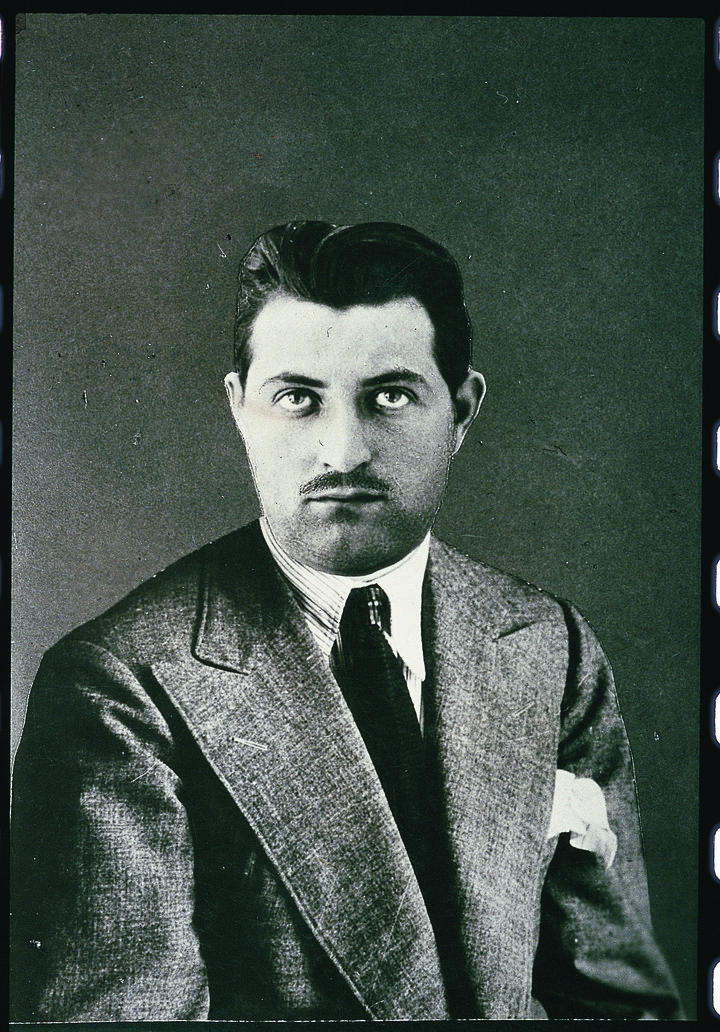
\includegraphics[width=0.5\textwidth]{../Images/SeverinoDiGiovanni.jpg}
 \caption{Severino Di Giovanni, el autor de este apunte. Un anarquista
   libertario, murió luchando por la libertad. Como él, otros miles han muerto
   para que nosotros gocemos de los derechos que tenemos. No te dejes engañar
   por los tristes pregoneros del egoísmo. Amá a tu prójimo y no olvides que si
   sus derechos se vulneran, los tuyos también. Ayudá a tu compañero de estudio,
 defendé tu universidad. }
 \end{figure}

\pagebreak

\tableofcontents
\newpage

\section{Read me}




\subsection{¿Por qué está en inglés?}

Estas notas fueron tomadas en un setup de NeoVim + LaTex a medida que los
apuntes originales de la materia eran estudiados. Los \textit{keybindings} de
NeoVim son incómodos si el teclado está en castellano. Las opciones eran $(a)$
castellano sin tildes o $(b)$ inglés. Pero $(a)$ es una aberración. $\therefore
$ $(b)$

\subsection{¿Qué hay en estas notas? ¿Debo confiar en ellas?}

These are my notes on computability theory. They may contain errors and are
should in no case substitute the text provided by professors. It has, however,
two advantages: it is very brief and to the point, and it contains solutions to
a lot of problems in each section.

\subsection{Definiciones preliminares}

The only definitions that ought to be known first-hand are the following.

Let $\Sigma$ denote an arbitrary language, $\omega := \mathbb{N} + \{
0\}$, and $n, m \geq 0$ fixed elements in $\omega$. Then: 

\begin{itemize}
    \item A $\Sigma$-mixed function is a function s.t. $\mathcal{D}_f \subseteq
        \omega^n \times \Sigma^{*m} \mapsto \varphi$ with either $\varphi =
        \omega$ or $\varphi = \Sigma^{*}$.
    \item A $\Sigma$-mixed function is $\Sigma$-effectively computable if we can
        find some algorithmic procedure that, given an input in $\omega^n \times
        \Sigma^{*m}$, outputs the value of $f(\overrightarrow{x},
        \overrightarrow{\alpha})$. 
    \item Any set $S \subseteq \omega^{n} \times \Sigma^{*m}$ is termed a
        $\Sigma$-mixed set. 
    \item If there is an algorithmic procedure that enumerates $S$, we say $S$
        is $\Sigma$-effectively enumerable. 

    \item If there is an algorithmic procedure that decides the belonging to
        $S$, we say $S$ is $\Sigma$-effectively computable.
\end{itemize}

Here, the notion of "algorithmic procedure" is non-rigorous. The principal
subject of this study are three formalizations of this concept: Turing
computability, recursive computability (Godel), and imperative
computability (von Neumann).

\pagebreak

\section{Coding infinite tuples}

We define $\omega^{\mathbb{N}} := \{ (s_1, s_2, \ldots) : s_i \in \omega \}$ and
$\omega^{\left[ \mathbb{N} \right] } \subseteq \omega^{\mathbb{N}} := \{(s_1,
s_2, \ldots) : s_i \in \omega \land \exists k \in \mathbb{N} : i \geq k
\Rightarrow s_i = 0\}$. 

\subsection{The $i$th prime function}

We define 

\begin{align*}
    pr : \mathbb{N} &\mapsto \omega  \\ 
    n &\mapsto \text{ the $n$th prime number}
\end{align*}

\begin{theorem}
    For all $x \in \mathbb{N}$ there is a unique infinituple $\overrightarrow{s}
    \in \omega^{[\mathbb{N}]}$ s.t. 

    \begin{align*}
        x = \prod_{i=1}^{\infty} pr(i)^{s_i}
    \end{align*}
\end{theorem}

The theorem follows trivially from the definition of $\omega^{[\mathbb{N}]}$ and
the fundamental theorem of arithmetic. 



\begin{theorem}
    If $p, p_1, \ldots, p_m$ are prime ($m \geq 1$) and $p \mid p_1 \ldots p_m$,
    then $p = p_i$ for some $i$.
\end{theorem}


\small
\begin{quote}

\textbf{Proof.} Assume $p \mid p_1 \ldots p_m$. $\therefore $ $p \leq p_1 \ldots
p_m$. The uniqueness of the prime factorization tells us that $p_1 \ldots p_n
$ are factors of a unique integer $x$.

Assume $p \not\mid p_j$ for any $j = 1, \ldots, m$. $\therefore $ $p$ is a prime
factor of $p_1 \ldots p_m$ distinct from $p_j$ for all $p_j$. $\therefore $ $x = p_1
\ldots p_m p \neq x$. $\therefore $  $\bot$

$\therefore $ $p \mid p_i$ for some $i = 1, \ldots, m$. $\blacksquare$

\end{quote}
\normalsize


We use $\left\langle  s_1, s_2, \ldots  \right\rangle$ to denote the number $x =
\prod_{n=1}^{\infty} pr(n)^{s_n}$. We use $(x)_i$ to denote $s_i$ in said tuple
and $(x)$ to denote the infinituple itself.

\begin{theorem}
    The functions 

    \begin{align*}
        \mathbb{N} &\mapsto \omega^{[\mathbb{N}]} &
        \omega^{[\mathbb{N}]}&\mapsto \mathbb{N} \\  
        x &\mapsto (x) = \left( (x)_1, (x)_2, \ldots \right) & (s_1, s_2,
        \ldots)&\mapsto \left\langle  s_1, s_2,\ldots  \right\rangle
    \end{align*}

    are bijections each the inverse of the other.
\end{theorem}

The theorem should be intuitive. The function that maps a number $x$ to the
infinituple of its prime exponents is the inverse of the function which takes an
infinituple and maps it to the product of its prime factors with the
corresponding exponents.

\begin{theorem}
    $$(x)_i = \max_{t} \left( pr(i)^{t} \mid x \right) $$
\end{theorem}


\small
\begin{quote}

    \textbf{Proof.} Let $x \in \mathbb{N}$ be s.t. $x = p_1^{s_1} \ldots
    p_m^{s_m}$ with $p_j$
prime and $m_j \neq 0$ for all $j = 1, \ldots, m$. Evidently $(x)_i = s_i$. 

Let $x \in \mathbb{N}$ and

\begin{align*}
    \mathscr{P}_i  := \left\{ t \in \omega : pr(i)^t \mid x \right\} 
\end{align*}

Since $\mathscr{P}_i \subseteq \mathbb{N}$ is necessary finite it has a maximum $
m_i$. The fundamental theorem of arithmetic directly gives $x = pr(1)^{m_1}
pr(2)^{m_2} \ldots$ Then by definition $m_i = (x)_i$. $\blacksquare$


\end{quote}
\normalsize


We define 

\begin{align*}
    Lt : \mathbb{N} &\mapsto \omega \\ 
    x &\mapsto \begin{cases}
        \max_{i} ~ (x)_i \neq 0 & x \neq 1 \\ 
        0 & x = 1
    \end{cases}
\end{align*}

The function returns the index of the maximum prime factor (that is not
zero-exponentiated) in the factorization of $x$. Since, in this factorizations,
all prime factors beyond $Lt(x)$ are zero, $Lt(x)$ can be understood as an
upper bound of the factorization. This is formalized in the following theorem.

\begin{theorem}
    \begin{align*}
        x = \prod_{i=1}^{Lt(x)}  pr(i)^{(x)_i}
    \end{align*}
\end{theorem}


\small
\begin{quote}


\begin{problem}
    Prove the previous theorem.
\end{problem}

$x = \prod_{i=1}^{\infty} pr(i)^{(x)_i} \land (x) \in
\omega^{[\mathbb{N}]}$ $\therefore$  $\exists k \in \omega :  i
\geq k \Rightarrow (x)_i =
0$ $\therefore $ $x = \prod_{i=1}^{k - 1} pr(i)^{(x)_i} \times \prod_{i=k}^{\infty}
pr(i)^{0} = \prod_{i=1}^{k-1} pr(i)^{(x)_i} $. But $k - 1 := \max_{i} \left(
(x)_i \neq 0 \right) := Lt(x)$. $\blacksquare$


\end{quote}
\normalsize

Prime numbers closely relate to set enumerability. The reason is that the prime
decomposition of a number associates to any unique $x \in \mathbb{N}$ an
infinite number of inters $(x)_1, (x)_2, \ldots$. Say we want to generate
all possible pairs $(x, y, z) \in \omega^3$ given a unique input $x \in
\mathbb{N}$. Then, letting $(x, y, z) = \left( (x)_1, (x)_2, (x)_3 \right) $, we
have 

\begin{align*}
    x = 1 &\mapsto (0, 0, 0)\\ 
    x = 2 &\mapsto (1, 0, 0)\\
    x = 3 &\mapsto (0, 1, 0)\\
    x = 4 &\mapsto (2, 0, 0)\\
    x = 5 &\mapsto (0, 0, 1)\\
    x = 6 &\mapsto (1, 1, 0)\\ 
    x = 7 &\mapsto (0, 0, 0)\\
    x = 8 &\mapsto (3, 0, 0)\\
    x = 9 &\mapsto (0, 2, 0)\\ 
      &\vdots
\end{align*}

It is easy to see that any $(x, y, z) \in \omega^3$ is reached. This generalizes
to $\omega^n, n \in \omega$ and to $\omega^{n} \times \Sigma^{*m} $ via the
$*^{\leq}$ function (which we shall study in the following section).

\subsection{Orders over $\Sigma$}

Let $\Sigma$ an alphabet with $n$ symbols. We want to find a bijection between $\omega$ and
$\Sigma^{*}$ assuming some order $\leq$ over $\Sigma$. Let $s^{\leq} :
\Sigma^{*} \mapsto \Sigma^{*}$ be


\begin{align*}
    s^{\leq} \left( (a_n)^m \right)  &= (a_1)^{m + 1} & m \geq 0\\ 
    s^{\leq} \left( \alpha a_i (a_n)^{m} \right) &= \alpha a_{i+1} (a_1)^{m} & 1
    \leq i < n, m \geq 0
\end{align*}

This function enumerates the language ordered $\Sigma$. For example, consider
$\Sigma = \{@, !\}$ with $@ < !$. Then 

\begin{align*}
    s^{\leq}( \varepsilon ) &= s^{\leq}( !^{0} ) = @\\
    s^{\leq}( @ ) &= s^{\leq}( \varepsilon @ (!)^{0} ) = \varepsilon ! \varepsilon = ~!
    \\ 
    \vdots
\end{align*}

Repeated application of this logic outputs the following enumeration: 

\begin{align*}
    @, !, @@, @!, !@, !!, @@@, @@!, @!@, @!!, !@@, !@!, !!@, !!!, \ldots
\end{align*}

The reason why $s^{\leq}( \beta  )$ enumerates the language is that every $\beta
$ is either of the form $(a_n)^{m}$ or $\alpha a_i (a_n)^{m}$. This is, it is
either a word with only the last character to a certain exponent, or a word with
some subchain before the last character to a certain exponent.

Now we are ready to define a bijection between $\omega$ and $\Sigma^{*}$. Let 

\begin{align*}
    *^{\leq} : \omega &\mapsto \Sigma^{*} \\ 
    x &\mapsto \begin{cases}
        \varepsilon & x = 0 \\ 
        s^{\leq} \left( *^{\leq} \left( i \right)  \right) & x = i + 1
    \end{cases}
\end{align*}

For example, using the same alphabet as before, this function maps 

\begin{align*}
    0 &\mapsto \varepsilon \\ 
    1 &\mapsto @ \\ 
    2 &\mapsto ! \\ 
    3 &\mapsto @@ \\ 
    4 &\mapsto @! \\ 
    5 &\mapsto !@ \\ 
    6 &\mapsto  !! \\ 
    7 &\mapsto  @@@ \\ 
      &\vdots
\end{align*}

Now, observe that any $\alpha \in \Sigma^{*}$ is a concatenation of unique
symbols, and that each of this unique symbols is the $i$th element of
$\Sigma^{*}$ for some $i$. We write to express this $\alpha = a_{i_k}\ldots
a_{i_0}$ where $i_{k}, i_{k-1}, \ldots, i_{k_0} \in \{ 1, \ldots, n\}$. Then we
define the inverse of the previous function as follows: 

\begin{align*}
    \#^{\leq} : \Sigma^{*} &\mapsto \omega \\ 
    \varepsilon & \mapsto 0 \\ 
    a_{i_k} \ldots a_{i_0} &\mapsto i_k n^{k} + \ldots + i_0 n^0
\end{align*}

For example, consider $\alpha = @!@ = a_{1} a_2 a_1$. Then $\#^{\leq}( \alpha )
= 1 \times 2^2 + 2 \times 2^1 + 1 \times 2^0 = 4 + 4 + 1 = 9$. It is easy to
verify that $*^{\leq}( 9 ) = @!@$.

Thus, the functions given produce a perfect bijection between numbers and words.
Each word can be univocally determined by its numeric position in the language;
each number can be univocally determined by a word whose position in the
language is that number. 

\begin{theorem}
    Let $n \geq 1$. Then any $x \in \mathbb{N}$ is uniquely written as $x = i_k
    n^k + i_{k-1} n^{k-1} + \ldots + i_0 n_^0$ with $k \geq 0, 1 \leq i_j \leq
    n$ for all $j$.
\end{theorem}

\subsection{Extending the order to words}

We can extend $\leq$ from $\Sigma$ onto $\Sigma^{*}$ by letting $\alpha \leq
\beta $ if and only if $\#^{\leq}(\alpha) \leq \#^{(\leq)}(\beta )$.

\pagebreak


\section{Enumerable and computable sets}

Let $\mathcal{F} : \mathcal{D}_{\mathcal{F}} \subseteq \omega^{k} \times \Sigma^{*l} \to \omega^n
\times \Sigma^{*m}$. We define $\mathcal{F}_{(i)} = p_i^{n, m} \circ
\mathcal{F}$. Then

\begin{align*}
    \mathcal{F}_{(i)} &: \mathcal{D}_{\mathcal{F}} \subseteq \omega^{k} \times
    \Sigma^{*l}  \mapsto \omega & 1 \leq i \leq n\\
    \mathcal{F}_{(i)} &: \mathcal{D}_{\mathcal{F}} \subseteq \omega^{k} \times
    \Sigma^{*l} \mapsto  \Sigma^{*} & n + 1 \leq i \leq m
\end{align*}

We say a set $S \subseteq \omega^n \times \Sigma^{*m} $ is $\Sigma$-effectively
enumerable  if it is empty or there is a function $\mathcal{F} : \omega \to
\omega^n \times \Sigma^{*m}$ s.t. $Im_{\mathcal{F}} = S$ and $\mathcal{F}_{(i)}$
is $\Sigma$-computable for all $1 \leq i \leq n + m$.

\begin{theorem}
    A non-empty set $S \subseteq \omega^n \times \Sigma^{*m}$ is
    $\Sigma$-effectively enumerable if and only if there is an effective
    procedure $\mathcal{P}$ s.t. 

    \begin{itemize}
        \item The input space is $\omega$
        \item $\mathcal{P}$ halts for all $x \in \omega$ 
        \item The output set is $S$---i.e. whenever $\mathcal{P}$ halts, it
            outputs an element of $S$, and for every $(\overrightarrow{x},
            \overrightarrow{\alpha}) \in S$ there is some input $x \in \omega$
        s.t. $\mathcal{P}(x) \mapsto_{\text{halting}} (\overrightarrow{x},
        \overrightarrow{\alpha})$.
    \end{itemize}
\end{theorem}


\small
\begin{quote}

\begin{problem}
    Let $F : \left\{ (x, \alpha) \in  \omega \times \Sigma^{*} : |\alpha|^x
        \equiv 0 \mod 2
    \right\} \mapsto \omega^2 \times \Sigma^{*}$ be defined as follows: 

    \begin{align*}
        F(x, \alpha) = (x, x^2 + |\alpha|, \varepsilon)
    \end{align*}

    Provide $F_{(1)}, F_{(2)}, F_{(3)}$. What function is $[F_{(1)}, F_{(2)},
    F_{(3)}]$?
\end{problem}

By definition, $F_{(i)} = p_i^{1, 1} \circ F$. Then 

\begin{align*}
    F_{(1)}(x, \alpha) &= x \\
    F_{(2)}(x, \alpha) &= x + |\alpha| \\
    F_{(3)}(x, \alpha) &= \varepsilon
\end{align*}

It is evident that the composition given results in $F$.

\begin{problem}
    Prove that $F = \left[ F_{(1)}, \ldots, F_{(n + m)} \right] $.
\end{problem}

Let $G := \left[ F_{(1)}, \ldots, F_{(n+m)} \right] $. 

$\therefore $  $G(\vec{x}, \vec{\alpha}) = \left( p_1^{n, m} \circ F(\vec{x},
\vec{\alpha}), \ldots, p_{n+m} \circ F(\vec{x}, \vec{\alpha})   \right)  =
F(\vec{x}, \vec{\alpha}) $ $\blacksquare$



\end{quote}
\normalsize

\begin{theorem}
    Let $S \subseteq \omega^{n} \times \Sigma^{*m} $. The following statements are equivalent. 

    \textit{(1)} $S$ is $\Sigma$-effectively enumerable. 

    \textit{(2)} $S$ is the domain of a $\Sigma$-effectively computable function
    $f$.  

    \textit{(3)} $S$ is the image of a function $F: \mathcal{D}_f \subseteq
    \omega^{n} \times \Sigma^{*m} \mapsto S$ s.t. each $F_{(i)}$ is
    $\Sigma$-effectively computable.
\end{theorem}

That $(1) \Leftrightarrow (3)$ is trivial. $(1) \Leftrightarrow (2)$ can be proven as
follows. 


\small
\begin{quote}

\textbf{Proof.} $(\Rightarrow)$. Assume $S$ is $\Sigma$-effectively enumerable.
Then there is a procedure $\mathbb{P}$ s.t. for any $x \in  \omega$ the
procedure outputs a value of $S$, and all values of $S$ are mapped. Consider the
procedure $\mathbb{P}'$ s.t. given an input $(\vec{x}, \vec{\alpha}) \in S$ it
\textit{a.} computes $\mathbb{P}$ with input  $x = 0, 1, \ldots$ until
$\mathbb{P}$ maps to $(\vec{x}, \vec{\alpha})$ and \textit{b.} then returns $x$.
Evidently $\mathbb{P}'$ computes the inverse of the function computed by
$\mathbb{P}$. Observe that $\mathbb{P}'$ will only halt if $(\vec{x},
\vec{\alpha}) \in S$. Then $S$ is the domain of a $\Sigma$-effectively
computable function.

$(\Leftarrow)$ Assume $S$ is the domain of a $\Sigma$-effectively computable
function. Let $(\vec{w}, \vec{\beta})$ an arbitrary element of $S$. Consider a
procedure $\mathbb{P}$ which does the following with an input $x \in \omega$.

\begin{quote}
    \textit{(1)} Produce the enumeration of $\omega \times \omega^{n} \times
    \Sigma^{*m} $ given by $x$. This will produce a variable $(t, \vec{x},
    \vec{\alpha})$.

    \textit{(2)} Run $t$ steps of $\mathbb{P}_f$ with input $(\vec{x},
    \vec{\alpha}) $. If the program terminated, return $(\vec{x},
    \vec{\alpha})$. If not, return $(\vec{w}, \vec{\beta})$.
\end{quote}

Evidently, $\mathbb{P}$ enumerates $S$. $\blacksquare$

\end{quote}
\normalsize

Since any $\Sigma$-effectively computable set is $\Sigma$-effectively
enumerable, point \textit{(1)} of the previous theorem can be substituted by $S$
is $\Sigma$-effectively enumerable---with some loss of generality.

\begin{theorem}
    Let $f : \mathcal{D}_f \subseteq \omega^{n} \times \Sigma^{*m} \mapsto \varphi$ with
    $\varphi$ either $\omega$ or $\Sigma^{*}$. Let $S \subseteq \mathcal{I}_f$.
    Then if $f$ is $\Sigma$-effectively computable and $S$ is
    $\Sigma$-effectively enumerable, $f^{-1}(S) = \left\{ (\vec{x},
    \vec{\alpha}) : f(\vec{x}, \vec{\alpha}) \in S \right\} $ is
    $\Sigma$-effectively enumerable .
\end{theorem}



\small
\begin{quote}

\textbf{Proof.} Assume $f$ is $\Sigma$-effectively computable and $S \subseteq
\mathcal{I}_f$ is $\Sigma$-effectively enumerable. Let $(\vec{w}, \vec{\beta}) $
an arbitrary element of $f^{-1}(S)$. Consider the following
effective procedure operating over an input $x \in \omega$: 

\begin{quote}

    \textit{(0)} If $x = 0$ return $(\vec{w}, \vec{\beta})$. Else proceed.

    \textit{(1)} Enumerate an element of $s \in S$ using input $x$. 

    \textit{(2)} Use $(\vec{x}, \vec{\alpha}) := ( (x)_1, \ldots, (x)_n, *^{\leq}( (x)_{n+1}), \ldots,
    *^{\leq}( (x)_m ))$ to compute a value of $f(\vec{x}, \vec{\alpha})$. 

    \textit{(3)} If $f(\vec{x}, \vec{\alpha}) = s$ return $(\vec{x},
    \vec{\alpha}) $. Else return $(\vec{w}, \vec{\beta}) $.
\end{quote}

Evidently, the procedure enumerates $f^{-1}(S)$. $\blacksquare$

\end{quote}
\normalsize


The theorem states that the set of inputs which map to a region of a computable
function's range is enumerable if that region is enumerable.

\begin{theorem}
    If $f : \mathcal{D}_f \subseteq \omega^{n} \times \Sigma^{*m} \mapsto
    \varphi$ with $\varphi$ either $\omega$ or $\Sigma^{*}$, then if $S
    \subseteq \mathcal{D}_f$ is $\Sigma$-effectively enumerable, $f_{| S}$ is
    $\Sigma$-effectively computable.
\end{theorem}



\subsection{Prime numbers and enumerable sets}

Let $\Sigma \neq \emptyset$ be an alphabet with a total order $\leq$. Let $S
\subseteq \omega^{n} \times \Sigma^{*m}$ a $\Sigma$-mixed set of arbitrary
dimensions. Notice that for any $n$-tuple $(x_1, \ldots, x_n)$, with $x_i \in
\omega$, we can find a corresponding $\varphi \in \mathbb{N}$ s.t. 

$$
\varphi = 2^{x_1}3^{x_2} \ldots pr(n)^{x_n}
$$

In other words, $(x_1, \ldots, x_n)$ corresponds to the exponents of the $n$
prime factors of a unique natural number. At the same time, the $m$-tuple
$(\alpha_1, \ldots, \alpha_m)$ corresponds to a unique $\psi \in \mathbb{N}$
s.t. 

$$
\psi = 2^{y_1}3^{y_2}\ldots pr(m)^{y_m}
$$

where $\alpha_j = *^{\leq}(y_j)$. In other words, $(\alpha_1, \ldots, \alpha_m)$
corresponds to a unique natural number whose $m$ prime factors have exponents
given by the position of each word in the language.

Both of these relations come from the uniqueness of prime factorizations.
They provide a way to enumerate $\Sigma$-mixed sets. In
particular, if $S$ is $\Sigma$-total we enumerate it mapping each $x \in \omega$
to $\big((x)_1, \ldots, (x)_n, *^{\leq}((x)_{n+1}), \ldots, *^{\leq}((x)_m)\big)$. If
$S$ is not $\Sigma$-total, then one can still enumerate it assuming that it is
$\Sigma$-computable. Indeed, one maps $x$ to the corresponding $(n+m)$-tuple
described above if the tuple is in $S$, and leaves the procedure undefined (or
without halt) otherwise. This can be expressed as follows:

Because $\Sigma$-total sets are enumerable (as pointed out above), any
$\Sigma$-mixed set that is $\Sigma$-computable is enumerable (via restriction
of the $\Sigma$-total enumeration).

\begin{theorem}
    If $S \subseteq \omega^{n} \times \Sigma^{*m} $ is $\Sigma$-effectively
    computable, then it is $\Sigma$-effectively enumerable.
\end{theorem}

\small
\begin{quote}



\begin{problem}
    Prove the following statement: If $S \subseteq \omega$ and $f : S \mapsto
    \omega$ is $\Sigma$-effectively computable, then 
    
    \begin{align*}
        A = \left\{ x \in  S : x \text{ is even } \land x / 2 \in S \land f(x) = f(x
        / 2) \right\} 
    \end{align*}

    is $\Sigma$-effectively enumerable.
\end{problem}

Assume $f$ is $\Sigma$-effectively computable.  $\therefore S$ is
$\Sigma$-effectively enumerable. 

Let $\mathbb{P}_S$ be the procedure that enumerates $S$. Let $\mathbb{P}_f$
denote the procedure which computes $f$, $w \in S$ fixed and arbitrary, and $\mathbb{P}$ with input $x \in
\omega$ the following
procedure: 

\begin{quote}

    \textit{(0)} If $x = 0$ return $w$ and finish. 

    \textit{(1)} Use $\mathbb{P}_S$ twice, with inputs $(x)_1, (x)_2$
    respectively, to produce elements $s_1, s_2 \in S$. 

    \textit{(2)} Check if $s_1$ is even (this is trivially effectively
    computable). If it isn't, return $w$ and finish. 

    \textit{(3)} Check if $s_2 = s_1 / 2 $. If it isn't, return $w$ and finish.

    \textit{(4)} Use $\mathbb{P}_f$ to compute $f(s_1), f(s_2)$ and compare
    these values. If they are not equal, return $w$ and finish. 

    \textit{(5)} Return $s_1$.
\end{quote}

Evidently, $\mathbb{P}$ enumerates $A$.


\end{quote}
\normalsize



\pagebreak
\section{Turing}

From now on, we will attempt formalizations of three so far informal concepts: 

\begin{itemize}
    \item $\Sigma$-effectively computable functions
    \item $\Sigma$-effectively computable sets
    \item $\Sigma$-effectively enumerable sets
\end{itemize}

The first formalization is given by Turing.

\subsection{Turing machine}

A Turing machine is a $7$-uple $M = \left( Q, \Sigma, \Gamma, \delta, q_0, B, F
\right) $ where

\begin{itemize}
    \item $Q$ is a set of states 
    \item $\Gamma \supset \Sigma$ is an alphabet
    \item $\Sigma$ is the input alphabet
    \item $B \in \Gamma - \Sigma$ is a blank symbol 
    \item $\delta : \mathcal{D}_\delta\subseteq Q \times \Gamma \mapsto Q \times \Gamma \times \left\{
        L, R, K\right\}   $ 
    \item $q_0 \in Q$ is the initial state 
    \item $F \subseteq Q$ is the set of final states
\end{itemize}


\small
\begin{quote}

\begin{problem}
    If $M$ a Turing machine then $\delta$ is a $\Sigma$-mixed function.
\end{problem}

A function is said to be a $\Sigma$-mixed function if $\mathcal{D}_f \subseteq
\omega^n \times \Sigma^{*m}$ for some $n, m \geq 0$ and $\mathcal{I}_f \subseteq
\omega$ or $\mathcal{I}_f \subseteq \Sigma^{*}$. The $\delta$ function satisfies
neither of these properties; its domain is a set of states $Q \times \Gamma \not\subseteq
\Sigma^{*m}$ and its image is a set of sets.

\begin{problem}
    If $M$ a Turing machine, $\mathcal{D}_{\delta}$ is a $\Sigma$-mixed set.
\end{problem}

A set $S$ is said to be $\Sigma$-mixed iff $S \subseteq \omega^n \times
\Sigma^{*m}$ for some $n, m \geq 0$. We have already mentioned that
$\mathcal{D}_\delta = Q \times \Gamma \not\subseteq \omega^n \times \Sigma^{*m}$ for any $n,
m$. Then $\mathcal{D}_\delta$ is not $\Sigma$-mixed.

\begin{problem}
    If $M$ a Turing machine, then $\mathcal{I}_{\delta}$ is $\Sigma$-mixed.
\end{problem}

False again.

\end{quote}
\normalsize


\subsection{Deterministic Turing machine}

A Turing machine is said to be deterministic iff $|\delta(p, \sigma)| \leq 1$
for all $p \in Q, \sigma \in \Gamma$. 

\subsection{Instantaneous descriptions}

An instantaneous description is a word of the form $\alpha q \beta $ where
$\alpha, \beta \in \Gamma^{*}, [\beta]_{|\beta |} \neq B$ and $q \in Q$. If the
instantaneous description is $\alpha_1 \alpha_2 \ldots \alpha_n q \beta_1
\beta_2 \ldots \beta_m B B B \ldots$, we read: \textit{The Turing
machine is in state $q$ and it is reading $\beta_1$}. We use $\mathbb{D}$ to
denote the set of instantaneous descriptions. We define 

\begin{align*}
    St : \mathbb{D} &\mapsto  Q \\ 
    d &\mapsto \text{Only symbol of $Q$ that is in $d$}
\end{align*}


\small
\begin{quote}

\begin{problem}
    Let $d \in \mathbb{D}$ an instantaneous description. Then $Ti(d)$ is a
    triple.
\end{problem}

False: $d$ is not a triple but a single element of $(\Gamma \cup Q)^{*}$.

\begin{problem}
    If $d \in \mathbb{D}$ then $St(d) = d \cap Q$
\end{problem}

False. The operation $d \cap Q$ makes no sense, insofar as $d$ is a symbol. It
would be correct to say $St(d) = \{d_1, d_2, \ldots, d_m\} \cap Q$ where $d_i$ are
the characters in the word $d$.


\end{quote}
\normalsize

\subsection{State transitions}

\small
\begin{quote}

Given $\alpha \in (\Gamma \cup Q)^*$ we define 

\begin{align*}
    \left\lfloor \varepsilon \right\rfloor  &= \varepsilon \\ 
    \left\lfloor \alpha \sigma  \right\rfloor  &= \alpha \sigma \text{   if } \sigma \neq B \\ 
    \left\lfloor \alpha B \right\rfloor &= \left\lfloor  \alpha \right\rfloor
\end{align*}

Thus, $\left\lfloor \alpha \right\rfloor$ removes the trailing blank symbols of $\alpha$ (if any).
\end{quote}
\normalsize 

Given $d_1, d_2 \in \mathbb{D}$ with $d_1 = \alpha p \beta $, we say $d_1 \vdash
d_2$ if, given $\alpha \in \Gamma, \alpha, \beta \in  \Gamma^*, p, q \in Q$, one
of the following three cases hold.

~

\textit{(Case 1)} $\alpha \neq \varepsilon$, and

\begin{align*}
    \delta \left( p, \left[ \beta B \right]_1  \right) \ni (q, \sigma, L)
\end{align*}

and 
$$d_2 = \left\lfloor \alpha {}^{\curvearrowleft} q [\alpha]_{|\alpha|} \sigma
{}^{\curvearrowright} \beta  \right\rfloor$$

\small 
\begin{quote}
    \textit{Interpretation.} The Turing machine at state $p$ will write $\sigma$
    at its current position, transition to state $q$, and move to the left. 

    \textit{Example.} Let $\Sigma = \{ @, \#\}$. Assuming $\delta (p) = \{ (q,
    \#, L) \}$, then the following is an example of
    \textit{Case 1}.
    
    \begin{align*}
        &@ ~ \# ~ @ ~ p ~ @ ~ @ ~ @ ~ B ~ B ~ B \vdash  @ ~ \# ~q ~ @ ~ \# ~ @ ~ @ ~ B ~ B
        ~ \ldots
    \end{align*}
\end{quote}
\normalsize 

~ 

\textit{(Case 2)} 

\begin{align*}
    \delta \left( p, \left[ \beta B \right]_1  \right) \ni (q, \sigma, R)
\end{align*}

and 

$$d_2 = \alpha \sigma q {}^{\curvearrowright} \beta $$

\small 
\begin{quote}
    \textit{Interpretation.} The Turing machine at state $p$ will write $\sigma$
    at its current position, transition to state $q$, and move to the left. 

    \textit{Example.} Let $\Sigma = \{ @, \#\}$. Assuming $\delta (p) = \{ (q,
    \#, R) \}$, then the following is an example of
    \textit{Case 2}.
    
    \begin{align*}
        &@ ~ \# ~ @ ~ p ~ @ ~ @ ~ @ ~ B ~ B ~ B \vdash  @ ~ \# ~@ ~ \# ~ q ~ @ ~
        @~ B ~ B
        ~ \ldots
    \end{align*}
\end{quote}
\normalsize 


\textit{(Case 3)} 

\begin{align*}
    \delta \left( p, \left[ \beta B \right]_1  \right) \ni (q, \sigma, K)
\end{align*}

and 

$$d_2 = \left\lfloor \alpha q \sigma {}^{\curvearrowright} \beta  \right\rfloor $$

\small 
\begin{quote}
    \textit{Interpretation.} The Turing machine at state $p$ will write $\sigma$
    at its current position, transition to state $q$, and stay at the same
    position.

    \textit{Example.} Let $\Sigma = \{ @, \#\}$. Assuming $\delta (p) = \{ (q,
    \#, K) \}$, then the following is an example of
    \textit{Case 2}.
    
    \begin{align*}
        &@ ~ \# ~ @ ~ p ~ @ ~ @ ~ @ ~ B ~ B ~ B \vdash  @ ~ \# ~@ ~ q ~ \# ~  @ ~
        @~ B ~ B
        ~ \ldots
    \end{align*}
\end{quote}
\normalsize 

We say $d \vdash^n d'$ if there are $d_1, \ldots, d_{n+1}$ s.t. $d = d_1, d' =
d_{n+1}$, and $d_i \vdash d_{i + 1}$ for all $i = 1, \ldots, n$. Observe that $d
\vdash^0 d'$ if $d = d'$. Finally, we denote $d \vdash^{*} d'$ iff $(\exists n
\in \omega) ~ d \vdash^n d'$.


\small
\begin{quote}

\begin{problem}
    Determine true or false for the following propositions.
\end{problem}

\textit{(1) $d \vdash d$ for all $d \in \mathbb{D}$}. The proposition is false.
It is trivial to find a counterexample.

\textit{(2) If $\alpha p \beta  \not\vdash  d$ for every $d \in \mathbb{D}$,
then $\delta(p, [\beta B]_1) = \emptyset$}. Assume $\alpha p \beta \not\vdash d$
for every $d \in \mathbb{D}$. Assume $\delta(p, [\beta B]_1) \neq \emptyset$.
Then there must be some $\{(q, \sigma, D)\}$ with $D \in \left\{ L, R, K
\right\} $ that corresponds to this evaluation of $\delta$. But then there would
exist some $d$, given by the case division above and depending on the value of
$D$, s.t. $\alpha p \beta \vdash d$. But this is a contradiction. The statement
is true.

\textit{(3) If $(p, \alpha, L) \in \delta(p, a)$ then $pa \not\vdash d$ for all
$d \in \mathbb{D}$}. This is correct. Remember that for a transition to the left
to be defined we require that a substring $\alpha \neq \varepsilon$ precede the
Machine's head. (See \textit{Case 1}, requirement $\alpha \neq \varepsilon$.) But
here $d_1 = pa$ has an initial segment $\varepsilon$ preceding $p$. Then $pa \neq
d$ for any $d$. The statement is true.

\textit{(4)} \textit{  Given $d_1, d_2 \in \mathbb{D}$, if $d_1 \vdash d_2$ then
$|d_1| \leq |d_2| + 1$. } It makes no sense to say $|d_1| \leq |d_2| + 1$
insofar as an instantaneous description contains infinitely many symbols $B$ at
the end. So the statement, as it is phrased, is false. However, consider the
alternative postulate: $d_1 \vdash d_2 \Rightarrow |\left\lfloor d_1
\right\rfloor| \leq | \left\lfloor d_2 \right\rfloor | + 1$. Two instantaneous
description over the same machine always have the same number of symbols. So $ |
\left\lfloor d_1 \right\rfloor| = | \left\lfloor d_2 \right\rfloor | $, which
makes the statement trivially true.

\begin{problem}
    Prove that $M$ is deterministic iff for each $d \in \mathbb{D}$ there is
    \textit{at most} one $d' \in \mathbb{D}$ s.t. $d \vdash d'$.
\end{problem}

( $\Rightarrow$ ) Assume $M$ is deterministic. Then for any $d \in \mathbb{D}$
of the form $\alpha q \beta B B \ldots$, we have either $\delta(q) = \left\{
(q', \sigma, D) \right\} $ or $\delta(q) = \emptyset$. If $\delta(q) =
\emptyset$, then (by definition of $\vdash$) there is no instantaneous description $d'$ s.t. $d \vdash d'$.
If $\delta(q) = \left\{ (q', \sigma, D) \right\} $, then two cases are possible.
\textit{(1)} $d$ holds the assumptions sustaining the case definition of
$\vdash$, in which case the transition is uniquely determined by $(q',
\sigma, D)$. \textit{(2)} $d$ does not hold the assumptions sustaining the
case definition of $\vdash$ (e.g. $D = L, \alpha = \varepsilon$), in which case
there is by definition no $d'$ s.t. $d \vdash d'$

($\Leftarrow$) This does not hold!! Assume that, for all $d \in \mathbb{D}$,
there is at most one $d'$ s.t. $d \vdash d'$. 
 Consider the case where there is no $d'$ s.t. $d \vdash d'$. In the case where
 $\alpha = \varepsilon$ and

$$
\delta(q) = \{ (q', \sigma, L), (q'', \sigma', L) \}
$$

the machine is non-deterministic without violating the assumption. In other
words, that $d \vdash d'$ for at most one $d'$ does not imply that the machine
is deterministic.

\end{quote}
\normalsize


\subsection{Halting and languages}

Given $d \in \mathbb{D}$, we say $M$ halts starting from $d$ if there is some
$d' \in \mathbb{D}$ s.t. 

\begin{align*}
    &d \vdash^* d' \\ 
    &d' \not\vdash d'' \text{ for all } d'' \in \mathbb{D}
\end{align*}

We say a word $w \in \Sigma^{*}$ is accepted by a Turing machine $M$ \textit{by reach of final
state} if

\begin{align*}
    \exists d \in \mathbb{D} : \left\lfloor q_0 B w \right\rfloor \vdash^* d \land ~ St(d) \in F
\end{align*}

Observe that we do not require that $d \in St(d)$ satisfies $d \not\vdash d'$
for all $d' \in \mathbb{D}$. In other words, a machine may accept a word by
reach of final state and not halt.

The language accepted by a Turing machine is 

\begin{align*}
    \mathcal{L}(M) = \left\{w \in \Sigma^{*}:  w \text{ is accepted by reach of final state } \right\} 
\end{align*}

\small
\begin{quote}

\begin{problem}
    Let $\Sigma = \left\{ a, b \right\} $. Find a Turing machine $M$ that
    accepts the language $ \left\{ w \in \Sigma^{*} : |\omega|_a = 2|\omega|_b
    \right\} $
\end{problem}

As examples, here are some words accepted by the language: $\varepsilon, aab, baa,
ababaa, \ldots$ Our machine will operate in the following manner.

\textit{(1)} It will parse the string looking for a $b$; if a $b$ is found, it
replaces it with $y$, sets the head of the machine to the beginning, and
proceeds to parse for two $a$s and replace them with $x$s. This gives 

\begin{align*}
    \delta(q_0, \sigma) &= \begin{cases}
        \left\{ \left( q_1, y, L \right)  \right\} & \sigma = b\\
        \left\{ \left( q_0, \sigma, R \right)  \right\} & \sigma = a\\
        \left\{ \left( q_9, \sigma, L \right)  \right\} & \sigma = B
    \end{cases} \\
    \delta(q_1, \sigma) &= \begin{cases}
        \left\{ \left( q_1, \sigma, L \right)  \right\} & \sigma \neq \varepsilon
        \\ 
        \{ (q_2, \varepsilon, R) \} & \sigma = \varepsilon
    \end{cases}
\end{align*}

where $q_1$ resets the machine's head to the initial position. Now 

\begin{align*}
    \delta(q_2, \sigma) &= \begin{cases}
        \left\{ (q_3, x, R) \right\}  & \sigma = a \\ 
        \left\{ (q_2, \sigma, R) \right\}  & \sigma \neq a \\ 
    \end{cases}\\
    \delta(q_3, \sigma) &= \begin{cases}
        \left\{ (q_4, x, R) \right\}  & \sigma = a \\ 
        \left\{ (q_3, \sigma, R) \right\}  & \sigma \neq a \\ 
    \end{cases}
\end{align*}

The state $q_4$ occurs after two $a$s have been found to correspond to a single
$b$. Thus, we must return to $q_0$ with the machine head reset to its initial
position. 

\begin{align*}
    \delta(q_4, \sigma) = \begin{cases}
        \left\{ \left( q_4, \sigma, L \right)  \right\} & \sigma \neq \varepsilon
        \\
        \left\{ \left( q_0, \sigma, R \right)  \right\} & \sigma = \varepsilon 
    \end{cases}
\end{align*}

The only undefined state is $q_9$. This is the state reached after, in state
$q_0$, the string is parsed but no $b$ is found. If there is some $a$ left in
the string, then the word must not be accepted; but if no $a$ exists, the word
must be accepted. Thus, $q_9$ can parse from right to left looking for $a$s; if
$\varepsilon$ is reached without $a$s on the way, it should map to a final state.
If some $a$ is found, it should never halt.

\begin{align*}
    \delta(q_9, \sigma) = \begin{cases}
        \left[ \left( q_9, \sigma, L \right)   \right] & \sigma \neq\in \{a,
        \varepsilon\} \\
        \left[ \left( q_9, \sigma, K \right)   \right] & \sigma = a \\ 
        \left[ \left( q_\mathcal{F}, \sigma, K \right)   \right] & \sigma = \varepsilon \\ 
    \end{cases}
\end{align*}

where $q_{\mathcal{F}} \in F$ is the only final state. Of course, $\Gamma = \{a,
b, x, y, B\}, Q = \{ q_0, q_1, q_2, q_3, q_4, q_9, q_{\mathcal{F}}\}$.

\end{quote}
\normalsize

We say a word $w \in \Sigma^{*}$ is accepted by detention (or by a halt) if $M$
halts when starting from $ \left\lfloor q_0 B \omegam \right\rfloor  $. We
denote 

\begin{align*}
    \mathcal{H}(M) = \left\{ w \in \Sigma^{*}: w \text{ is accepted
    by detention} \right\} 
\end{align*}

\begin{theorem}
    Let $L \subseteq \Sigma^{*}$. Then the following statements are equivalent: 

    \textit{(1)} There is a Turing machine $M$ s.t. $L = L(M)$. 

    \textit{(2)} There is a Turing machine $M$ s.t. $L = \mathcal{H}(M)$.
\end{theorem}

\subsection{$\Sigma$-Turing computable functions}

To represent numbers on the Turing tape, we use the $i$ letter. Thus, we extend
the definition of a Turing machine ensuring that $i \in  \Gamma - \left( \{B\}
\cup \Sigma \right) $ is a symbol.

Let $f : \mathcal{D}_f \subseteq \omega^{n} \times \Sigma^{*m} \mapsto
\Sigma^{*}$ a $\Sigma$-mixed function. We say $f$ is $\Sigma$-Turing computable
if there is a deterministic Turing machine $M$ s.t. 

\begin{itemize}
    \item If $(\vec{x}, \vec{\alpha}) \in \mathcal{D}_f$, then there is a state
        $p \in Q$ s.t. 
        \begin{align*}
            \left\lfloor q_0 ~ B ~ i^{x_1} ~ B ~ \ldots ~ i^{x_n} ~ B ~ \alpha_1
            ~ B ~ \ldots ~ B ~ \alpha_m\right\rfloor \vdash^* \left\lfloor pB
            f(\vec{x}, \vec{\alpha}) \right\rfloor
        \end{align*} 

        and $\left\lfloor pBf(\vec{x}, \vec{\alpha}) \not\vdash d \right\rfloor$
        for all $d \in \mathbb{D}$.

    \item If $(\vec{x}, \vec{\alpha}) \in \omega^{n} \times \Sigma^{*m} -
        \mathcal{D}_f$, then the machine does not halt starting from  
        \begin{align*}
            \left\lfloor q_0 ~ B ~ i^{x_1} ~ B ~ \ldots ~ i^{x_n} ~ B ~ \alpha_1
            ~ B ~ \ldots ~ B ~ \alpha_m\right\rfloor 
        \end{align*}
\end{itemize}

When $f \mapsto \omega$, we analogously say a Turing machine computes $f$ iff

\begin{itemize}
    \item If $(\vec{x}, \vec{\alpha}) \in \mathcal{D}_f$, then there is a state
        $p \in Q$ s.t. 
        \begin{align*}
            \left\lfloor q_0 ~ B ~ i^{x_1} ~ B ~ \ldots ~ i^{x_n} ~ B ~ \alpha_1
            ~ B ~ \ldots ~ B ~ \alpha_m\right\rfloor \vdash^* \left\lfloor pB
            i^{f(\vec{x}, \vec{\alpha})} \right\rfloor
        \end{align*} 
        
        and $\left\lfloor pBi^{f(\vec{x}, \vec{\alpha})} \not\vdash d \right\rfloor$
        for all $d \in \mathbb{D}$.

    \item If $(\vec{x}, \vec{\alpha}) \in \omega^{n} \times \Sigma^{*m} -
        \mathcal{D}_f$, then the machine does not halt starting from  
        \begin{align*}
            \left\lfloor q_0 ~ B ~ i^{x_1} ~ B ~ \ldots ~ i^{x_n} ~ B ~ \alpha_1
            ~ B ~ \ldots ~ B ~ \alpha_m\right\rfloor 
        \end{align*}
\end{itemize}

If $M$ and $f$ satisfy the properties above, we say $f$ is computed by $M$.

\begin{theorem}
    If $f : \mathcal{D}_f \subseteq \omega^{n} \times \Sigma^{*m} \mapsto I \in
    \{\omega, \Sigma^{*}\}$ is computed by a Turing machine $M$, then $f$ is $\Sigma$-effectively
    computable.
\end{theorem}


\small
\begin{quote}

\begin{problem}
    Determine if the following statements are true or false.
\end{problem}

\textit{(1) If $M$ a deterministic turing machine and $M$ computes $f$, then
$\mathcal{L}(M) = \mathcal{D}_f$}. 

Since $M$ computes $f$, $M$ halts for any
$(\vec{x}, \vec{\alpha}) \in \mathcal{D}_f$ and does not halt for any $(\vec{x},
\vec{\alpha}) \not\in \mathcal{D}_f$. Then, by definition, $\mathcal{H}(M) =
\mathcal{D}_f$. This does not imply $\mathcal{L}(M) = \mathcal{D}_f$. However,
it does imply that there necessarily exists a Turing machine $M'$ s.t.
$\mathcal{L}(M') = \mathcal{D}_f$.

\textit{(2)}  \textit{ If $f, g$ are two functions and $M$ is a Turing machine that
computes $f$ and $g$, then $f = g$.} Assume the premise holds. Then
$\mathcal{H}(M) = \mathcal{D}_f = \mathcal{D}_g := \mathcal{D}$. Furthermore, for any
$(\vec{x}, \vec{\alpha}) \in \mathcal{D}$, the Turing machine halts with an
instantaneous description representing $f (\vec{x}, \vec{\alpha}) $. But since
it computes $g$, the instantaneous description also represents $g (\vec{x},
\vec{\alpha}) $. This implies $f (\vec{x}, \vec{\alpha}) = g (\vec{x},
\vec{\alpha}) $. Then $f = g$. The statement is true.

\textit{(3) Let $M$ a Turing machine and assume $M$ computes $f$ with $f$ a
$\Sigma$-total function. Then $M$ halts from $d$ for whichever $d \in
\mathbb{D}$}. It is true that, since $f$ is $\Sigma$-total, for any $(\vec{x},
\vec{\alpha}) \in \omega^{n} \times \Sigma^{*m} $, $f (\vec{x}, \vec{\alpha}) $
is defined. This does imply that every $d$ of the form $\left\lfloor q_0 i^{x_1}\ldots i^{x_n} \alpha_1
\ldots \alpha_m \right\rfloor$ is accepted (I skipped the possibly infinite $B$
symbols in the description). However, there is no restriction in $\mathbb{D}$ as
to the number of unit or alphabetic symbols which an arbitrary $d \in
\mathbb{D}$ may contain. Thus,  

\begin{align*}
    \mathbb{D}' \subseteq \mathbb{D} = \left\{ d \in \mathbb{D} : \left\lfloor d
    \right\rfloor = \left\lfloor q_0 i^{x_1} \ldots i^{x_k} \alpha_1 \ldots
\alpha_l \right\rfloor : k \neq n \lor l \not\in m  \right\} 
\end{align*}

satisfies $D' \not\subseteq \mathcal{H}(M)$.


\end{quote}
\normalsize




\pagebreak
\section{Godel}

\begin{definition}
    A set $S_1\times  \ldots  \times  S_n \times L_1 \times  \ldots \times  L_m$ is
    rectangular if $S_i \subseteq \omega, L_i \subseteq \Sigma^{*}$ for all $i$.
\end{definition}

\begin{lemma}
    $S$ is rectangular if and only if $(\overrightarrow{x},
    \overrightarrow{\alpha}) \in S \land (\overrightarrow{y},
    \overrightarrow{\beta}) \in S$ implies $(\overrightarrow{x},
    \overrightarrow{\beta}) \in S$.
\end{lemma}

\textit{Example}. The set $\{(0, \#\#), (1, \%\%\%)\}$ is not rectangular ($(1,
\#\#), (0, \%\%\%)$ are not in $S$.) Observe how this set cannot be expressed as
a product of subsets of $\omega$ and $\Sigma$. Thus, the concept of
\textit{rectangular set} is equivalent to \textit{a set formed via Cartesian
product}.

~

\textit{Notation.} If $f : \omega_1 \times \ldots \times \omega_n \times
\alpha_1 \times \alpha_m \to \Lambda$ we write $f \sim (n, m, \Lambda)$, and
read $f$ is of type $n, m$ to $\Lambda$.

\textit{Notation.} If $f_1, \ldots, f_n$ $\Sigma$-mixed functions, then 

\begin{align*}
    \left[ f_1, \ldots, f_2 \right](\overrightarrow{x}, \overrightarrow{\alpha})
    = \left( f_1(\overrightarrow{x}, \overrightarrow{\alpha}), \ldots,
    f_n(\overrightarrow{x}, \overrightarrow{\alpha}) \right) 
\end{align*}


\subsection{Primitive recursion} 

Let $R$ a $\Sigma$-mixed function s.t. $R \sim (n, m, \varphi)$, where $\varphi
= \omega$ or $\varphi = \Sigma^{*}$. Primitive recursion consists in recursively
defining $R$ with two primitive functions $f$, which gives the base case, and
$g$, which gives the recursive step. The recursion is done over $\omega$,
associating $R(t, \vec{x}, \vec{\alpha})$ with $R(t - 1, \vec{x},
\vec{\alpha})$, or over $\Sigma^{*}$, associating $R(\vec{x}, \vec{\alpha},
\alpha a)$ with $R(\vec{x}, \vec{\alpha}, \alpha)$. Since the computation of $R$
may depend on the element which the
recursion dismisses ($t$ in the numeric case, $a$ in the alphabetic case), $g$
incorporates this value into its arguments. Thus, we have that: 

\begin{itemize}
    \item If $\varphi = \omega$ 
        \begin{itemize}
            \item If the recursion is over $\omega$, $f \sim (n - 1, m, \omega),
                g \sim (n + 2, m, \omega)$
            \item If the recursion is over $\Sigma^{*}$, $f \sim (n, m - 1,
                \omega), g \sim (n + 1, m + 1, \omega)$.
        \end{itemize}
    \item If $\varphi = \Sigma^{*}$ 
        \begin{itemize}
            \item If the recursion is over $\omega$, $f \sim (n - 1, m, \Sigma^{*}),
                g \sim (n + 1, m + 1, \Sigma^{*})$
            \item If the recursion is over $\Sigma^{*}$, $f \sim (n, m - 1,
                \Sigma^{*}), g \sim (n, m + 2, \Sigma^{*})$.
        \end{itemize}
\end{itemize}

We say $f, g$ construct $R$ via primitive recursion and we denote $R$ as $R(f,
g)$.

\subsection{Numeric to numeric primitive recursion}

Let $R \sim (n, m, \#)$. Then functions $f \sim (n - 1, m, \#), g \sim (n + 1,
m, \#)$ recursively define $R$ if and only if 

\begin{align*}
\begin{cases}
    R(0, \overrightarrow{x}, \overrightarrow{\alpha}) &= f(
        \overrightarrow{x}, \overrightarrow{\alpha}) \\
    R(t + 1, \overrightarrow{x}, \overrightarrow{\alpha}) &= g \left( R(t,
        \overrightarrow{x}, \overrightarrow{\alpha}), t, \overrightarrow{x},
    \overrightarrow{\alpha} \right)
\end{cases}
\end{align*}

We use the notation $R(f, g)$ to say $R$ is defined by primitive recursion by
$f$ and $g$.



\small
\begin{quote}

\begin{problem}
    Find functions that recursively define $R = \lambda t \left[ 2^t \right] $
\end{problem}

Since $R ~ (1, 0, \#)$ we know $f \sim (0, 0, \#)$ is a constant function and $g
\sim (2, 0, \#)$. Since $R(0) = 1$ we know $f = C_{1}^{0, 0}$. Observe that $R(t
+ 1) = R(t) \times 2$. Thus we may let $g = \lambda x [2 \cdot x] \circ
p_{1}^{2, 0}$. 

\textit{Example.} $R(2) = \lambda x[2x] \circ p_1^{2, 0} \left( R(1), 2 \right)
= 2 \times R(1) = 2 \times \left( 2 \times R(0) \right) = 2 \times 2 \times 1 =
4$.

\begin{problem}
    Define $R(t) = \lambda tx_1\left[ x_1^t \right] $ recursively.
\end{problem}

Since $R \sim (2, 0, \#)$ we know $f \sim (1, 0, \#)$ and $g \sim (3, 0, \#)$.
Now, $R(0, x_1) = 1 \implies f = C_{1}^{1, 0}$. Since $R(t + 1, x_1) = R(t, x_1)
\cdot x_1$  we observe that $g = \lambda xy[xy] \circ \left[ p_1^{3, 0},
p_{3}^{3, 0} \right] $. Since each $p_{k}^{3, 0} \sim (3, 0, \#)$ we have that
$g$ is of the desired type.

\begin{problem}
    Is it true that $R(\lambda xy[0], p_2^{4, 0}) = p_1^{3, 0}$?
\end{problem}

$R \sim (2, 0, \#)$; $f \sim (2, 0, \#)$. So $f$ cannot be a primitive
constructor of $R$.

\begin{problem}
    Determine true or false: If $f : \omega^2 \to \omega$ and $g : \omega^4 \to
    \omega$, then for each $(x, y) \in \omega^2$ we have

    \begin{align*}
        R(f, g)(2, x, y) = g \circ \left( g \circ \left[ f \circ \left[ p_2^{3,
        0}, p_2^{3, 0} \right], p_1^{3, 0}, p_2^{3, 0}, p_3^{3, 0}  \right]
    \right) (0, x, y).
    \end{align*}
\end{problem}

Passing the arguments into the functions this results in 

\begin{align*}
    R(f, g)(2, x, y) &= g \circ \left( g \circ \left[ f(x, x) , 0, x, y
    \right]\right)  \\ 
                     &= g \circ \left( g \left( f(x, x), 0, x, y \right)
                     \right)
\end{align*}

But the expression makes no sense, since $\zeta = g(f(x, x), 0, x, y) \in
\omega$ is not a function and hence $g \circ \zeta$ is undefined.

\end{quote}
\normalsize

\subsection{Numeric to alphabet primitive recursion}


Let $R \sim (n, m, \Sigma)$. Then functions $f \sim (n - 1, m, \Sigma),  g \sim (n,
m + 1, \Sigma)$ recursively define $R$ if and only if 

\begin{align*}
    R(0, \overrightarrow{x}, \overrightarrow{\alpha}) &= f(\overrightarrow{x},
    \overrightarrow{\alpha}) \\ 
    R(t + 1, \overrightarrow{x}, \overrightarrow{\alpha}) &= g \left(t,
    \overrightarrow{x}, \overrightarrow{\alpha}, R(t, \overrightarrow{x},
\overrightarrow{\alpha})  \right) 
\end{align*}


\small
\begin{quote}

\begin{problem}
    Let $\Sigma = \{\%, @, ?\}$. Define $R = \lambda t x_1 [\% @ \% \% \% \%
    ?^{t}]$ via primitive recursion.
\end{problem}

Let $f = C_{\% @ \% \% \% \%}^{1, 0}$ and $g = d_{?}  \circ \left[ p_{3}^{2, 1}
\right] $. For example, $R(3, x_1) = 
d_? \circ \left[ R(2, x_1)
\right] = d_? \circ  \left[ d_? \circ R[1, x_1] \right] = d_? \circ \left[ d_?
\circ \left[ d_? \circ \left[ C_{\% @ \% \% \% \%}^{1, 0}  \right]  \right]
\right] = \% @ \% \% \% \% ? ? ? $.

\begin{problem}
    True or false: If $f, g$ are $\Sigma$-mixed s.t. $R(f, g) \sim (1 + n, m,
    *)$, then $f \sim (n, m, *)$ and $g \sim (n, m+1, *)$.
\end{problem}

False. The $g$ function must have the same number of numeric arguments than $R$.

\end{quote}
\normalsize


\subsection{Alphabet to numeric primitive recursion}

If $\Sigma$ an alphabet, then a $\Sigma$-indexed family of functions is a
function $\mathcal{G}$ s.t. $D_{\mathcal{G}} = \Sigma$ and for each $a \in
D_{\mathcal{G}}$ there is a function $\mathcal{G}(a)$. We write $\mathcal{G}_a$
instead of $\mathcal{G}(a)$.

If $R \sim (n, m, \omega)$ then $R$ can be recursively defined by $f \sim (n, m
- 1, \omega)$ an indexed
family $\mathcal{G}$ s.t. $\mathcal{G}_a \sim (n + 1, m, \omega)$ as follows: 

\begin{align*}
    \begin{cases}
        R(F, \mathcal{G})(\overrightarrow{x}, \overrightarrow{\alpha}, \varepsilon)
        = f(\overrightarrow{x}, \overrightarrow{\alpha}) \\ 
        R(f, \mathcal{G})(\overrightarrow{x}, \overrightarrow{a}, \alpha a) =
        \mathcal{G}_a \left( R(\overrightarrow{x}, \overrightarrow{\alpha},
        \alpha), \overrightarrow{x}, \overrightarrow{\alpha}, \alpha \right) 
    \end{cases}
\end{align*}


\small
\begin{quote}


\begin{problem}
    Let $\Sigma = \{\%, @, ?\}$. Find $f, \mathcal{G}$ s.t. $R = \lambda \alpha_1
    \alpha \left[ |\alpha_1| + |\alpha|_{@} \right] $.
\end{problem}

$R \sim (0, 2, \#)$. Since $R(\alpha_1, \varepsilon) = | \alpha_1|$ we let $f :=
\lambda \alpha = |\alpha|$. Now, $g \sim (1, 2, \#)$ is given by $g :=
\mathcal{G}$ where 

\begin{align*}
    &\mathcal{G} : \Sigma \to \{ Suc \circ p_1^{1, 2}, p_1^{1, 2}  \} \\ 
    &~ ~ ~ ~ ~ ~  \% = p_{2}^{1, 2}\\
    &~ ~ ~ ~ ~ ~  ? = p_{2}^{1, 2}\\
    &~ ~ ~ ~ ~ ~  @ = Suc \circ p_{2}^{1, 2}
\end{align*}

For example, $R(??, @\%?@) = \mathcal{G}_{@} \left( R(@\%?), ??, @ \right) = 1 +
R(??, @\%?) $. This boils down to $1 + R(??, @) = 1 + 1 + R(??, \varepsilon) = 2 +
|??| = 2$, the desired output.

\end{quote}
\normalsize


\subsection{Alphabet to alphabet primitive recursion}

If $R \sim (n, m, *)$ then $f \sim (n, m-1, *)$ and $\mathcal{G}$ a $\Sigma$-indexed
family, with $\mathcal{G}_a \sim (n, m+1, *)$ for all $a\in \Sigma$, define $R$
via primitive recursion if 

\begin{align*}
    \begin{cases}
        R(\overrightarrow{x}_n, \overrightarrow{\alpha}_{m-1}, \varepsilon) &=
        f(\overrightarrow{x}, \overrightarrow{\alpha}) \\ 
        R(\overrightarrow{x_n}, \overrightarrow{\alpha}_{m-1}, \alpha a)&= \mathcal{G}_a
        \left( \overrightarrow{x}, \overrightarrow{\alpha},
        \alpha, R(\overrightarrow{x}, \overrightarrow{\alpha}, \alpha) \right) 
    \end{cases}
\end{align*}

\begin{problem}
    Let $\Sigma = \{ @, ? \}$. Define $R = \lambda \alpha_1 \alpha [ \alpha_1
    \alpha ]$ recursively.
\end{problem}

Observe that $R \sim (0, 2, *)$. $R(\alpha_1, \varepsilon) = \alpha_1 \implies f :=
\lambda \alpha[\alpha]$. Now, we let $\mathcal{G}_{a} = d_a \circ p_{3}^{0, 3}$
for all $a \in \Sigma$, and the recursion is complete.

\textit{Example.} The evaluation for arbitrary inputs looks as follows:

\begin{align*}
    R(?@?, @?) &= d_? \left( R(?@?, @) \right)  \\ 
               &= d_? \left( d_@ \left( R(?@?, \varepsilon) \right)  \right)  \\ 
               &= d_? \left(  d_@ \left( ?@? \right)  \right)  \\ 
               &= d_? \left( ?@?@ \right) \\ 
               &= ?@?@?
\end{align*}

\subsection{The point of primitive recursion}

\begin{theorem}
    If $f, g$ are $\Sigma$-computable then $R(f, g)$ is too.
\end{theorem}

\subsection{The primitive recursive set}

Let $\Sigma$ a language. We define $PR_0^{\Sigma} = \left\{ Suc, Pred, C_0^{0,
0}, C_{\varepsilon}^{0, 0} \right\} \cup \left\{ d_a \right\} \cup \left\{ p_j^{n,
m} \right\}  $. Observe that every $\mathcal{F} \in PR_0^{\Sigma}$ is
$\Sigma$-computable. Then we define 

\begin{align*}
    PR_{k + 1} &= PR_{k}^{\Sigma} \cup \left\{ f \circ \left[ f_1\ldots f_r
    \right] : f \text{ and } f_i \in PR_{k}^{\Sigma} \cup  \right\} \cup \left\{
R(f, g) : f, g \in PR_{k}^{\Sigma}\right\} 
\end{align*}

In other words, $PR_{k}^{\Sigma}$ is the set of all functions that are either
compositions of functions in $PR_{k-1}^{\Sigma}$ or functions built via
primitive recursion by functions in $PR_{k-1}^{\Sigma}$. The total primitive
recursive set $PR^{\Sigma}$ is defined as $PR^{\Sigma} = \bigcup_{k \geq 0}
PR_{k}^{\Sigma}$.

\textit{Note.} Observe that when we include $R(f, g) : f, g \in
PR_{k}^{\Sigma}$, we also include the case where $g = \mathcal{G}$ an indexed
family of functions.



~ 

I provide a list of functions that are in $PR^{\Sigma}$ for any $\Sigma$.


\begin{itemize}
    \item Addition, multiplication and factorial 
    \item String concatenation and string length  
    \item All constant functions $C_k^{n, m}$ for any $k, n, m \in \omega$.
    \item Two-variable exponentiation: $\lambda xy\left[ x^y \right] $. 
    \item Two-variable string exponentiation: $\lambda x\alpha\left[ \alpha^x
        \right] $.
\end{itemize}

With $x - y := \max(x - y, 0)$ the list may continue: 

\begin{itemize}
    \item The maximum of two numeric variables 
    \item The predicates $x = y, x \leq y, \alpha = \beta$.
    \item The predicate $x$ is even. 
    \item The predicate $x = |\alpha|$. 
    \item The predicate $\alpha^x = \beta$.
\end{itemize}

\subsection{Predicates}

The $\lor, \land$ operators are defined only for predicates of the same type. In
other words, $P \circ Q$, where $\circ \in \{\land, \lor\}$, is defined only if
$P \sim (n, m, \#) \land Q \sim (n, m, \#)$. If $P, Q$ are $\Sigma$-p.r. then $P
\circ Q$ and $\neg P$ also are. Furthermore, $P, Q$ must have the same domains.

\subsection{Primitive recursive sets}

A $\Sigma$-mixed $S \sim (n, m)$ set is primitive recursive if and only if its
characteristic function $\chi_S^{\omega^n \times \Sigma^{m*}}$ is p.r. Recall
that $\chi_S^{n, m} = \lambda
\overrightarrow{x}\overrightarrow{\alpha}[(\overrightarrow{x},
\overrightarrow{\alpha}) \in S]$.

If $S_1, S_2$ are $\Sigma$-p.r. then their union, intersection and difference
are. The proof follows from the fact that 

\begin{align*}
    \chi_{S_1 \cup S_2} &= \left( \chi_{S_1} \lor \chi_{S_2} \right) \\ 
    \chi_{S_1 \cap S_2} &= \left( \chi_{S_1} \land \chi_{S_2} \right) \\ 
    \chi_{S_1 - S_2} &= \lambda xy[x - y] \circ \left[ \chi_{S_1}, \chi_{S_2} \right] 
\end{align*}

The only property here that may not be immediately intuitive is the last one.
But observe that $S_1 - S_2 = \{s \in S_1 : s \not\in S_2\}$. Now, let
$\chi_{S_1}(\overrightarrow{x}, \overrightarrow{\alpha}) = a,
\chi_{S_2}(\overrightarrow{x}, \overrightarrow{\alpha}) = b$. Evidently, if the
$n+m$-tuple is in $S_1$ but not in $S_2$, $a - b = 1$. If the tuple is in both
sets, $a - b = 0$. Etc.

\begin{theorem}
    A rectangular set $S_1 \times  \ldots \times  S_n \times  L_1 \times  \ldots
    L_m$ is $\Sigma$-p.r. if and only if each $S_1, \ldots, S_n, L_1, \ldots,
    L_m$ is $\Sigma$-p.r.
\end{theorem}

This theorem is important, insofar as it allows us to evaluate whether a
Cartesian product is $\Sigma$-p.r. only by looking at its set factors. This
theorem should follow from the properties of primitive recursive sets mentioned
before.

\begin{theorem}
    If $f \sim (n, m, \Omega)$ is $\Sigma$-p.r (not necessarily $\Sigma$-total) and $S$ is a $\Sigma$-p.r. set,
    then $f_{\mid S}$ is $\Sigma$-p.r. 
\end{theorem}

The previous theorem is useful in proving a function is $\Sigma$-p.r. For
example, let $P = \lambda x\alpha\beta \gamma \left[  x = |\gamma| \land \alpha
= \gamma^{Pred(|\beta|)}\right] $. We cannot use the fact that both predicate
functions are $\Sigma$-p.r. to conclude that $P$ is $\Sigma$-p.r., because $P_1
= \lambda x\alpha [x = |\alpha|]$ and $P_2 = \lambda x \alpha \beta \gamma
[\alpha =
\gamma^{Pred(|\beta|)}]$ do not have the same domains. Simply observe that
$\beta$ cannot take the value $\varepsilon$ in $P_2$, but it can take in $P_1$.


However, observe that $\mathcal{D}_P = \omega \times \Sigma^{*} \times
(\Sigma^{*} - \varepsilon) \times \Sigma^{*} $. This set is $\Sigma$-p.r. because
$\chi_{\mathcal{D}_P}^{1, 3} = \neg \lambda \left[ \alpha = \beta \right] \circ
\left[ p_{3}^{1, 3}, C_{\varepsilon}^{1, 3} \right]$ is $\Sigma$-p.r. Now, we can
safely say that $P = P_{1\mid \mathcal{D}_P} \land P_2$, ensuring with the
restriction that both predicates have the same domain. Since $\mathcal{D}_P$ is
$\Sigma$-p.r. so is $P_{1\mid \mathcal{D}_P}$, form which readily follows that
so is $P$. $\blacksquare$

\begin{theorem}
    A set $S$ is $\Sigma$-p.r. if and only if it is the domain of a
    $\Sigma$-p.r. function.
\end{theorem}

\begin{theorem}
    If $S_1, S_2$ are $\Sigma$-p.r. sets, then $S_1 \cup S_2, S_1\cap S_2, S_1 -
    S_2$ are $\Sigma$-p.r. sets.
\end{theorem}

From the two previous theorems follows that if $f_1, f_2$ are $\Sigma$-p.r. then
$f_1 \cap f_2$  are $\Sigma$-p.r. The reason is that $\mathcal{D}_{f_1 \cap f_2}
= \mathcal{D}_{f_1} \cap \mathcal{D}_f_2$, which are both $\Sigma$-p.r. by
virtue of being domains of $\Sigma$-p.r. functions. Then their intersection is
$\Sigma$-p.r. Then they are the domain of a $\Sigma$-p.r.---namely $f_1 \cap
f_2$.

The same \textit{does not} happen with $f_1 \cup f_2$ because this set may
violate the definition of a function; namely, that to each $(\vec{x}, \vec{\alpha}) $ corresponds a
unique element $((\vec{x}, \vec{\alpha}) , f(\vec{x}, \vec{\alpha}) )$.

\subsection{Case division}

If $f_1, \ldots, f_n$ are s.t. $D_{f_j} \cap D_{f_k} = \emptyset$ for $j \neq k$
and $f_j \mapsto \Omega$, then $\mathcal{F} = f_1 \cup \ldots \cup f_n$ is s.t. 

\begin{align*}
    \mathcal{F} : D_{f_1} \cup \ldots \cup D_{f_n} &\to \Omega \\
    e &\to \begin{cases}
        f_1(e) & e \in D_{f_1} \\ 
               \vdots \\ 
        f_n(e) & e \in D_{f_n}
    \end{cases}
\end{align*}

Under the same constraints, if $f_i$ is $\Sigma$-p.r. for all $i$, then
$\mathcal{F}$ is $\Sigma$-p.r. This reveals a proving method. Given a function
$\mathcal{H}$, we can prove it is $\Sigma$-p.r. by proving it is the union of
$\Sigma$-p.r. functions, under the constraint that the domains of these
functions are disjoint.

For example, this can be used to prove that $\lambda \alpha\left[ \left[ \alpha
\right]_i  \right] $ is $\Sigma$-p.r. Assume a language $\Sigma$. Then

\begin{align*}
    [\alpha a]_i &= \begin{cases}
        a & i = |\alpha| + 1 \\ 
        [\alpha]_i & \text{otherwise}
    \end{cases}\\
\end{align*}

for any $a \in \Sigma$. The base case is the trivial $[\varepsilon]_i = \varepsilon$.
From this follows  that $R = [\alpha]_i \sim (1, 1)$ is difined via primitive recursion by
$f = C_{\varepsilon}^{1, 0}$ and $\mathcal{G}$ an indexed family where
$\mathcal{G}_a$ is of the form above for every $a$. Evidently $f$ is
$\Sigma$-p.r.; now we want to prove $\mathcal{G}_a$ is $\Sigma$-p.r. for any $a
\in \Sigma$.


Observe that the sets $S = \left\{ (i, \alpha, \zeta) : i = |\alpha| + 1 \right\} $
and its complement $\overline{S}$ are disjoint and $\Sigma$-p.r. (We skip the
proof of this statement.) It follows from the division by cases that

\begin{align*}
    \mathcal{G}_a = p_3^{1, 2}_{\mid S} \cup C_{a}^{1, 2}_{\mid \overline{S}}
\end{align*}

is $\Sigma$-p.r. Thus, $R = [\alpha]_i$ is $\Sigma$-p.r.


\small
\begin{quote}

\begin{problem}
    Let $\Sigma = \{@, \$\}$. Let $h : \mathbb{N} \times  \Sigma^{+} \mapsto \omega$
    be $x^2$ if $x + |\alpha|$ is even, $0$ otherwise. Prove that $f$ is
    $\Sigma$-p.r.
\end{problem}

Let $S = \left\{ (n, \alpha) \in \mathbb{N} \times \Sigma^{*} : n + |\alpha|
\equiv 0 \mod 2 \right\} $ and $g := \lambda x\alpha \left[  x^2 \right]$. 

$g$ is $\Sigma$-p.r. 

$\therefore $ g_{S} \cup C_{0}^{1, 1}_{\overline{S}} = f$ is
$\Sigma$-p.r. 


\begin{problem}
    Let $h$ have $\mathcal{D}_{h} = \{(x, y, \alpha) : x \leq y\}$ and be s.t.
    $R \mapsto x^2$ if $|\alpha| \leq y$, zero otherwise. Show $h$ is $\Sigma$-p.r.
\end{problem}

Let $S := \left\{ (x, y, \alpha) \in \mathcal{D}_h : y \leq |\alpha| \right\}$.
Evidently, $h = f_1 = C_{0}^{2, 3}$ when $|\alpha| > y$ (this is, when the argument is
in $\overline{S}$). When the argument is in $S$, it is $f_2 = \lambda x[x^2] \circ
[p_1^{2, 1}]$. It is trivial to observe both functions are $\Sigma$-p.r. Then $h
= f_{1\mid \overline{S}} \cup f_{2\mid S}$, where of course $S \cup \overline{S}
= \mathcal{D}_h$.

\end{quote}
\normalsize


\subsection{Summation, product and concatenation}

Let $f \sim (n + 1, m, \#)$ with domain $\mathcal{D}_f = \omega \times  S_1 \times \ldots
\times  S_n \times L_1 \times \ldots \times   L_m$, with $S_i \subseteq \omega, L_i \subseteq
\Sigma^{*}$. Then we define $\sum_{t =
x}^{t = y} f(t, \overrightarrow{x}, \overrightarrow{\alpha})$ in the usual way,
with the constraint that the sum is $0$ if $y > x$. In the same way we deifne
$\prod_{t = x}^{t = y} f(t, \overrightarrow{x}, \overrightarrow{\alpha})$ and
the concatenation $\mathop{\subset}_{t=x}^{t=y}f(t, \overrightarrow{x},
\overrightarrow{\alpha})$ for the case $I_f \subseteq \Sigma^{*}$.

The domain of each of these is $\mathcal{D} = \omega \times  \omega \times S_1
\times\ldots \times S_n \times L_1 \times  \ldots \times L_m$, where the first
two $\omega$ elements are the $x, y$ domains of the sum.

\begin{theorem}
    If $f$ is $\Sigma$-p.r. then the functions are $\Sigma$-p.r.
\end{theorem}

To understand why, let $G = \lambda tx \overrightarrow{x}\overrightarrow{\alpha}
\left[\sum_{i=x}^{i=t} f(i, \overrightarrow{x},
\overrightarrow{\alpha})\right]$. Evidently, $G = \circ \left[ p_2^{n+2, m},
p_1^{n + 2, m}, p_3^{n+2, m}, \ldots, p_{n+2+m}^{n+2, m} \right] $ and so we
only need to prove $G$ is $\Sigma$-p.r. Observe that 

\begin{align*}
    G(0, x, \overrightarrow{x}, \overrightarrow{\alpha}) &= \begin{cases}
        0 & x > 0 \\ 
        f(0, \overrightarrow{x}, \overrightarrow{\alpha}) & x = 0
    \end{cases} \\ 
    G(t + 1, x, \overrightarrow{x}, \overrightarrow{\alpha}) &= \begin{cases}
        0 & x > t  +1 \\ 
        G(t, x, \overrightarrow{x}, \overrightarrow{\alpha}) + f(t+1,
        \overrightarrow{x}, \overrightarrow{\alpha})
    \end{cases}
\end{align*}

Thus, if we let each of these functions be called $h, g$ we have that $G = R(h,
g)$. Suffices to show $h, g$ are $\Sigma$-p.r. This can be proven using
division by cases and domain restriction.


\small
\begin{quote}


\begin{problem}
    Prove that $G = \lambda x x_1 \left[ \sum_{t=1}^{t=x} Pred(x_1)^t \right] $ is
    $\Sigma$-p.r.
\end{problem}

We know $f = \lambda xt \left[ Pred(x)^t \right] $ is $\Sigma$-p.r. (trivial to
show). Let $\mathcal{G} = \lambda xy x_1 \left[ \sum_{t=x}^{t=y} f(x_1, t)
\right] $. We know from the last theorem that $\mathcal{G}$ is $\Sigma$-p.r. It
is evident that $G = \mathcal{G} \circ
\left[ C_1^{2, 0}, p_{1}^{2, 0}, p_{2}^{2, 0} \right] $. Then $G$ is
$\Sigma$-p.r. $\blacksquare$

\textit{Show it to me.} Well, $G(x, x_1) = \left( \mathcal{G} \circ \left[
C_{1}^{2, 0}, p_1^{2, 0}, p_2^{2, 0} \right]  \right)(x, x_1) = \mathcal{G}(0,
x, x_1) = \sum_{t=0}^{t=x} f(x_1, t)$.

\begin{problem}
    Show that $G = \lambda xy\alpha \left[ \prod_{t = y+1}^{t = |\alpha|} (t + |\alpha|)
    \right] $ is $\Sigma$-p.r.
\end{problem}

It is trivial to show $f = \lambda t\alpha \left[ t + |\alpha| \right] $ is
$\Sigma$-p.r. Let 

\begin{align*}
    \mathcal{G} = \lambda xy \alpha \left[ \prod_{t=x}^{t = y} (t + |\alpha|) \right] 
\end{align*}

which is $\Sigma$-p.r. Observe that $G(x, y, \alpha) = \mathcal{G}(y + 1,
|\alpha|,
\alpha)$. Then 

\begin{align*}
    G = \mathcal{G} \circ \left[ Suc \circ p_2^{2, 1}, \lambda \alpha[|\alpha|]
    \circ p_{3}^{2, 1}, p_3^{2, 1} \right]
\end{align*}

Then $G$ is $\Sigma$-p.r. $\blacksquare$

\begin{problem}
Prove that 

\begin{align*} \lambda xyz\alpha\beta \left[ \mathop{\subset}_{t=3}^{t=z+5}
    \alpha^{Pred(z) \cdot t} \beta^{Pred\left( Pred\left( |\alpha| \right)
\right) } \right] 
\end{align*}

is $\Sigma$-p.r.
\end{problem}

Let $G$ denote the function in question. First of all, observe that
$\mathcal{D}_G = \omega^2  \times \mathbb{N} \times \Sigma^{*}^2$---which means
$G$ is not $\Sigma$-total. Let us divide our proof by parts. 

\textit{(1)} Let $\mathcal{F} = \lambda xy \alpha \beta \left[ \alpha^{Pred(x)
\cdot y} \beta^{Pred(Pred(|\alpha|))} \right] $, where evidently $\mathcal{F}
\sim (2, 2, *)$ with $x \in \mathbb{N}$. Observe that 

\begin{align*}
    \mathcal{F}_1 &:= \lambda
    xy \alpha \left[ \alpha^{Pred(x)y} \right]\\ &= \lambda x\alpha \left[ \alpha^{x}
    \right] \circ \left[ \lambda xy\left[ xy \right] \circ \left[Pred \circ
    p_{1}^{2, 1}, p_{2}^{2, 1}\right], p_3^{2, 1} \right]   \\ 
    \mathcal{F}_2 &:= \lambda \alpha \beta \left[ \alpha^{Pred(Pred(|\alpha|))}
        \right] \\&= \lambda x\alpha[\alpha^x] \circ \left[ p_1^{0, 2}, Pred \circ
    \left[ Pred \circ \left[ \lambda \alpha [|\alpha|] \circ p_2^{0, 2} \right]  \right]  \right] 
\end{align*}

and evidently 

\begin{align*}
    \mathcal{F} &= \lambda xy\alpha\beta [\mathcal{F}_1(x, y, \alpha)
    \mathcal{F}_2(\beta, \alpha)]\\ &= \lambda \alpha\beta [\alpha\beta] \circ \left[
\mathcal{F}_1 \circ \left[ p_1^{2, 2}, p_2^{2, 2}, p_3^{2, 2} \right],
\mathcal{F}_2 \circ \left[ p_4^{2, 2}, p_3^{2, 2} \right]   \right]
\end{align*}

This proves $\mathcal{F}$ is $\Sigma$-p.r. 

\textit{(2)} It is evident that $G = \lambda xyz \alpha \beta
\left[\mathop{\subset}_{t=3}^{t=z+5} \mathcal{F}(z,
t, \alpha, \beta )\right]$. If we let 

\begin{align*}
    \mathcal{G} := \lambda xyz \alpha\beta \left[ \mathop{\subset}_{t=x}^{t=y}
    \mathcal{F} (z, t, \alpha, \beta)\right] 
\end{align*}

it is evident that $G = \mathcal{G} \circ \left[ C_{3}^{3, 2}, \lambda z [z + 5]
    \circ p_3^{3, 2},
p_3^{3, 2}, p_4^{3, 2}, p_5^{3, 2} \right] $. Then $G$ is $\Sigma$-p.r. $\blacksquare$

\end{quote}
\normalsize

\subsection{Predicate quantification}

If $P : S_0 \times S_1 \times \ldots \times S_n \times L_1 \times \ldots \times
L_m $ is a predicate and $S \subseteq S_0$, then 

$(\forall t \in S)_{t \leq x}P(t, \overrightarrow{x}, \overrightarrow{\alpha})$ is $1$ when $P(t,
\overrightarrow{x}, \overrightarrow{\alpha}) = 1$ for all $t \in \{u \in S: u
\leq x\}$. The domain of the quantified proposition is $\omega \times S_1 \times
\ldots \times S_n \times L_1 \times \ldots \times L_m $, where the first
argument (accounted by $\omega$) is the upper bound $x$. We generalize, where $L
\subseteq L_{m+1}, S \subseteq S_0$:


\begin{align*}
    (\forall t \in S)_{t \leq x}P(t, \overrightarrow{x},
    \overrightarrow{\alpha})  
    &: \omega \times S_1 \times \ldots \times S_n \times L_1 \times \ldots \times L_m \to \{0, 1\}\\ 
    (\exists t \in S)_{t \leq x}P(t, \overrightarrow{x},
    \overrightarrow{\alpha}) 
    &: \omega \times S_1 \times \ldots \times S_n \times L_1 \times \ldots \times L_m \to \{0, 1\}\\ 
    (\forall \alpha \in L)_{|\alpha| \leq x}P(\overrightarrow{x},
    \overrightarrow{\alpha}, \alpha) 
    &: \omega \times S_1 \times \ldots \times S_n \times L_1 \times \ldots \times L_m \to \{0, 1\}\\ 
    (\exists \alpha \in L)_{|\alpha| \leq x}P(\overrightarrow{x},
    \overrightarrow{\alpha}, \alpha) 
    &: \omega \times S_1 \times \ldots \times S_n \times L_1 \times \ldots \times L_m \to \{0, 1\}
\end{align*}

It is important to observe that the set over which the quantification is done is
a subset of the set from which comes the driving variable $t$ (in the numeric
case) or $\alpha$ (in the alphabetic case).

\begin{theorem}
    \textit{(1)} If $P: S_0 \times S_1 \times \ldots \times S_n \times L_1 \times
    \ldots \times L_m  \to \omega$ a predicate $\Sigma$-p.r., and $S \subseteq
    S_0$ is $\Sigma$-p.r., then both quantifications over $P$ are $\Sigma$-p.r.


    \textit{(2)} If $P: S_1 \times \ldots \times S_n \times L_1 \times
    \ldots \times L_m  L_{m+1} \to \omega$ a predicate $\Sigma$-p.r., and $L \subseteq
    L_{m+1}$ is $\Sigma$-p.r., then both quantifications over $P$ are $\Sigma$-p.r.
\end{theorem}

   
The theorem above states that the quantification over a $\Sigma$-p.r. set of a
$\Sigma$-p.r. predicate is itself $\Sigma$-p.r. Though unbounded quantification
does not preserve these properties, in general a bound exists "naturally" for
quantifications, which serves to prove that a bounded quantification is
$\Sigma$-p.r.. Consider the following example.

~

\textit{Example.} The predicate $\lambda xy[x \mid y]$ is $\Sigma$-p.r, because
$P = \lambdat x_1 x_2 [x_2 = tx_1]$ is $\Sigma$-p.r. Since $P$ is $\Sigma$-p.r.,
any \textbf{bounded} quantification of it over a $\Sigma$-p.r. set is itself
$\Sigma$-p.r. For example, 

\begin{align*}
    \lambda x x_1 x_2 \left[(\exists t \in \omega)_{t \leq x} x_2 = tx_1\right]
\end{align*}

is $\Sigma$-p.r. Now, observe that if $x_2 = tx_1$ then it is necessary that $t
\leq x_2$. But 

\begin{align*}
    &\lambda x_1 x_2 \left[(\exists t \in \omega)_{t \leq x_2} ~  x_2 =
tx_1\right] \\ = 
    &\lambda x x_1 x_2 \left[(\exists t \in \omega)_{t \leq x} x_2 = tx_1\right]
    \circ \left[ p_{2}^{2, 0}, p_1^{2, 0}, p_2^{2, 0} \right] 
\end{align*}

Then the \textbf{bounded} quantification, with $x_2$ as bound, is $\Sigma$-p.r.



\small
\begin{quote}


\begin{problem}
    Let $\Sigma = \{@, !\}$. Show that $S = \{(2^x, @^x, !) : x \in \omega \land x \text{ impar}\}$ is $\Sigma$-p.r.
\end{problem}

For clarity, observe that a few elements of
$S$ are 

\begin{align*}
    (2, @, !), (8, @@@, !), (32, @@@@@, !), \ldots
\end{align*}


Let $P_1 = \lambda xy\alpha \left[ x = 2^{y +1} \right], P_2 =
\lambda xy\alpha[\alpha = @^{y + 1}] $. It is clear that $\mathcal{D}_{P_1} =
\mathcal{D}_{P_2}$. It is trivial to prove that both are $\Sigma$-p.r. Then $P_1
\land P_2$ is $\Sigma$-p.r. Then

\begin{align*}
    \chi_{S}^{1, 2} = \lambda xy \alpha \beta \left[ (\exists k \in \omega)_{k \leq
        x} \left( P_1(y, k, \alpha) \land P_2(y, y, \alpha)\right) 
 \land \beta = !  \right] 
\end{align*}

is $\Sigma$-p.r.

\end{quote}
\normalsize


\subsection{Minimization of numeric variable}

Let $P$ an arbitrary predicate over a numeric variable. If there is some $t \in
\omega$ s.t. $P(t, \overrightarrow{x}, \overrightarrow{\alpha})$ holds, we use
$\min_{t} P(t, \overrightarrow{x}, \overrightarrow{\alpha})$ to denote the
minimum $t$ that holds. This is \textbf{not defined} if there is no tuple
$(\overrightarrow{x}, \overrightarrow{\alpha})$ over which the predicate holds.
Furthermore, $\min_t P(t, \overrightarrow{x}, \overrightarrow{\alpha}) = \min_i
P(i, \overrightarrow{x}, \overrightarrow{\alpha})$; this is, $\min_t$ does not
depend on the variable $t$.

~ 

We define 

\begin{align*}
    M(P) = \lambda \overrightarrow{x}\overrightarrow{\alpha} \left[ \min_t P(t,
    \overrightarrow{x}, \overrightarrow{\alpha}) \right] 
\end{align*}

We say $M(P)$ is obtained via minimization of the numeric variable from $P$.

\textit{Example.} Let $Q : \omega \times \mathbb{N}$ be s.t. $Q(x, y)$ denotes
the quotient of $\frac{x}{y}$. This quotient is by definition the maximum
element of $\{t \in \omega : ty \leq x\}$. Let $P = \lambda txy \left[ ty \leq x
\right] $. Observe that 

\begin{align*}
    \mathcal{D}_{M(P)} = \left\{ (x, y) \in \omega^2 : (\exists t \in \omega)
    P(t, x, y) = 1 \right\} 
\end{align*}

If $(x, y) \in \omega \times \mathbb{N}$, one can show that $\min_t x < ty =
Q(x, y) + 1$. Then $M(P) = Suc \circ Q$.

\textbf{The U rule}. If $f$ is a $\Sigma$-mixed function with type $(n, m, \#)$
and we want to find a predicat $P$ s.t. $f = M(P)$, it is sometimes useful to
design $P$ so \hat{t} 

\begin{align*}
    f(\overrightarrow{x}, \overrightarrow{\alpha}) = \text{only } t \in \omega
    \text{ s.t. } P(t, \overrightarrow{x}, \overrightarrow{\alpha})
\end{align*}


\small
\begin{quote}


\begin{problem}
    Use the \textbf{U rule} to find a predicate $P$ s.t. $M(P) = \lambda
    x[\text{integer part of } \sqrt{x}]$ .
\end{problem}

Let $f(x)$ denote the integer part of $\sqrt{x}$. If $f(x) = y$ then $y^2 \leq x
\land (y+1)^2 > x$. Then letting $P = \lambda xy\left[ x^2 \leq y \land (x +
1)^2 > y \right] $ ensures that $M(P(x, y)) = f(x)$.

\begin{problem}
    Find $P$ s.t. $M(P) = \lambda xy\left[ x - y \right] $.
\end{problem}

Since $x - y$ is unique for each pair $x, y$, $P = \lambda xyz [z = x - y]$. Then
$\min_z P(x, y, z) = \lambda xy[x - y]$. For example, $3 - 5 = 0$ and $\min_z
P(3, 5, z) = 0$.

\end{quote}
\normalsize


\begin{theorem}
    If $P$ a predicate that is effectively computable and $\mathcal{D}_P$ is
    effectively computable, then $M(P)$ is effectively computable.
\end{theorem}

\subsection{Recursive function}

Now we define $R_0^{\Sigma} = PR_0^{\Sigma}$ and 

\begin{align*}
    R_{k+1}^{\Sigma} = &R_k^{\Sigma} \\ \cup &\left\{ f \circ \left[ f_1, \ldots,
    f_n \right] : f_i \in R_{k}^{\Sigma} \right\} \\ \cup &\{R(f, g) : f, g \in
R_k^{\Sigma}\} \\ \cup & \left\{M(P) : \text{P is $\Sigma$-total} \land P \in
R_k^{\Sigma}\right\}
\end{align*}

In other words, recursive functions are all primitive recursive functions plus
all predicate minimization functions over $\Sigma$-total and recursive
predicates.

We define $R^{\Sigma} = \bigcup_{k\geq 0} R_{k}^{\Sigma}$.

\begin{theorem}
    If $f \in R^{\Sigma}$ then $f$ is $\Sigma$-effectively computable.
\end{theorem}

\begin{theorem}
    Not every $\Sigma$-recursive function is $\Sigma$-p.r. In other words, 

    \begin{align*}
        PR^{\Sigma} \subseteq R^{\Sigma} \text{ but } PR^{\Sigma} \neq R^{\Sigma}
    \end{align*}
\end{theorem}

It is obvious by definition that if $f$ is $\Sigma$-p.r. then it is recursive.
But if a function is recursive, it could very well be a minimization predicate
over a $\Sigma$-total function that is not $\Sigma$-p.r. itself! In other words, 

\begin{align*}
    R^{\Sigma} - PR^{\Sigma} = \left\{ M(P) : P \text{ is $\Sigma$-p.r.}  \land
    P \in R^{\Sigma} \land M(P) \text{ is not $\Sigma$-p.r.} \right\} 
\end{align*}

In fact, the theorems in previous sections ensured that if $P$ is $\Sigma$-p.r.
and so is $\mathcal{D}_P$, then $M(P)$ is $\Sigma$-effectively computable. Which
doesn't entail that it is $\Sigma$-p.r.

\begin{theorem}
    If $P \sim (n+1, m, \#)$ is a $\Sigma$-p.r. predicate then \textit{(1)} $M(P)$ is
    $\Sigma$-recursive. If there is a $\Sigma$-p.r.function $f \sim (n, m, \#)$
    s.t. $M(P)(\overrightarrow{x}, \overrightarrow{\alpha}) = \min_t P(t,
    \overrightarrow{x},  \overrightarrow{\alpha}) \leq f(\overrightarrow{x},
    \overrightarrow{\alpha})$ for all $(\overrightarrow{x},
    \overrightarrow{\alpha}) \in \mathcal{D}_{M(P)}$, then $M(P)$ is $\Sigma$-p.r.
\end{theorem}

The theorem above gives the conditions to say whether $M(P)$ is recursive and
whether it is $\Sigma$-p.r. It is recursive simply if $P$ is $\Sigma$-p.r. And
it is $\Sigma$-p.r. if $M(P)$ is bounded by some function $f$ for all values in
the domain of $M(P)$. 

\begin{theorem}
    The quotient function, the remainder function, and the $i$th prime function are $\Sigma$-p.r.
\end{theorem}

\subsection{Minimization of alphabetic variable}

We define $M^{\leq}(P) = \lambda \overrightarrow{x} \overrightarrow{\alpha}
\left[ \min_{\alpha}^{\leq} P(\overrightarrow{x}, \overrightarrow{\alpha},
\alpha) \right] $, where $\leq$ is some order over the language $\Sigma$ in
question.

\begin{theorem}
    If $P$ is $\Sigma$-p.r. predicate over a string, then the same conditions
    apply for $M(P)$ to be $\Sigma$-p.r. as in the theorem for predicates over
    numbers.
\end{theorem}


\small
\begin{quote}


\begin{problem}
    Prove that $\lambda \alpha[\sqrt{\alpha} ]$ is $\Sigma$-p.r.
\end{problem}

Observe that $\lambda \alpha \left[ \sqrt{\alpha}  \right] = \min_{\alpha}
\lambda \alpha \beta [\beta = \alpha \alpha]$. The predicate, which we call $P$,
is trivially $\Sigma$-p.r. This means that $\lambda \alpha[\sqrt{ \alpha } ] \in
R^{\Sigma}$. 

Let $M(P)$ denote the minimization above. Then $M\left(P\left(\alpha,
\beta\right)\right) \leq \beta$. In other words, $M(P)$ is bounded by $f =
\lambda \alpha [\alpha]$. Then $\lambda \alpha [\sqrt{\alpha} ] \in
PR^{\Sigma}$.

\end{quote}
\normalsize


\subsection{Enumerable sets}

We say $S \subseteq \omega^n \times \Sigma^{*2}$ is $\Sigma$-recursively
enumerable if it is empty or there is a function $\mathcal{F} : \omega \to
\omega^n \times \Sigma^{*2}$ s.t.

\begin{itemize}
    \item $Im_{\mathcal{F}} = S$ 
    \item $\mathcal{F}_{(i)}$ is $\Sigma$-recursive for every $1 \leq 1 \leq n + m$.
\end{itemize}

Here, $\Sigma$-recursive functions model $\Sigma$-computable functions.

\subsection{Recursive sets}

The Godelian model of a $\Sigma$-effectively computable set is simple. A set $S$
is $\Sigma$-recursive when $\chi_{S}$ is $\Sigma$-recursive.

\subsection{Alphabet independence}

\begin{theorem} Let $\Sigma, \Gamma$ two alphabets. If $f$ is $\Sigma$-mixed and
$\Gamma$-mixed, then $f$ is $\Sigma$-recursive iff it is $\Gamma$-recursive. The
analogue applies to recursive sets and this extends to primitive recursion.
\end{theorem}

The theorem above states that recursiveness or primitive-recursiveness is
independent of any given alphabet.


\pagebreak 

\section{Neumann}

\subsection{The $\mathcal{S}^{\Sigma}$ language}

We provide von Neumann's model of $\Sigma$-effectively computable function. We
use $Num = \{0, 1, \ldots, 9\}$ a set of \textit{symbols} (not numbers) and
define $S : Num^{*} \mapsto Num^{*}$ as 

\begin{align*}
    S(\varepsilon) &= 1 \\
    S(\alpha 0) &= \alpha 1 \\
    S(\alpha 2) &= \alpha 3 \\
                &\vdots \\ 
    S(\alpha 9) &= S(\alpha) 0
\end{align*}

It is easy to observe that $S$ is a "counting" or "enumerating" function of the
alphabet $Num$. We define 

\begin{align*}
    \text{---} : \omega &\mapsto  Num^{*}  \\ 
    \overline{0} & \mapsto \varepsilon \\ 
    \overline{n + 1} &\mapsto S(\overline{n})
\end{align*}

In other words, $\overline{n}$ simply denotes the alphabetic symbol of $Num$
that denotes the number $n$. The whole syntax of the $S^{\Sigma}$ language is
given by $\Sigma \cup \Sigma_p$, where

\begin{align*}
    \Sigma_p = Num \cup \{ \leftarrow, +, \overline{-}, ~ . ~, \neq, {}^{\curvearrowright},
    \varepsilon, N, K, P, L, I, F, G, O, T, B, E, S \}
\end{align*}

It is important to note that these are \textit{symbols} or \textit{strings}, not
values. The $\varepsilon$ in $\Sigma_p$ is not the empty letter, but the symbol
that denotes it. The $\overline{+}, -$ signs are not the operations plus and
minus, but the same symbols that denote these operations. 

\subsection{Variables, labels, and instructions}

Any word of the form $N \overline{k}$ is a numeric variable; $P \overline{k}$ is
an alphabetic variable; $L \overline{k}$ is a label.

A basic instruction in $\mathcal{S}^{\Sigma}$ is one of the following words: 


\small
\begin{quote}

\begin{itemize}
    \item $N\overline{k} \leftarrow N \overline{k} - 1$
    \item $N\overline{k} \leftarrow N \overline{k} + 1$
    \item $N\overline{k} \leftarrow N \overline{n}$
    \item $N\overline{k} \leftarrow 0$
    \item $P\overline{k} \leftarrow {}^{\curvearrowright}P \overline{k}$
    \item $P\overline{k} \leftarrow P \overline{k}.a$
    \item $P\overline{k} \leftarrow P \leftarrow \varepsilon $
    \item $IF ~ N \overline{k} \neq 0 ~ GOTO ~ L \overline{n}$
    \item $IF ~ P \overline{k} BEGINS ~ a ~ GOTO ~ L \overline{n}$ 
    \item $GOTO ~ L \overline{n}$ 
    \item SKIP
\end{itemize}

\end{quote}
\normalsize

An instruction is any word of the form $\alpha I$ where $\alpha \in \left\{ L
\overline{n}: n \in \mathbb{N} \right\} $ and $I$ is a basic instruction. We use
$Ins^{\Sigma}$ to denote the set of all instructions in $\mathcal{S}^{\Sigma}$.
When $I = L \overline{n} J$ and $J$ a basic instruction, we say $L \overline{n}$
is the label of $J$.

\subsection{Programs in $\mathcal{S}^{\Sigma}$}

A program in $\mathcal{S}^{\Sigma}$ is any word $I_1 \ldots I_n$, with $n \geq
1$, s.t. $I_k \in Ins^{\Sigma}$ for all $1 \leq k \leq n$ and the following
property holds:

\textbf{GOTO Law}: For every $1 \leq i \leq n$, if $GOTOL \overline{m}$ is
the end of $Ii$, then there is some $j, 1 \leq j \leq n$, s.t. $I_j$ has label
$L \overline{m}$.

Informally, a program is any chain of instructions satisfying that GOTO
instructions map to actual labels in the program.


We use $Pro^{\Sigma}$ to denote the set of all programs in
$\mathcal{S}^{\Sigma}$.


\small
\begin{quote}

    \textit{Observation.} Note that $Ins^{\Sigma} \not\subseteq Pro^{\Sigma}$.
    The reason is \hat{t} $Ins^\Sigma$ contains chains of instructions that do
    not satisfy the GOTO law. For example, the single line $ IF N1 \neq 0 ~
    GOTO L1 \in Ins^{\Sigma}$ is not a program.

\end{quote}
\normalsize


\begin{theorem}
    Let $\Sigma$ a finite alphabet. Then 

    \begin{itemize}
        \item If $I_1 \ldots I_n = J_1 \ldots J_n$, with $I_k, J_k \in
            Ins^{\Sigma}$, then $n = m$ and $I_k = J_k$ for all $k$.
        \item If $\mathcal{P} \in Pro^{\Sigma}$ then there is a unique set of
            instructions $I_1 \ldots I_n$ s.t. $\mathcal{P} = I_n \ldots I_n$.
    \end{itemize}
\end{theorem}

The theorem above establishes that any program in $Pro^{\Sigma}$ is a
\textit{unique} concatenation of instructions. We use $n(\mathcal{P})$ to denote
the number of instructions that make up $\mathcal{P} \in Pro^{\Sigma}$. By
convention, if $\mathcal{P} = I^{\mathcal{P}}_1 \ldots
I^{\mathcal{P}}_{n(\mathcal{P})}$, then $I^{\mathcal{P}}_j =
\varepsilon$ if $j \not\in [1, n(\mathcal{P})]$. In other words, we understand that
a program contains infinitely many empty symbols to the right and left (like in
Turing machines).

\textit{Observation.} $n(\alpha)$ and $I_j^{\alpha}$ are defined only when
$\alpha \in Pro^{\Sigma}, i \in \omega$. This means the domain of $\lambda
\alpha[n(\alpha)]$ is $Pro^{\Sigma} \subseteq \Sigma \cup \Sigma_p$ and that of
$\lambda i\alpha[I_i^{\alpha}]$ is $\omega \times Pro^{\Sigma}$.


\small
\begin{quote}


\begin{problem}
    Is is true that $Ins^{\Sigma} \cap Pro^{\Sigma} = \emptyset$? And is it true
    that $\lambda i \mathcal{P} [I_i^{\mathcal{P}}]$ has domain $\left\{ (i,
    \mathcal{P}) \in \mathbb{N} \times Pro^{\Sigma}: i \leq n(\mathcal{P})
\right\} $?
\end{problem}

Both statements are false. A single instruction in $Ins^{\Sigma}$ can be a
program (as long as it is not a GOTO statement to a non-existent label).
Furthermore, $\lambda i \mathcal{P} [I_i^{\mathcal{P}}]$ is defined for $i = 0$
(it maps to $\varepsilon$) and for $i \geq n(\mathcal{P} )$ (it also maps to
$\varepsilon$).

\begin{problem}
    Prove: If $\mathcal{P}_1, \mathcal{P}_2 \in Pro^{\Sigma}$ then $\mathcal{P}_1
    \mathcal{P}_1 = \mathcal{P}_2 \mathcal{P}_2 \Rightarrow \mathcal{P}_1 =
    \mathcal{P}_2$.
\end{problem}

This follows from the theorem that guarantees that any program $\mathcal{P} \in
Pro^{\Sigma}$ is a \textit{unique} concatenation of instructions. Let
$\mathcal{P}_1 = I_1^{\mathcal{P}_1} \ldots I_{n(\mathcal{P}_1)}^{\mathcal{P}_1}$ and $\mathcal{P}_2 = I_1^{\mathcal{P}_2}
\ldots I_{n(\mathcal{P}_2)}^{\mathcal{P}_2}$. Assume $\mathcal{P}_1\mathcal{P}_1 =
\mathcal{P}_2 \mathcal{P}_2$. Then 

\begin{align*}
    I_1^{\mathcal{P}_1} \ldots I_{n(\mathcal{P}_1)}^{\mathcal{P}_1}
    I_1^{\mathcal{P}_1} \ldots I_{n(\mathcal{P}_1)}^{\mathcal{P}_1} = 
    I_2^{\mathcal{P}_2} \ldots I_{n(\mathcal{P}_2)}^{\mathcal{P}_2}
    I_2^{\mathcal{P}_2} \ldots I_{n(\mathcal{P}_2)}^{\mathcal{P}_2}
\end{align*}

Then, from the last theorem follows that $I_k^{\mathcal{P}_1} =
i_k^{\mathcal{P}_2}$. From this follows directly that $\mathcal{P}_1 =
\mathcal{P}_2$. $\blacksquare$

\end{quote}
\normalsize


\subsection{States in programs of $\mathcal{S}^{\Sigma}$}.

We define $Bas : Ins^{\Sigma} \mapsto (\Sigma \cup \Sigma_p)^{*}$, the program
that returns the substring of an instruction corresponding to its basic
instruction, as 

\begin{align*}
    Bas(I) = \begin{cases}
        J & I = L \overline{k} J \\ 
        I & \text{otherwise}
    \end{cases}
\end{align*}

Recall that 

\begin{align*}
    {}^{\curvearrowright} \alpha = \begin{cases}
        [\alpha]_2 \ldots \alpha_|\alpha| & |\alpha| \geq 2 \\ 
        \varepsilon & \text{otherwise}
    \end{cases}
\end{align*}

We define $\omega^{[ \mathbb{N} ]} = \{ (s_1, s_2, \ldots) : \exists n \in
\mathbb{N} : i > n \Rightarrow s_i = 0 \}$. Similarly, $\Sigma^{*[ \mathbb{N} ]}$ denotes the set of infinite alphabetic
tuples that contain only $\varepsilon$ from some index onwards.

A \textbf{state} is a tuple $(\overrightarrow{s}, \overrightarrow{\sigma}) \in
\omega^{\mathbb{N}} \times \Sigma^{*\mathbb{N}}$. If $i \geq i$ we say $s_i$ has
the value of the ${N} \overline{i}$ variable in the state, and $\sigma_i$ the
value of the $P \overline{i}$ variable in the state. Thus, a state is a pair of
infinite tuples containing the values of the variables in a program.

We use 

\begin{align*}
    [\![ x_1, \ldots x_n, ~ \alpha_1, \ldots, \alpha_m ]\!]
\end{align*}

to denote the state $\left( (x_1, \ldots, x_n, 0, 0, \ldots), (\alpha_1, \ldots,
\alpha_m, \varepsilon, \varepsilon,\ldots) \right) $.

\subsection{Instantaneous description of a program in $\mathcal{S}^{\Sigma}$}

Since a program $\mathcal{P} \in Pro^{\Sigma}$ may contain GOTO instructions,
it is not always the case that $I_{k+1}^{\mathcal{P}}$ is executed after
$I_k^{\mathcal{P}}$. Thus, when running a program, we not only need to consider
its state but the specific instruction to be executed. An instantaneous
description is a mathematical object which describes all this information.

Formally, an instantaneous description is triple $(i, \overrightarrow{s},
\overrightarrow{\alpha}) \in \omega \times \omega^{\mathbb{N}} \times
\Sigma^{*\mathbb{N}}$. This Cartesian product is the set of all possible
instantaneous descriptions. The triple reads: The following instruction is
$I_{i}^{\mathcal{P}}$ and the current state is $(\overrightarrow{s},
\overrightarrow{\sigma})$. Observe that if $i \not\in [1, n(\mathcal{P})]$, then
the description reads: We are in state $(\overrightarrow{s},
\overrightarrow{\sigma})$ and we must execute $\varepsilon$ (nothing).

We define the successor function

\begin{align*}
    S_\mathcal{P} : \omega \times \omega^{\mathbb{N}} \times
    \Sigma^{*\mathbb{N}} \mapsto  \omega \times \omega^{\mathbb{N}} \times \Sigma^{*\mathbb{N}}
\end{align*}

which maps an instantaneous description to the successor instantaneous
description (the one after executing the instruction in the first). 

\subsection{Computation from a given state}

Let $\mathcal{P} \in Pro^{\Sigma}$ and a state  $(\overrightarrow{s},
\overrightarrow{\sigma})$. The \textit{computation} of $\mathcal{P}$ from
$(\overrightarrow{s}, \overrightarrow{\sigma})$ is defined as 

\begin{align*}
    \left(  (1, \overrightarrow{\sigma}, \overrightarrow{\sigma}),
    S_{\mathcal{P}}\left( 1, \overrightarrow{s}, \overrightarrow{\sigma}
\right), S_{\mathcal{P}} \left( S_{\mathcal{P}} \left( 1, \overrightarrow{s},
\overrightarrow{\sigma} \right)  \right), \ldots   \right) 
\end{align*}

In other words, the \textit{computation} of $\mathcal{P}$ is the infinite tuple
whose $i$th element is the instantaneous description of $\mathcal{P}$ after $i -
1$ instructions have been executed.

We say $S_{\mathcal{P}} \left( \ldots S_{\mathcal{P}} \left(
S_{\mathcal{P}}\left( 1, \overrightarrow{s}, \overrightarrow{\sigma} \right)
\right)  \right) $ is the instantaneous description obtained after $t$ steps if
the number of times $S_{\mathcal{P}}$ was executed is $t$.


\small
\begin{quote}


\begin{problem}
    Give true or false for the following statements.
\end{problem}

\textit{Statement 1: If $S_{\mathcal{P}}(i, \overrightarrow{s},
\overrightarrow{\alpha}) = (i, \overrightarrow{s}, \overrightarrow{\alpha})$
then $i \not\in [1, n(\mathcal{P})]$}. The statement is false. It could be the
case that $i \not\in [1, n( \mathcal{P} )]$, in which case we would say the program
halted. However, consider the program 

\begin{align*}
    L1 ~ GOTO ~ L1 
\end{align*}

Evidently, $S_{\mathcal{P}}(1, \overrightarrow{s}, \overrightarrow{\alpha}) =
(1, \overrightarrow{s}, \overrightarrow{\alpha})$, and $1 \leq 1 \leq
n(\mathcal{P})$ .

\textit{Statement 2. Let $\mathcal{P} \in Pro^{\Sigma}$ and $d$ an instantaneous
description whose first coordinate is $i$. If $I_i^{\mathcal{P}} = N_2
\leftarrow N_2 + 1$, then $$S_{\mathcal{P}}(d) = \left( i+1, \left( N_1,
Suc(N_2), N_3, \ldots \right), (P_1, P_2, P_3, \ldots)  \right) $$}

The statement is true via direct application of the $S_{\mathcal{P}}$ function.

\textit{Statement 3. Let $\mathcal{P} \in Pro^{\Sigma}$ and $(i,
\overrightarrow{s}, \overrightarrow{\sigma})$ an instantaneous description. If
$Bas(I_i^{\mathcal{P}}) = IF ~ P_3 ~ BEGINS ~ a ~ GOTO ~ L_6$ and $[P_3]_1 = a$,
then $S_{\mathcal{P}}(i, \overrightarrow{s}, \overrightarrow{\sigma}) = (j,
\overrightarrow{s}, \overrightarrow{\sigma})$, where $j$ is the least number $l$
s.t. $I_{l}^{\mathcal{P}}$ has label $L_6$}.

Because $[P_3]_1 = a$, the value of $S_{\mathcal{P}}(i, \overrightarrow{s},
\overrightarrow{\sigma})$ must indeed contain the instruction that has label
$L_6$. This instruction is the $j$th instruction for some $j$, etc. The
statement is true.

\end{quote}
\normalsize

\subsection{Halting}

When the first coordinate of  $S_{\mathcal{P}} \left( \ldots S_{\mathcal{P}}
\left( S_{\mathcal{P}}\left( 1, \overrightarrow{s}, \overrightarrow{\sigma}
\right)\right)  \right) $ with $t$ steps is $n(\mathcal{P}) + 1$, we say
$\mathcal{P}$ \textit{halts after $t$ steps when starting from
$(\overrightarrow{s}, \overrightarrow{\sigma})$}.

If none of the first coordinates in the computation of $\mathcal{P}$, 

\begin{align*}
    \left(  (1, \overrightarrow{\sigma}, \overrightarrow{\sigma}),
    S_{\mathcal{P}}\left( 1, \overrightarrow{s}, \overrightarrow{\sigma}
\right), S_{\mathcal{P}} \left( S_{\mathcal{P}} \left( 1, \overrightarrow{s},
\overrightarrow{\sigma} \right)  \right), \ldots   \right) 
\end{align*}

is $n(\mathcal{P})$, we say $\mathcal{P}$ does not halt starting from
$(\overrightarrow{s}, \overrightarrow{\sigma})$.

\subsection{$\Sigma$-computable functions}

We give the model of a $\Sigma$-effectively computable function in the paradigm
of von Neumann. Intuitively, $f$ is $\Sigma$-computable if there is some
$\mathcal{P} \in Pro^{\Sigma}$ that computes it. 

Given $\mathcal{P} \in Pro^{\Sigma}$, for every pair $n,m \geq 0$, we define
$\Psi_{\mathcal{P}}^{n, m, \#}$ as follows: 

\begin{align*}
    \mathcal{D}_{\Psi_{\mathcal{P}}^{n, m, \#}} &= \left\{ (\overrightarrow{x},
    \overrightarrow{\alpha}) \in \omega^n \times \Sigma^{*m} : \mathcal{P}
\text{ halts from } [\![ x_1,\ldots, x_n, \alpha_1, \ldots,
\alpha_m ]\!] \right\}  \\ 
        \Psi_{\mathcal{P}}^{n, m, \#}(\overrightarrow{x}, \overrightarrow{\alpha}) &=
    \text{Value of } N_1 \text{ in halting state from } [\![ x_1,\ldots, x_n,
    \alpha_1, \ldots, \alpha_m ]\!]
\end{align*}

We analogously define $\Psi_{\mathcal{P}}^{n, m, *}$ for the alphabetic case,
where the domain is the same and the value is that of $P_1$ in the halting
state.

~ 

A $\Sigma$-mixed function, not necessarily total, is $\Sigma$-computable if
there is a program $\mathcal{P}} \in Pro^{\Sigma}$ s.t. $f \sim (n, m, \varphi) =
\Psi_{\mathcal{P}}^{n, m, \varphi}$, with $\varphi \in \{\#, *\}$. We say $f$ is
computed by $\mathcal{P}$.

\begin{theorem}
    If $f$ is $\Sigma$-computable, then it is $\Sigma$-effectively computable.
\end{theorem}

The previous theorem should be obvious. Any program in $\mathcal{S}^{\Sigma}$
can be translated into an effective procedure with relative simplicity.


\small
\begin{quote}

\begin{problem}
    Let $\Sigma = \{@, !\}$. Give a program that computes $f : \{0, 1, 2\}
    \mapsto \omega $ given by $f(0) = f(1) = 0, f(2) = 5$.
\end{problem}

Evidently $f \sim (1, 0, \#)$ and so we must find some $\mathcal{P} \in
Pro^{\Sigma}$ s.t. $\Psi_{\mathcal{P}}^{1, 0, \#}(x) = f(x)$. The program must
let $N_1$ hold the value $0$ if the starting state is either $[\![ 0 ]\!]$ or
$[\![ 1 ]\!]$, and the value $5$ if the starting state is $[\![ 2 ]\!]$. In all
other cases, it must not halt, to ensure that the domain of
$\Psi_{\mathcal{P}}^{1, 0, \#}$ is the same as that of $f$. The desired program
is 

\begin{align*}
    &N_2 \leftarrow N_1\\
    &N_2 \leftarrow N_2 - 1\\
    &IF ~ N_2 \neq 0 ~ GOTO ~L_1 \\ 
    &GOTO ~ L_4 \\ 
    L_1 ~ &N_2 \leftarrow N_2 - 1 \\ 
    &IF ~  N_2 \neq 0 ~ GOTO ~ L_2\\
    &GOTO L_3\\
    L_2~& GOTO ~ L_2 \\ 
    L_3 ~ & N_1 \leftarrow N_1 + 1\\
    & N_1 \leftarrow N_1 + 1\\
    & N_1 \leftarrow N_1 + 1 \\ 
    & GOTO ~ L_5 \\
    L_4 ~ & N_1 \leftarrow 0 \\ 
    L_5~& SKIP
\end{align*}

If $\mathcal{P}$ denotes this program, it is evident that $\mathcal{P}$ only
halts for starting states $[\![ x_1 ]\!]$ with $x_1 \in \{0, 1, 2\}$.
Thus, the domain of $\Psi_{\mathcal{P}}^{1, 0, \#}$ is precisely
$\mathcal{D}_f$. It is easy to verify that, more generally,
$\Psi_{\mathcal{P}}^{1, 0, \#} = f$.

\begin{problem}
    Using the same alphabet as in the previous problem, find $\mathcal{P} \in
    Pro^{\Sigma}$ that computes $\lambda xy[x + y]$.
\end{problem}

The desired program is 

\begin{align*}
    L_1 ~ &IF ~ N_2 = 0 ~ GOTO ~ L_3 \\ 
          &N_1 \leftarrow N_1 + 1 \\ 
          &N_2 \leftarrow N_2 - 1 \\ 
          &GOTO ~ L_1\\
    L_3 ~ & SKIP
\end{align*}

\begin{problem}
    Same for $C_0^{1, 1}_{\mid \{0, 1\} \times  \Sigma^{*}}$
\end{problem}

Since the domain of the constant function is restricted t o $\{0, 1\} \times
\Sigma^{*}$, we must ensure the program only halts for states $[\![ x_1, x_2,
\alpha ]\!]$ s.t. $x_1,x_2 \in \{0, 1\}$. Thus, the program is 

\begin{align*}
    &N_1 \leftarrow N_1 - 1 \\
    &N_2 \leftarrow N_2 - 1 \\
    &IF N_2 \neq 0 ~ GOTO ~ L_1 \\ 
    & IF N_1 \neq 0 ~ GOTO ~ L_1 \\ 
    &GOTO ~ L_2 \\ 
    L_1~& GOTO ~ L_1 \\ 
    L_2~ &SKIP
\end{align*}

\begin{problem}
    Same for $\lambda i\alpha[[\alpha]_i]$ (same alphabet).
\end{problem}

\begin{align*}
    &IF ~ N_0 \neq 0 ~ GOTO ~ L_1 \\ 
    &P_1 \leftarrow \varepsilon \\ 
    & GOTO ~ L_{100} \\
    L_1 ~ & N_1 \leftarrow N_1 - 1 \\ 
    L_2 ~ & N_1 \leftarrow N_1 - 1 \\ 
          &P_1 \leftarrow {}^{\curvearrowright} P_1\\
    &IF ~ N_1 \neq 0 ~ GOTO ~ L_2\\
    &IF ~ P_1 ~ STARTSWITH ~ @ ~ GOTO ~ L_2 \\ 
    &IF ~ P_1 ~ STARTSWITH ~ ! ~ GOTO L_3\\ 
    & GOTO L_{100}\\
    L_3~&P_1 \leftarrow ~ !\\
    L_2 ~ &P_1 \leftarrow  @ \\ 
    L_{100} ~ & SKIP
\end{align*}

\textit{Example.} Let $\alpha = @!!@@$. Assume we give $[\![ 4, \alpha ]\!]$.
Since $4 \neq 0$ we go to $L_1$ immediately. Here $N_1$ is set to three. Then
$N_1$ is set to two and $P_1$ is set to $!!@@$. Since $N_1 \neq 0$, $N_1$ is now
set to $1$ and $P_1$ to $!@@$. Once more, $N_1$ is now set to $0$ and $P_1$ to
$@@$. Since now $N_1 = 0$ , we know the starting character of $P_1$ is the one
we looked for. We set $P_1$ to be its first character (if $P_1 = \varepsilon$ it
has no first character and nothings needs to be done, because this means the
input $[\![ x_1, \alpha ]\!]$ had $x_1 > |\alpha|$). The other cases also work.

\begin{problem}
    Give a program that computes $s^{\leq}$ where $@ < !$.
\end{problem}

Recall that $s^{\leq} : \Sigma^{*} \mapsto \Sigma^{*}$ is defined as 

\begin{align*}
    s^{\leq} \left( (a_n)^m \right)  &= (a_1)^{m + 1} & m \geq 0\\ 
    s^{\leq} \left( \alpha a_i (a_n)^{m} \right) &= \alpha a_{i+1} (a_1)^{m} & 1
    \leq i < n, m \geq 0
\end{align*}

In our case, this functions enumerates the language in question as follows: 

\begin{align*}
    \varepsilon, @, !, @ @, @ !, !@, !!, @@@, @@!, @!@, @!!, !@@, !@!, !!@, !!!, \ldots
\end{align*}
\end{quote}
\normalsize

\subsection{Macros}

A macro is the template of a program that computes a $\Sigma$-mixed function.
There are two types: 

\begin{itemize}
    \item Those that assign that simulate setting the value of a variable to a
        function of others; 
    \item Those that use IF statements that direct a program to a label if a
        predicate function of other variables is true.
\end{itemize}

A macro is not a program because it does not necessarily hold to \textbf{GOTO
law}. The formal definition of a macro is hand-wavy and long; check the source.
The variables of a macro that are only used within the macro are the
\textit{auxiliary variables}. The variables the receive the input (from within
some program) are the \textit{official variables}. 

\begin{theorem}
    Let $\Sigma$ a finite alphabet. Then if $f$ a $\Sigma$-computable function,
    there is a macro $\left[ Z \overline{n+1} \leftarrow f \left( V_1, \ldots, V
    \overline{n}, W_1, \ldots, W \overline{m}\right)  \right] $ with $Z \in
    \left\{ V, W \right\} $ depending on the value of $f$.
\end{theorem}

\textbf{Example.} The function $\mathcal{F} = \lambda xy[x + y]$ is
$\Sigma$-computable. Then there is a macro that computes it. Such macro is: 

\begin{align*}
    &V_4 \leftarrow V_2 \\ 
    &V_5 \leftarrow  V_3 \\ 
    &V_1 \leftarrow V_4 \\ 
    A_1 ~ & IF ~ V_5 \neq 0 ~ GOTO ~ A_2 \\ 
    & GOTO~ A_3 \\ 
    A_2 ~ & V_5 \leftarrow V_5 - 1 \\ 
          &V_1 \leftarrow V_1 + 1 \\ 
          &GOTO ~ A_1 \\ 
    A_3 ~ & SKIP
\end{align*}

We replace $V_1$ with that variable where the output is to be stored, $V_2, V_3$
with the variables the are to be summed, and this performs the sum of two
variables. Now, to program $\lambda xy[x \cdot y]$ we can use the following:

\begin{align*}
    L_1 ~ ~ ~ & IF ~ N_2 \neq 0 ~ GOTO ~ L_2 \\ 
              & GOTO ~ L_3 \\ 
    L_2 ~ ~ ~ & \left[ N_3 \leftarrow \mathcal{F}(N_3, N_1) \right]  \\ 
              &N_2 \leftarrow  N_2 - 1 \\ 
              &GOTO ~ L_1 \\ 
    L_3 ~ ~ ~ &N_1 \leftarrow N_3
\end{align*}


\small
\begin{quote}


\begin{problem}
    Let $\Sigma = \{@, !\}$ and $f \sim (0, 1, \#)$ a $\Sigma$-computable
    function. Let $L = \left\{ \alpha \in \mathcal{D}_f : f(\alpha) = 1 \right\}
    $. Using the macro $\left[ V_1 \leftarrow f(W_1) \right] $, give a program
    $\mathcal{P} \in Pro^{\Sigma}$ s.t. $\mathcal{D}_{\Psi_{\mathcal{P}}^{0, 1,
    \#}} = L$.
\end{problem}

$\mathcal{D}_{\Psi_{\mathcal{P}}^{0, 1, \#}} = L$ if and only if $\mathcal{P}$
halts only when starting from a state $[\![ \alpha \in L ]\!]$
Such $\mathcal{P}$ may be 

\begin{align*}
    &[N_1 \leftarrow f(P_1)]\\
    &IF ~ N_1 \neq 0 ~ GOTO  ~ L_1 \\ 
    &GOTO ~ L_2 \\ 
    L_1  ~ ~ ~ & GOTO ~ L_1 \\ 
    L_2 ~ ~ ~ & SKIP
\end{align*}

Incidentally, it is easy to observe that $\Psi_{\mathcal{P}}^{0, 1, \#} = f_{\mid L}$.

\begin{problem}
    Let $\Sigma = \{@, !\}$ and $f \sim (1, 0, *)$ a $\Sigma$-computable
    function. Using $\left[ W_1 \leftarrow f(V_1) \right] $, give a program
    $\mathcal{P} \in Pro^{\Sigma}$ s.t. $\mathcal{D}_{\Psi_{\mathcal{P}}^{1, 0,
    *}} = Im_{f}$.
\end{problem}

We require a program $\mathcal{P} \in Pro^{\Sigma}$ s.t. $\mathcal{P}$ halts
only from a starting state of the form $[\![ \alpha \in Im_f ]\!]$. Such a program
may be 

\begin{align*}
    L_1~ ~ ~&\left[P_2 \leftarrow f(N_1) \right]  \\ 
    &\left[ IF ~ P_1 = P_2 ~ GOTO ~ L_2 \right]  \\ 
    &N_1 \leftarrow N_1 + 1 \\ 
    &GOTO ~ L_1 \\ 
    L_2 ~ ~ ~ & Skip
\end{align*}

where $\left[ IF ~ W_1 = W_2 ~ GOTO ~ A_1 \right] $ is the macro

\begin{align*}
    &W_3 \leftarrow W_1  \\ 
    &W_4 \leftarrow W_2 \\ 
    A_1 ~ ~ ~ &IF ~ W_3 BEGINS ~ @ ~ GOTO ~ A_2 \\ 
    &IF ~ W_3 BEGINS ~ ! ~ GOTO ~ A_3 \\ 
    &
    A_2 ~ ~ ~ &IF~ W_4 ~ BEGINS ~ @ ~ GOTO ~ A_4 \\ 
              &GOTO ~ A_{1000}\\
    A_3 ~ ~ ~ &IF~ W_4 ~ BEGINS ~ ! ~ GOTO ~ A_4 \\ 
    A_4 ~ ~ ~ & W_3 \leftarrow {}^{\curvearrowright} W_3 \\ 
              &W_4 \leftarrow {}^{\curvearrowright} W_4 \\ 
              &GOTO A_5 \\ 
    A_{1000}~ ~ ~ & SKIP
\end{align*}

that checks if two \textit{not-empty} strings are equal and jumps to the
official label $A_5$ if the case is true.

\end{quote}
\normalsize


\subsection{Enumerable sets}

A non-empty $\Sigma$-mixed set $S$ is $\Sigma$-enumerable if and only if there are
programs $\mathcal{P}_1, \ldots, \mathcal{P}_{n + m}$ s.t. 

\begin{align*}
    \mathcal{D}_{\Psi_{\mathcal{P}_1}^{n, m, \#}} &= \ldots =
    \mathcal{D}_{\Psi_{\mathcal{P}_n}^{n, m, \#}} = \omega\\
    \mathcal{D}_{\Psi_{\mathcal{P}_{n+1}}^{n, m, *}} &= \ldots =
    \mathcal{D}_{\Psi_{\mathcal{P}_{n+m}}^{n, m, *}} = \omega
\end{align*}

and 

\begin{align*}
    S = Im ~ \left[ \Psi_{\mathcal{P}_1}^{n, m, \#}, \ldots,
    \Psi_{\mathcal{P}_n}^{n, m, \#}, \Psi_{\mathcal{P}_{n+1}}^{n, m, *},
\ldots, \Psi_{\mathcal{P}_{n+m}}^{n, m, *} \right] 
\end{align*}

In other words, for each input $x \in \omega$, the $i$th program $\mathcal{P}_i$
computes the value of the $i$th element in a tuple of $S$. Another way to put
this is 


\begin{theorem}
    If $S$ a non-empty $\Sigma$-mixed set, then it is equivalent to say: 

    \textit{(1)} $S$ is $\Sigma$-enumerable. 

    \textit{(2)} There is a $\mathcal{P} \in Pro^{\Sigma}$ satisfying the
    following two properties. $a.$ For all $x \in \omega$, $\mathcal{P}$ halts
    from $[\![ x ]\!]$ into a state of the form $[\![ x_1, \ldots, x_n,
    \alpha_1, \ldots, \alpham ]\!]$ when $(x_1, \ldots, x_n, \alpha_1, \ldots,
    \alpha_n) \in S$. \textit{b.} For any tuple $(x_1, \ldots, x_n, \alpha_1, \ldots, \alpha_m) \in
S$, there is a $x \in \omega$ s.t. $\mathcal{P}$ halts starting from $[\![ x
]\!]$ in a state of the form $[\![ x_1, \ldots, x_n, \alpha_1, \ldots, \alpha_m ]\!]$ 

\end{theorem}

When a program satisfies these properties, we say it \textit{enumerates} $S$.

\subsection{$\Sigma$-computable sets}

A $\Sigma$-mixed set $S$ is said to be $\Sigma$-computable if
$\chi_{S}^{\omega^n \times \Sigma^{*m}}$ is $\Sigma$-computable. This is, $S$ is
$\Sigma$-computable if and only if there is a $\mathcal{P} \in Pro^{\Sigma}$
s.t. $\mathcal{P}$ commputes $\chi_S^{\omega^n \times \Sigma^{*m}}$. 

Observe that this means that $\mathcal{P}$ halts with $N_1 = 1$ when starting
from $[\![ \overrightarrow{x}, \overrightarrow{\alpha} ]\!]$ if
$(\overrightarrow{x}, \overrightarrow{\alpha}) \in S$, and halts with $N_1 = 0$
otherwise. We say $\mathcal{P}$ \textit{decides} the belonging to $S$.

Observe that if $\chi_S^{\omega^n \times \Sigma^{*m}}$ is $\Sigma$-computable,
then there is a macro 

\begin{align*}
    \left[ IF ~ \chi_S^{\omega^n \times \Sigma^{*m}} \left( V_1 \ldots, V
    \overline{n}, W_1, \ldots, W \overline{m} \right) ~ GOTO ~ A_1  \right] 
\end{align*}

We will write this macro as $\left[ IF ~ (V_1, \ldots V \overline{n}, W_1, \ldots,
W \overline{m}) \in S ~ GOTO ~ A_1 \right] $. Of course, this macro is only
valid when $S$ is a $\Sigma$-computable set.

\begin{theorem}
    In Godel's paradigm, $S$ is $\Sigma$-p.r. iff it is the domain of a
    $\Sigma$-p.r. function. This statement \textit{does not hold} in von
    Neumman's paradigm. There are sets that are domains of $\Sigma$-computable
    functions that are not $\Sigma$-computable themselves.
\end{theorem}

\pagebreak 

\section{Paradigm battles}

\subsection{Neumann triumphs over Godel}

\begin{theorem}
    If $h$ is $\Sigma$-recursive then it is $\Sigma$-computable.
\end{theorem}

A corollary is that every $\Sigma$-recursive function has a corresponding macro.

\begin{theorem}
    If $S_1, S_2 \subseteq \omega^{n} \times \Sigma^{*m} $ are
    $\Sigma$-enumerable, then $S_1 \cup S_2$ is $\Sigma$-enumerable. 
\end{theorem}


\small
\begin{quote}

\textbf{Proof}. Via assumption there are $F : \omega \mapsto \omega^{n} \times
\Sigma^{*m} $, $G : \omega \mapsto \omega^{n} \times \Sigma^{*m} $ s.t.
$F_{(i)}, G_{(i)}$ are $\Sigma$-computable for every $i$ and $Im_F = S_1$, $Im_G =
S_2$. $\therefore $ $F_{(i)}, G_{(i)}$ have associated macros. 

$\lambda x \left[ x \text{ is even }  \right]$ is $\Sigma$-p.r. $\therefore $  it
is $\Sigma$-computable. $\therefore $ $\lambda x \left[ x \text{ is even }
\right]$ has an associated macro. $\therefore $ There is an IF macro which
checks if a variable holds an even number.

$\lambda x \left[ x/2  \right]$ is $\Sigma$-p.r. $\therefore $ it is
$\Sigma$-p.r. $\therefore $ it has an associated macro.

Using the macros above, one can write a program $\mathcal{P} \in Pro^{\Sigma}$
that does the following: 

\footnotesize
\begin{quote}
    If the input $N_1$ is even, set $N_1$ to its integer quotient by two and
    then let $N_1 = F_1(N_1), \ldots, N_n = F_n(N_n)$. 

    If the input $N_1$ is odd, set $N_1$ to its integer quotient by two minus
    one and then let $N_1 = G_1(N_1), \ldots, N_n = G_n(N_n)$. 
\end{quote}

It is easy to see that this satisfies the theorem of the \textbf{Enumerable
sets} section of the von Neumann paradigm.

\end{quote}
\normalsize

\begin{theorem}
    If $S \subseteq \omega^{n} \times \Sigma^{*m} $ is $\Sigma$-computable, then
    $S$ is enumerable.
\end{theorem}


\small
\begin{quote}

\textbf{Proof.} Assume $S \subseteq \omega^{n} \times \Sigma^{*m} $ is
$\Sigma$-computable. $\therefore $ $\Chi_{S}^{n, m}$ is $\Sigma$-recursive and
has an associated macro.

Recall that $pr : \mathbb{N} \mapsto \omega$ is
$\Sigma$-p.r. $\therefore $ $pr$ is $\Sigma$-recursive and has an associated
macro. The same is true of $\leq^{*}$, since its definition involves only string
concatenations and string exponentiations (which are $\Sigma$-p.r.) on two
mutually exclusive cases. 

Let

\begin{align*}
    \mathcal{F} : [1, m]  \times \mathbb{N} &\mapsto \omega \cup \Sigma^{*}  \\ 
    (x, i) &\mapsto \begin{cases}
        (x)_i & 1 \leq i \leq n \\
        *^{\leq} \left( (x)_i \right) & n + 1 \leq i \leq m
    \end{cases}
\end{align*}

The program $\mathcal{P}_i$ with input $x, i$ defined as

\begin{align*}
   &[N_2 \leftarrow pr(N_2)] \\
    L_1 ~ ~ ~ &[IF \neg (N_2 \mid N_1) ~ GOTO ~ L_2] \\
              & N_3 \leftarrow N_3 + 1 \\ 
              & [N_2 \leftarrow N_2 \times N_2] \\ 
              & GOTO ~ L_1 \\ 
    L_2 ~ ~ ~ & [IF 1~ \leq N_1 \leq m ~ GOTO ~ L_{3}]\\
    & [N_1 \leftarrow *^{\leq}(N_3)] \\ 
              &GOTO ~ L_{100} \\
    L_3 ~ ~ ~ & N_1 \leftarrow N_3 \\ 
    L_{100} ~ ~ ~ & SKIP
\end{align*}

when $n + 1 \leq i \leq m$ computes $\mathcal{F}$. $\therefore $ There is a
macro for $\mathcal{F}$.

Let $u = n + m + 1$ and $\mathcal{P}$ the following program:

\begin{align*}
    &N \overline{u} \leftarrow N_1\\
    &[N_1 \leftarrow \mathcal{F}(N \overline{u}, 1)] \\
    &[N_2 \leftarrow \mathcal{F}(N \overline{u}, 2)] \\ 
    &\vdots \\
    &[P_{\overline{m}} \leftarrow \mathcal{F}(N \overline{u}, n+m)] \\
    &[IF ~ \chi_s^{n, m} \left( N_1, \ldots, N_{\overline{n}}, P_{\overline{m}},
    \right) ~ GOTO ~ L_{100}] \\
    L_{0} ~ ~ ~ & GOTO ~ L_0 \\ 
    L_{100} ~ ~ ~ & SKIP
\end{align*}

\textit{a.} For any $x \in \omega$, $\mathcal{P}$ halts at a state with
instantaneous description $[\![ x_1, \ldots, x_n, \alpha_1, \ldots, \alpha_m
]\!]$ with $(x_1, \ldots, x_n, \alpha_1, \ldots, \alpha_n) \in S$; \textit{b}.
for any $(\vec{x}, \vec{\alpha}) \in S$ there is some $x \in \omega$ s.t.
$\mathcal{P}$ halts at $[\![ (\vec{x}, \vec{\alpha})  ]\!]$ when starting from
$x$. $\therefore $ $\mathcal{P}$ enumerates $S$.

\begin{problem}
    Prove that, if $S \subseteq \Sigma^{*}$ is $\Sigma$-enumerable, then 

    \begin{align*}
        T = \left\{ \alpha \in \Sigma^{*}: \exists \beta \in S :  \alpha
        \text{ is subchain of } \beta\right\} 
    \end{align*}

    is $\Sigma$-enumerable. 

\end{problem}

Let $\mathcal{F} : \omega \mapsto \Sigma^{*}$ denote the function which
enumerates $S$, which is $\Sigma$-computable and has a macro. The key to the
problem is to observe that, per each $\alpha \in S$, there are $|\alpha| - 1$
subchains of $\alpha$ in $T$. Thus, for $\mathcal{F}(i)$ we want to enumerate
 $|\mathcal{F}(i)| - 1$ subchains. 

 I provide a program that accomplishes this and then illustrate its operation on
 a finite alphabet. It is easy to verify that the program enumerates $T$ and
 that this enumeration holds for infinite alphabets as well.

Let $\mathcal{P}$
with input $x \in \omega$ be 

\begin{align*}
    &[P_1 \leftarrow \mathcal{F}(N_3)] \\ 
    &[N_{50} \leftarrow  |\mathcal{F}(N_3)|] \\
    L_1 ~ ~ ~ &[IF ~ N_1 \geq N_{50} ~ GOTO ~ L_2] \\ 
              & N_{10} \leftarrow N_{50} - N_1\\
              & N_{10} \leftarrow N_{10} - 1\\
    L_{11} ~ ~ ~ & [P_1 \leftarrow {}^{\curvearrowleft} P_1]\\ 
              & N_{10} \leftarrow  N_{10} - 1 \\ 
              & [IF ~ N_{10} = 0 ~ GOTO ~ L_{100} ]\\ 
              &GOTO ~ L_{11}\\
    L_2 ~ ~ ~ &N_3 \leftarrow N_3 + 1 \\ 
    &[P_1 \leftarrow \mathcal{F}(N_3)] \\ 
              &[N_{50} \leftarrow N_{50} + |P_1|] \\ 
              &GOTO ~ L_1\\
    L_{100} ~ ~ ~ &SKIP
\end{align*}

\footnotesize
\textit{Example.}Let $S = \{ abab, bba, bbba, abb\}$. Then the program can be
illustrated as follows:

\begin{align*}
    &x = 0 \mid  \overbrace{0 \leq 4}^{N_{50} \leq N_1} \mid N_{10} = 3 \mapsto a \\
    &x = 1 \mid 1 \leq 4 \mid N_{10} = 2 \mapsto ab \\
    &x = 2 \mid  2 \leq 4 \mid N_{10} = 1 \mapsto aba \\
    &x = 3 \mid   3 \leq 4 \mid N_{10} = 0 \mapsto aba \\
\end{align*}

When $x = 4$, we have $N_{50} \geq N_1$ and so $P_1$ becomes $bba, N_{50}$
becomes $4 + 3 = 7$ and

\begin{align*}
    &x = 4 \mid  \overbrace{4 \leq 7}^{N_{50} \leq N_1} \mid N_{10} = 2  \mapsto
    b\\
    &x = 5 \mid  5 \leq 7 \mid N_{10} = 1  \mapsto
    bb\\
    &x = 6 \mid  6 \leq 7 \mid N_{10} = 0  \mapsto
    bb\\
\end{align*}

When $x = 7$, the $L_{2}$ case is met twice, and so $P_1 = bbba, N_{50} = 4 + 3
+ 4 = 11$ and

\begin{align*}
    &x = 7 \mid  \overbrace{7 \leq 11}^{N_{50} \leq N_1} \mid N_{10} = 3  \mapsto
    b\\
    &x = 8 \mid  {8 \leq 11} \mid N_{10} = 2  \mapsto
    bb\\
    &x = 9 \mid  {9 \leq 11} \mid N_{10} = 1  \mapsto
    bbb\\
    &x = 10 \mid  {10 \leq 11} \mid N_{10} = 0  \mapsto
    bbb\\
\end{align*}

etc. Thus, the program enumerates $S$ and, per each $\alpha \in S$, it
enumerates the substrings which make up $\alpha$. The program is s.t. 

\begin{align*}
    &\begin{rcases}
        &0 \mapsto \textit{The smallest substring of $\mathcal{F}(0)$} \\
        &1 \mapsto \textit{The next smallest substring of $\mathcal{F}(0)$} \\
        &2 \mapsto \textit{The next smallest substring of $\mathcal{F}(0)$} \\
        &3 \mapsto \textit{The next  smallest of $\mathcal{F}(0)$} \\
    \end{rcases}
    \text{$0\leq x \leq |\mathcal{F}(0)|$}\\
    &\begin{rcases}
        &4 \mapsto \textit{The smallest substring of $\mathcal{F}(1)$} \\
        &5 \mapsto \textit{The next smallest $\mathcal{F}(1)$} \\
        &6 \mapsto \textit{The next smallest substring of $\mathcal{F}(1)$} \\
    \end{rcases}
    \text{$|\mathcal{F}(0)| \leq x \leq |\mathcal{F}(0)\mathcal{F}(1)|$} \\ 
    &\vdots 
\end{align*}

\end{quote}
\normalsize

\subsection{Godel triumphs over Neumann}

The syntax of $\mathcal{S}^{\Sigma}$ is $(\Sigma \cup \Sigma_p)$-recursive.
Recall that $S : Num^* \mapsto Num!*$ was the (symbolic) successor satisfying
$S(\overline{n}) = \overline{n+1}$. In particular, $S(\varepsilon) = 1,
S(\alpha 0) = \alpha1, S(\alpha 2) = \alpha 3, \ldots, S(\alpha 9) =
S(\alpha)0$. It is obvious that the function is $Num$-p.r. The same can be shown
of $\overline{ ~  } : \omega \mapsto Num^*$.

\begin{theorem}
    Let $\Sigma$ an arbitrary alphabet. Then $S$ and $\overline{~}$ are $(\Sigma
    \cup \Sigma_p)$-p.r.
\end{theorem}

Recall that $Ins^{\Sigma}$ is the set of instructions in $\mathcal{S}^\Sigma$.
It can be proven that this set is the union of a series of $(\Sigma \cup
\Sigma_p)$-p.r. sets. 

\begin{theorem}
    Let $\Sigma$ an arbitrary alphabet. Then $Ins^{\Sigma}$ is $(\Sigma \cup
    \Sigma_p)$-p.r.
\end{theorem}



The following three functions contain all the information relevant to
$\mathcal{S}^{\Sigma}$. Assuming $n, m \in \omega$ are fixed, 

\begin{align*}
    i^{n, m} & \omega \times \omega^n \times \Sigma^{*m} x Pro^{\Sigma} \mapsto
    \omega \\
    E_{\#}^{n, m} & \omega \times \omega^n \times \Sigma^{*m} x Pro^{\Sigma} \mapsto
    \omega^{[\mathbb{N}]} \\
    E_{*}^{n, m} & \omega \times \omega^n \times \Sigma^{*m} x Pro^{\Sigma} \mapsto
    \Sigma^{*}^{[ \mathbb{N} ]} \\
\end{align*}

For brevity, let $f^{n, m}(t, \vec{x}, \vec{a}, \mathcal{P}) = f(t)$ for $f \in \left\{
i^{n, m}, E_\#^{n, m}, E_*^{n, m}\right\} $---this is, let as assume fixed
$\vec{x}, \vec{\alpha}, \mathcal{P}$. Then

\begin{align*}
    \left( i^{n, m}(0), E_{\#}^{n, m}(0), E_{*}^{n, m}(0) \right) &= \left( 1,
    \left( x_1, \ldots, x_n, 0, \ldots \right), \left( \alpha_1, \ldots,
\alpha_n, 0, \ldots \right)   \right)  \\ 
        \left( i^{n, m}(t+1), E_{\#}^{n, m}(t+1), E_{*}^{n, m}(t+1) \right) &=
        S_{\mathcal{P}}\left( i^{n, m}(t), E_{\#}^{n, m}(t), E_{*}^{n, m}(t)
   \right)  \\ 
\end{align*}

It is clear that $\left( i^{n, m}(t, \vec{x}, \vec{\alpha}, \mathcal{P}),
E_{\#}^{n, m}(t, \vec{x}, \vec{\alpha}, \mathcal{P}), E_{*}^{n,m}(t, \vec{x},
\vec{\alpha}, \mathcal{P}) \right) $ is the instantaneous description of
$\mathcal{P}$ after $t$ steps starting from $[\![ \vec{x}, \vec{\alpha} ]\!]$.

The $E$ functions are not $( \Sigma \cup \Sigma_p )$-mixed, but if we define $E^{n, m}_{\varphi
j}$, with $\varphi \in \{*, \#\}$, as the $j$th coordinate of $E^{n,
m}_{\varphi}$, we find that $E_{\varphi j}^{n, m}$ is $( \Sigma \cup \Sigma_p )$-mixed.

\begin{theorem}
    The functions $i^{n, m}, E_{\varphi j}^{n, m}$ are $(\Sigma \cup \Sigma_p)$-mixed functions.
\end{theorem}

Given $n, m \in  \omega$, we define 

\begin{align*}
    Halt^{n, m} = \lambda t\vec{x}\vec{\alpha} \mathcal{P} \left[ i^{n, m}(t,
    \vec{x}, \vec{\alpha}, \mathcal{P}) = n(\mathcal{P}) + 1  \right]
\end{align*}

Observe that $\mathcal{D}_{Halt} = \omega \times \omega^{n} \times \Sigma^{*m}
\times Pro^{\Sigma}$.

\begin{theorem}
    $Pro^{\Sigma}$ is a $( \Sigma \cup \Sigma_p )$-p.r. set and $n(\mathcal{P}),
    I_{j}^{\mathcal{P}}$ are $( \Sigma \cup \Sigma_p )$-p.r. functions.
\end{theorem}

\begin{theorem}
    The $Halt$ function is $\Sigma$-p.r. 
\end{theorem}


\small
\begin{quote}

\textbf{Proof.} Observe that 

\begin{align*}
    Halt^{n, m} = \lambda xy \left[ x = y  \right] \circ \left[ i^{n, m},
    \lambda \mathcal{P} \left[ n(\mathcal{P})  \right] \circ p_{n+m+2}^{1+n, m +
1} \right] 
\end{align*}

\end{quote}
\normalsize

We define $T^{n, m} = M(Halt^{n, m})$. Observe that 

$$\mathcal{D}_T^{n, m} =
\left\{ (\vec{x}, \vec{\alpha}, \mathcal{P}) \in \omega^{n} \times \Sigma^{*m} : \mathcal{P}
\text{ halts when starting from } [\![ (\vec{x}, \vec{\alpha})  ]\!]\right\} $$

\begin{theorem}
    $T^{n, m}$ is $( \Sigma \cup \Sigma_p )$-recursive but it is not $( \Sigma
    \cup \Sigma_p )$-p.r. 
\end{theorem}

The previous theorem follows from the fact that $T^{n, m}$ is a minimization
over a $\Sigma$-p.r. predicate.

\begin{theorem}
    If $f$ is a $\Sigma$-computable $\Sigma$-mixed function, then $f$ is
    $\Sigma$-recursive.
\end{theorem}

The previous theorem states that any function computable in von Neumman's
paradigm is computable in Godel's paradigm.


\small
\begin{quote}

\textbf{Proof}. The proof consists in showing that $f$ is $( \Sigma \cup
\Sigma_p )$-recursive. Then, due to the alphabet independence of recursion, it
is $\Sigma$-recursive.

\end{quote}
\normalsize

We define $\Phi_{\#}^{n, m} := \lambda \vec{x}\vec{\alpha}\mathcal{P} \left[
\Psi_{\mathcal{P}}^{n, m, \#}(\vec{x}, \vec{\alpha}) \right]$. The domain of the
function is consists thus in all $(\vec{x}, \vec{\alpha}, \mathcal{P})$ s.t.
$(\vec{x}, \vec{\alpha}) \in \mathcal{D}_{\Psi_{\mathcal{P}}^{n, m, \#}}$. We
can think of this as the \textit{execution function}, which takes some input and
a program and returns the value of that program when executed on that input.

We similarly define $\Phi_{\mathcal{P}}^{n, m, *}$.

\begin{theorem}
    The functions $\Phi_{\mathcal{P}}^{n, m, \#}, \Phi_{\mathcal{P}}^{n, m, *}$
    are $(\Sigma \cup \Sigma_p)$-recursive.
\end{theorem}


\small
\begin{quote}

    \textbf{Proof.} Observe that $\mathcal{D}_{T^{n, m}} = \mathcal{D} =
    \Phi_{\mathcal{P}}^{n, m, \#}$. For any $(\vec{x}, \vec{\alpha},
    \mathcal{P}) \in \mathcal{D}_{T^{n, m}}$ we have 

    \begin{align*}
        \Phi_{\mathcal{P}}^{n, m, \#} = E_{\# !}^{n, m} \left( T^{n, m}(\vec{x},
        \vec{\alpha}, \mathcal{P}), \vec{x}, \vec{\alpha}, \mathcal{P} \right) 
    \end{align*}

    which implies $\Phi_{\mathcal{P}}^{n, m, \#} = E_{\# 1}^{n, m} \circ \left[
    T^{n, m}, p_1^{n, m+1}, \ldots, p_{n+m+1}^{n, m + 1}\right] $.

    $\therefore $ $\Phi_{\mathcal{P}}^{n, m, \#}$ is $(\Sigma \cup \Sigma_p)$-p.r.

\end{quote}
\normalsize

An important consequence of this theorem is that any $\Sigma$-computable
function is $\Sigma$-recursive. From this follows an interesting theorem. 

\begin{theorem}
    If $f : \mathcal{D}_f \subseteq \omega^{n} \times \Sigma^{*m} \mapsto
    \varphi$, with $\varphi = \omega$ or $\varphi = \Sigma^{*}$, then there is a
    $\Sigma$-p.r. predicate $P : \mathbb{N} \times \omega^{n} \times \Sigma^{*m}
    \mapsto \omega$ and a $\Sigma$-p.r. function $g : \mathbb{N} \mapsto
    \varphi$ s.t. $f = g \circ M(p)$.
\end{theorem}


\small
\begin{quote}

Informally, the theorem establishes that any recursive function is some transformation $g$
of the minimal natural number which satisfies some predicate $P$. The proof is
straightforward.  Let $\mathcal{P}_0$ a program which computes $f$ and $\leq$ an
order over $\Sigma$. Then 

\begin{align*}
    P := \lambda t \vec{x}\vec{\alpha} \left[  Halt^{n, m} \left( (t)_1,
    \vec{x}, \vec{\alpha}, \mathcal{P}_0 \right) \land (t)_2 = \#^{\leq} \left(
E_{* 1}^{n, m}\left( (t)_1, \vec{x}, \vec{\alpha}, \mathcal{P}_0 \right) \right)   \right]
\end{align*} 

Now let $g := \lambda t \left[ *^{\leq} \left( (t)_2 \right)   \right]$

Both $P$ and $g$ are $\Sigma$-p.r. and evidently $f = g \circ M(P)$.

\end{quote}
\normalsize



\subsection{Interacting programs}

Using the results of the previous section, we can construct programs that depend
on other programs. This is illustrated with an example. Say $\Sigma \left\{ @, +
\right\} $ and $\mathcal{P}_0 \in Pro^{\Sigma}$ is s.t. $0 \in
\mathcal{D}_{\Psi_{\mathcal{P_0}}^{1, 0, \#}}$ with $\Psi_{\mathcal{P}_0}^{1, 0,
\#}(0) = 2$. We will show 

\begin{align*}
    S = \left\{ x \in \mathcal{D}_{\Psi_{\mathcal{P}_0}^{1, 0, \#}} :
    \Psi_{\mathcal{P}_0}^{1, 0, \#}(x) \neq 0\right\} 
\end{align*}

is $\Sigma$-enumerable. 

The program will do the following. For each input $x$, it will test whether
$\mathcal{P}_0$ halts when starting from $[\![ (x)_1 ]\!]$ in $(x)_2$ steps. If
it doesn't it will simply return zero (since $0 \in S$). If it does, it will
compute $\mathcal{P}_0$ starting from $[\![ (x)_1 ]\!]$; if the output is not
zero, it will return it. If it is zero, it will return $0$. 

Of course, the program will make use of the $Halt^{1, 0}$ function, which is
$\Sigma$-recursive and thus has an associated macro. It will also use $E_{#
j}^{1, 0}$ to retrieve the output of $\mathcal{P}_0$ after $(x)_2$ steps. This
function is also $\Sigma$-p.r. and thus it also has an associated macro. The
program is 

\begin{align*}
    &IF ~ N_1 \neq 0 ~ GOTO ~ L_1 \\ 
    &GOTO ~ L_2 \\ 
    L_1 ~ ~ ~ & [N_3 \leftarrow (N_1)_1] \\
              &[N_4 \leftarrow (N_1)_2] \\ 
              &[IF ~ Halt^{1, 0}(N_4, N_3, \mathcal{P}_0) ~ GOTO ~ L_3] \\ 
              &GOTO ~ L_2 \\ 
    L_3 ~ ~ ~ & \left[ N_5 \leftarrow E_{1}^{1, 0} (N_4, N_3, \mathcal{P}_0)
    \right]  \\  
              &[IF ~ N_5 = 0 ~ GOTO ~ L_2] \\ 
              &N_1 \leftarrow  N_5 \\ 
              &GOTO ~ L_4 \\ 
        L_2 ~ ~ ~ & N_1 \leftarrow  0 \\ 
        L_4 ~ ~ ~ & SKIP
\end{align*}

Thus, a program may use another program to operate.

\begin{theorem}
    If $S$ a $\Sigma$-mixed set then these statements are equivalent: 

    \textit{(1)} $S$ is $\Sigma$-enumerable 

    \textit{(2)} $S = I_F$ for $F : \mathcal{D}_F \subseteq  \omega^{n} \times
    \Sigma^{*m} \mapsto S$ s.t. $F_{(i)}$ is $\Sigma$-computable for each $i =
    1,\ldots, n+m$. 

    \textit{(3)} $S$ is the domain of a $\Sigma$-computable function.
\end{theorem}


\small
\begin{quote}

\textbf{Proof}. $(1) \Rightarrow (2)$ Assume $S$ is $\Sigma$-enumerable. Then
there are programs $\mathcal{P}_1, \ldots, \mathcal{P}_{n+m}$ s.t. $S =
\text{Image of } \left[
\Psi_{\mathcal{P}_1}^{n, m, \#}, \ldots, \Psi_{\mathcal{P}_{n+m}}^{n,
m,*}\right] $. Let $f = \left[ \Psi_{\mathcal{P}_1}^{n, m, \#}, \ldots,
\Psi_{\mathcal{P}_{n+m}}^{n, m,*}\right] \right] $. $\blacksquare$

$(2) \Rightarrow (3)$ Assume $S = I_F$  with $F$ a function satisfying the
specifications of the theorem. Let $\mathcal{P}_i \in Pro^{\Sigma}$ denote the program that
computes $F_{(i)}$. It is possible to construct a program that, from an initial
state $[\![ (\vec{x}, \vec{\alpha})  ]\!]$, does the
following: 

\begin{quote}

    \textit{(0)} Let $N_{n+1} \leftarrow 1$. 

    \textit{(1)} Evaluate whether each $\mathcal{P}_i$ with initial state

    $$[\![  (x_{n+1})_1,
    \ldots, (x_{n+1})_n, (*^{\leq}(\alpha_{m+1}))_1, \ldots,
    (*^{\leq}(\alpha_{m+1}))_m ]\!]
    $$ 

    halts in $t = (x_{n+1})_{n+1}$ steps. 

    \textit{(2)} If the programs halt, proceed to step \textit{(3)}. Else let
    $N_1 \leftarrow N_1 + 1$ and return to \textit{(1)}.

    \textit{(3)} Let $N_{n+i}$ store the output of $\mathcal{P}_i$ for $1 \leq i
    \leq n$, and $P_{m+i}$ store the output of $\mathcal{P}_i$ for $n+1 \leq i
    \leq m$.

    \textit{(4)} If $N_{n+i} = N_{i} \land P_{m+i} = P_i$ for all $1 \i \leq
    n+m$ return 1. Else loop forever.

\end{quote}

The reader may implement this program in the $\mathcal{S}^{\Sigma}$ language
using the $Halt$ function. The program attempts to (and must eventually succeed
at) generating an element of $S$ using the $F_{(1)}, \ldots, F_{(n+m)}$
functions. It then compares whether the values of the input state are equal to
the generated element of $S$. If this is true, then it outputs $1$. Otherwise it
loops forever. It is evident that the program computes $\left(\lambda \vec{x}\vec{\alpha}
    \left[ 1 \right])_{\mid S}$. $\blacksquare$

    $(3) \Rightarrow (1)$ Assume $S$ is the domain of a $\Sigma$-computable
    function $f$. One can construct a program that does the following: Given a
    fixed $w \in S$ and a starting state $[\![ x ]\!]$,

    \begin{quote}
        \textit{(0)} If $N_1 = 0$ set $N_1 \leftarrow  w$ and finish.

        \textit{(1)} Check if $\mathcal{P}_f$ halts starting from 

        $$[\![ (N_1)_1,
        \ldots, (N_1)_{n}, *^{\leq} \left( (N_1)_{n+1} \right), \ldots, *^{\leq}
        \left( (N_1)_{n+m} \right) ]\!]$$

        in $(N_1)_{n+m+1}$ steps. If it does not, set $N_1 \leftarrow  N_1 + 1$
        and go to \textit{(1)}; else continue. 

        \textit{(2)} Set $N_1, \ldots, N_n, P_1, \ldots, P_m$ so that the final
        state is 

        $$[\![ (N_1)_1,
        \ldots, (N_1)_{n}, *^{\leq} \left( (N_1)_{n+1} \right), \ldots, *^{\leq}
        \left( (N_1)_{n+m} \right) ]\!]$$

        and finish.
    \end{quote}

    This program is easy to implement in $\mathcal{S}^{\Sigma}$. It is evident
    that it enumerates $\mathcal{D}_f = S$.

\end{quote}
\normalsize


\small
\begin{quote}

\begin{problem}
    Let $\Sigma = \left\{ @, + \right\} $ and $f : \mathcal{D}_f \subseteq
    \Sigma^{*} \mapsto \omega$ a $\Sigma$-computable function s.t.
    $f(\varepsilon ) = 1$. Let 

    \begin{align*}
        L = \left\{ \alpha \in D_f : f(\alpha) = 1 \right\} 
    \end{align*}

    Provide a program $\mathcal{Q} \in Pro^{\Sigma}$ that enumerates $L$.
\end{problem}

Let $\mathcal{P} \in Pro^{\Sigma}$ be the program that computes $f$. Our program
$\mathcal{Q}$, given a starting state $[\![ x ]\!]$, may operate as follows: 

\begin{quote}
    \textit{(0)} Check if the input is zero; if it is return $\varepsilon $. (This
    is important because we will generate strings with the $*^{\leq}$ function,
    which never maps to $\varepsilon$---without this condition our program would
    never enumerate $\varepsilon$!)
    \textit{(1)} Compute $\beta := *^{\leq}\left( (x)_1 \right), (x)_2$.

    \textit{(2)} If $\mathcal{P}$ halts in $(x)_2$ steps starting from $\beta$, compute
    it and go to next step; else return $\varepsilon$ (since $\varepsilon \in  L$).  

    \textit{(3)} If the output of $\mathcal{P}$ was $1$ return $\beta$; else return
    $\varepsilon$.
\end{quote}

\begin{align*}
    &[IF ~ N_1 = 0 ~  GOTO ~ L_2] \\
    &\left[P_1 \leftarrow *^{\leq} \left( (N_1)_1 \right) \left] \\ 
    &\left[N_1 \leftarrow (N_1)_2 \right] \\  
    &[IF ~ Halt^{0, 1} \left( N_1, P_1, \mathcal{P} \right) ~ GOTO ~ L_1 ] \\ 
    &GOTO ~ L_2 \\ 
    L_1 ~ ~ ~ & \left[ N_2 \leftarrow E_{* 1}^{0, 1} \left( N_1, P_1,
    \mathcal{P} \right)  \right]  \\ 
              &[IF ~ N_2 = 1 ~ GOTO ~ L_{10}] \\ 
    L_2 ~ ~ ~ &P_1 \leftarrow  \epsilon \\  
    L_{10} ~ ~ ~ & SKIP
\end{align*}


\begin{problem}
    Let $\Sigma = \left\{ @, + \right\} $ and $\mathcal{P}_0 \in Pro^{\Sigma}$.
    Show that 

    \begin{align*}
        S = \left\{ ({x}, {\alpha}) : \Psi_{\mathcal{P}_0}^{1, 0, \#}(x)
        = \Psi_{\mathcal{P}_0}^{0, 1, \#}(\alpha)\right\} 
    \end{align*}

    is $\Sigma$-enumerable.
\end{problem}

The program may operate as follows. Given an initial state $[\![ x ]\!]$,

\begin{quote}
    \textit{(1)} Find $(x)_1, (x)_2$. 

    \textit{(2)} Evaluate whether $\mathcal{P}$ halts in $(x)_2$ steps from
    $[\![ (x)_1 ]\!]$. If it does not, let $x = x + 1$ and return to
    \textit{(1)}. If it does go to \textit{(3)}. 

    \textit{(3)} Find $\alpha = *^{\leq} \left( (x)_3 \right), (x)_4 $.  

    \textit{(4)} Evaluate whether $\mathcal{P}$ halts in $(x)_4$ steps from
    $[\![ \alpha ]\!]$. If it doesn't let $x = x+ 1$ and to $\textit{(1)}$; it it does go to
    \textit{(5)}. 

    \textit{(5)} Check whether the computation of $\mathcal{P}$ from $[\![ (x)_1
    ]\!]$ is the same as the computation of $\mathcal{P}$ from $[\![ \alpha
    ]\!]$. If it is not, let $x = x + 1$ and go to \textit{(1)}, else go to
    $(6)$. 

    \textit{(6)} Set $N_1 \leftarrow (x)_1, P_1 \leftarrow  \alpha$.
\end{quote}

\begin{align*}
    L_0~ ~ ~ &[N_{11} \leftarrow (N_1)_1]\\
    &[N_{12} \leftarrow (N_1)_2]\\
    &[IF ~ Halt^{1, 0} \left( N_{12}, N_{11}, \mathcal{P} \right) ~ GOTO ~ L_1 ]
    \\ 
    &N_1 \leftarrow N_1 +1 \\ 
    &GOTO ~ L_0 \\ 
    L_1 ~ ~ ~ &\left[ P_{11} \leftarrow *^{\leq} \left( (N_1)_3 \right)  \right]
    \\  
              &\left[ N_{14} \leftarrow (N_1)_4 \right]  \\ 
              &\left[ IF ~ Halt^{0, 1} \left( N_{14}, P_{11}, \mathcal{P}
              \right) ~ GOTO ~ L_2  \right]  \\ 
              &N_1 \leftarrow  N_1 + 1 \\ 
              &GOTO ~ L_0 \\ 
    L_2 ~ ~ ~ &\left[ IF ~ E_{\# 1}^{1, 0} (N_{12}, N_{11}, \mathcal{P}) =
    E_{\#, 1}^{0, 1} \left( N_{14}, P_{11}, \mathcal{P} \right) ~ GOTO ~ L_{3}
\right]  \\ 
              &N_1 \leftarrow  N_1 + 1 \\ 
              &GOTO ~ L_0 \\ 
    L_4 ~ ~ ~ & N_1 \leftarrow N_{11} \\ 
              &P_1 \leftarrow P_{11}
\end{align*}

\pagebreak
\begin{problem}
    If $S \subseteq \omega$ and $f : S \mapsto \omega$ is $\Sigma$-computable, then 

    \begin{align*}
        W = \left\{ x \in S : x \text{ is even } \land x / 2 \in S \land f(x) =
        f(x / 2)\right\} 
    \end{align*}

    is $\Sigma$-enumerable.
\end{problem}

There is some $\mathcal{P}_f \in Pro^{\Sigma}$ that computes $f$. $\therefore S$
is $\Sigma$-enumerable via some $\mathcal{P}_S \in Pro^{\Sigma}$. Let $w \in W$
an arbitrary element.

\begin{align*}
    &[IF ~ N_1 = 0 ~ GOTO ~ L_{666}]\\
    &[N_2 \leftarrow (N_1)_1] \\
    &[N_3 \leftarrow (N_1)_2] \\
    &[N_4 \leftarrow \mathcal{P}_S(N_2)] \\ 
    &[N_5 \leftarrow \mathcal{P}_S(N_3)] \\ 
    &[IF ~ N_4 ~ \text{is odd } GOTO ~ L_{666}] \\ 
    &[IF \neg(N_5 = N_4 / 2) ~ GOTO ~ L_{666} ] \\ 
    &[IF ~ f(N_5) \neq f(N_4) ~ GOTO ~ L_^{666}] \\ 
    &N_1 \leftarrow N_2 \\ 
    &GOTO ~ L_1 \\ 
    L_{666} ~ ~ ~ &[N_1 \leftarrow  w] \\ 
    L_1 ~ ~ ~ &SKIP
\end{align*}

The program starting from $[\![ x ]\!]$ generates two elements of $s_1, s_2 \in S$ using
$(x)_1, (x)_2$---unless $x = 0$, where it just outputs $w$. If $s_1$ is even,
and $s_2 = s_1 / 2$, and $f\left( s_1 \right) = f( s_2 ) $, it outputs $s_1$.
Else it outputs $w$. It is clear that the program enumerates $W$.

\begin{problem}
    Let $\Sigma = \left\{ @, + \right\} $ and $\mathcal{P}_0 \in Pro^{\Sigma}$.
    Prove that 

    \begin{align*}
        W = \left\{ (x, \alpha, \beta) \in \omega \times \Sigma^{*}\times \Sigma^{*}
        : \mathcal{P}_0 \text{ halts from } [\![ x, \alpha, \beta ]\!]\right\} 
    \end{align*}

    is $\Sigma$-enumerable.
\end{problem}

Observe that $W = \mathcal{D}_f$ where $f = \Psi_{\mathcal{P}_0}^{1, 2, \#}$. We
have already proven that the domain of a $\Sigma$-computable function is
$\Sigma$-enumerable. Then $W$ is $\Sigma$-enumerable.  

If the program is still desired, let $(w, \alpha, \beta) \in \mathcal{D}_f$ an
arbitrary element of the domain of $f$. Then

\begin{align*}
    &[IF ~ N_1 = 0 ~ GOTO ~ L_{666}]\\
    &[N_2 \leftarrow (N_1)_1] \\
    &[P_1 \leftarrow *^{\leq}\left( (N_1)_2 \right) ] \\
    &[P_2 \leftarrow *^{\leq}\left( (N_1)_3 \right) ] \\
    &[N_3 \leftarrow (N_1)_4] \\
    &[IF ~ \neg \left(Halt^{1, 2}(N_3, N_2, P_1, P_2, \mathcal{P}_f)\right) ~
    GOTO ~ L_{666}] \\ 
    &N_1 \leftarrow N_2 \\ 
    &GOTO ~ L_1 \\ 
    L_{666} ~ ~ ~ &[N_1 \leftarrow  w] \\ 
                  &[P_1 \leftarrow \alpha] \\ 
    &[ P_2 \leftarrow \beta ] \\ 
    L_1 ~ ~ ~ &SKIP
\end{align*}

enumerates $W$.

\begin{problem}
    Let $\Sigma = \left\{ @, + \right\} $ and $\mathcal{P}_0 \in  Pro^{\Sigma}$.
    Let 

    \begin{align*}
        L = \left\{ \alpha \in \Sigma^{*} : (\exists x \in \mathbb{N})
        ~ \Psi_{\mathcal{P}_0}^{1, 1, \#}(x^2, \alpha) = \Psi_{\mathcal{P}_0}^{0,
    2, \#}(\alpha, \alpha) \right\} 
    \end{align*}

    Provide a program $\mathcal{P} \in Pro^{\Sigma}$ s.t.
    $\mathcal{D}_{\Psi_{\mathcal{P}}^{1, 0, *}} = \omega$ and
    $\mathcal{I}_{\Psi_{\mathcal{P}}^{1, 0, *}} = L$.
\end{problem}

Let $f = \Psi_{\mathcal{P}_0}^{1, 1, \#}, g = \Psi_{\mathcal{P}_0}^{0, 2, \#}$,
which have associated macros by virtue of being $\Sigma$-computable. $L$ is the
set of strings $\alpha \in \Sigma^{*}$ s.t. some $x \in \mathbb{N}$ satisfies
$f(x^2, \alpha) = g(\alpha, \alpha)$. Given an arbitrary $\varphi \in L$ and a
starting state $[\![ x ]\!]$we can construct $\mathcal{P}$ as follows:

\begin{quote}
    \textit{(0)} If $N_1 = 0$ return $\varphi$ and finish.

    \textit{(1)} Let $N_1 \leftarrow (N_1)_1, P_1 \leftarrow *^{\leq}\left( (N_1)_2 \right) $. 

    \textit{(2)} Let $N_3 \leftarrow (N_1)_3, N_4 \leftarrow (N_1)_4$.

    \textit{(3)} Evaluate whether $\mathcal{P}_0$ halts with input $[\![ N_1^2,
    P_1]\!]$ in $N_3$ steps. Evaluate whether $\mathcal{P}_0$ halts with input
    $[\![ P_1, P_1 ]\!]$ in $N_4$ steps. If both are true continue, else
    set $P_1 \leftarrow \varphi$ and finish.

    \textit{(4)} Evaluate whether $f( N_1^2 , P_1 ) = g(P_1, P_1)$. If false,
    set $P_1 \leftarrow \varphi$ and finish. Else continue. 

    \textit{(5)} Finish.
\end{quote}

Since $\left( (x)_1, *^{\leq} \left( (x)_2 \right), (x)_3, (x)_4  \right) $ over
$x = 1, 2, \ldots$ explores all possible tuples $(x, \alpha, t_1, t_2) \in
\omega \times \Sigma^{*} \times \omega \times \omega$, the program enumerates
$L$.

\end{quote}
\normalsize

Since every $\mathcal{P} \in Pro^{\Sigma}$ is a word in $\Sigma \cup \Sigma_p$,
we can enumerate sets of programs $\mathscr{P} \subseteq (\Sigma \cup
\Sigma_p)^{*}$. The enumeration of a set of programs is no different to the
enumeration of any set of words. For example, say we want to enumerate 

\begin{align*}
    \mathscr{P} = \left\{ \mathcal{P} \in Pro^{\Sigma} : \Psi_{\mathcal{P}}^{n,
    m, \#}(10) = 10 \right\} 
\end{align*}

Observe that $SKIP \in (\Sigma \cup \Sigma_p)$ and the program $\mathcal{P} =
SKIP \in \mathscr{P}$. Thus, an enumeration starting at $[\![ x ]\!]$ can
proceed as follows:

\begin{quote}
    \textit{(1)} If $x = 0$ let $P_1 \leftarrow SKIP$ and finish. 

    \textit{(2)} Take $\alpha = *^{\leq} \left( (x)_1 \right), \varphi = (x)_2 $.  

    \textit{(3)} If $\alpha \in Pro^{\Sigma}$ and $\mathcal{P}$ halts at a state
    $[\![ 10 ]\!]$ when starting from $[\![ 10 ]\!]$ and in $\varphi$ steps,
    let $P_1 \leftarrow \alpha$. Else let $P_1 \leftarrow  SKIP$.
\end{quote}

\subsection{Church's thesis}

\begin{theorem}
    If a $\Sigma$-mixed function $f$ is $\Sigma$-Turing computable then it is
    $\Sigma$-recursive.
\end{theorem}

\begin{theorem}
    If a $\Sigma$-mixed function is $\Sigma$-computable then it is
    Turing-computable.
\end{theorem}

In virtue of the aforementioned theorems, we have that

\begin{theorem}
    The folllowing statements are equivalent: 

    \begin{itemize}
        \item $f$ is $\Sigma$-computable 
        \item $f$ is $\Sigma$-recursive  
        \item $f$ is Turing-computable  
    \end{itemize}
\end{theorem}

The theorem above extends to set decidability and enumerability. Church's thesis
is the following: 

\begin{quote}
    \textbf{Church's thesis.} Every $\Sigma$-effectively computable function is
    $\Sigma$-recursive.
\end{quote}

A formal proof of this thesis has not been given, but there's consensus around
that fact that it is most likely true.

\pagebreak
\section{Extending $\Sigma$-recursion}

We now extend the $\Sigma$-recursive paradigm with results which are easier to
prove in the imperative paradigm. 

\begin{theorem}[Case division]
    Assume $f_i : \mathcal{D}_{f_i} \subseteq \omega^{n} \times \Sigma^{*m}
    \mapsto \varphi$, with $\varphi = \omega$ or $\varphi = \Sigma^{*}$ and $i =
    1, 2, \ldots, k$, are $\Sigma$-recursive functions. If
    $\mathcal{D}_{f_i} \neq \mathcal{D}_{f_j}$ for any $i \neq j, i,j \in [1, k]$, then
    $f_1 \cup \ldots \cup  f_k$ is $\Sigma$-recursive.
\end{theorem}


\small
\begin{quote}

\textbf{Proof.} Let $\mathcal{P}_1, \ldots, \mathcal{P}_k \in Pro^{\Sigma}$ the
programs that compute $f_1, \ldots, f_k$. We define $H_i = \lambda t
\vec{x}\vec{\alpha} \left[ Halt^{n, m} \left( t, \vec{x}, \vec{\alpha},
\mathcal{P}_i \right)  \right]$. Assume $\varphi = \omega$. 

Since $Halt^{n, m}$ is $\left( \Sigma \cup \Sigma_p \right) $-p.r. it is
$\Sigma$-p.r. Then it is $\Sigma$-computable and has an associated $IF$ macro.
Then the (pseudo)program 

\begin{align*}
    L_0 ~ ~ ~ : &N{\overline{n + 1}} \leftarrow N{\overline{n+1}} + 1 \\ 
                &\left[ IF ~ Halt^{n, m} \left( N{\overline{n+1}}, N_1, \ldots,
                        N_{\overline{n}}, P_1, \ldots, P_{\overline{m}},
                \mathcal{P}_1 \right) ~ GOTO ~ L_2  \right] \\ 
                \vdots \\ 
                &\left[ IF ~ Halt^{n, m} \left( N{\overline{n+1}}, N_1, \ldots,
                        N_{\overline{n}}, P_1, \ldots, P_{\overline{m}},
                \mathcal{P}_k \right) ~ GOTO ~ L_2  \right] \\  
    L_1 ~ ~ ~ & \left[ N_1 \leftarrow f_1(N_1, \ldots,
                N\overline{n}, P_1, \ldots, P\overline{m}) \right] \\
              &GOTO ~ L{\overline{n(\mathcal{P})}}\\
    L_2 ~ ~ ~ & \left[ N_1 \leftarrow f_2(N_1, \ldots,
                N\overline{n}, P_1, \ldots, P\overline{m}) \right] \\
              &GOTO ~ L{\overline{n(\mathcal{P})}}\\
                \vdots \\ 
    L\overline{k} ~ ~ ~ &\left[ N_1 \leftarrow f_k(N_1, \ldots,
                N\overline{n}, P_1, \ldots, P\overline{m}) \right] \\ 
        L\overline{n(\mathcal{P})} ~ ~ ~ & SKIP
\end{align*}

Evidently the (pseudo) program computes $f_1 \cup \ldots \cup f_k$. If $\varphi
= \Sigma^{*}$ the change that is to be done is trivial. $\blacksquare$

\end{quote}
\normalsize

\begin{theorem}
    Let $f : \mathcal{D}_f \subseteq \omega^{n} \times \Sigma^{*m} \mapsto
    \varphi$, with $\varphi = \omega$ or $\varphi = \Sigma^{*}$, a
    $\Sigma$-recursive function. If $S
    \subseteq \mathcal{D}_f$ is $\Sigma$-recursively enumerable, then $f_{\mid
    S}$ is $\Sigma$-recursive.
\end{theorem}


\small
\begin{quote}

\textbf{Proof.} We will not provide the explicit program but will describe what
it should do. 

$S$ is $\Sigma$-recursively enumerable. $\therefore $ it is $\Sigma$-enumerable.
$\therefore $ There are $F_{(1)}, \ldots,  F_{(n + m)}$ s.t. $S = \mathcal{I}
\left[ F_{(1)}, \ldots, F_{(n+m)} \right] $ with $F_{(i)}$ $\Sigma$-enumerable
for each $i \in [1, n + m]$. $\therefore $ There is a macro for each $F_{(i)}$.

A program that from a starting state $[\![ \vec{x}, \vec{\alpha} ]\!]$ 

\begin{quote}
    \textit{(1)} Generates an element of $S$ using the macros of $F_{(1)},
    \ldots, F_{(n+m)}$ from input variable $N \overline{n+1}$  

    \textit{(2)} If the coordinates of the generated element correspond to
    $(\vec{x}, \vec{\alpha}) $, compute $f (\vec{x}, \vec{\alpha}) $ and return
    this computation. Else continue. 

    \textit{(3)} Let $N\overline{n+1} \leftarrow  N\overline{n+1} + 1$ and go
    back to \textit{(1)}
\end{quote}

Evidently, this program computes $f_{| S}$. 

\end{quote}
\normalsize

\begin{theorem}
    Let $S_1, S_2$ be $\Sigma$-recursive. Prove that $S_1 \cap S_2, S_1 \cup
    S_2, S_1 - S_2$ are $\Sigma$-recursive.
\end{theorem}


\small
\begin{quote}

\textbf{Proof}. Complete.

\end{quote}
\normalsize

\begin{theorem}
    Let $S \subseteq \omega^{n} \times \Sigma^{*m} $. If $S$ and $\omega^{n}
    \times \Sigma^{*m} - S$ are $\Sigma$-recursively enumerable, then $S$ is
    $\Sigma$-recursive. 

    \textit{Corollary.} If $S$ is $\Sigma$-recursively enumerable, then it isn't
    necessarily $\Sigma$-recursive.
\end{theorem}


\small
\begin{quote}

    \textbf{Proof.} $\chi_{S}^{\omega^{n} \times \Sigma^{*m}} = C_1^{n ,m}_{|S}
    \cup C_0^{n, m}_{| \omega^{n} \times \Sigma^{*m} - S}$ is
    $\Sigma$-recursive and by hypothesis $S, \omega^{n} \times \Sigma^{*m} -S$
    are $\Sigma$-recursively enumerable. $\therefore $ $S$ is
    $\Sigma$-recursive.

    \begin{problem}
    Provide a proof of the following theorem in the imperative paradigm.
\end{problem}

\end{quote}
\normalsize

\begin{theorem}
    Let $S \subseteq \omega^{n} \times \Sigma^{*m} $. The following statements are equivalent. 

    \textit{(1)} $S$ is $\Sigma$-recursively enumerable. 

    \textit{(2)} $S$ is the domain of a $\Sigma$-recursive function
    $f$.  

    \textit{(3)} $S$ is the image of a function $F: \mathcal{D}_f \subseteq
    \omega^{n} \times \Sigma^{*m} \mapsto S$ s.t. each $F_{(i)}$ is
    $\Sigma$-recursive.
\end{theorem}


\small
\begin{quote}

\textbf{Proof.} We have proven before this holds for the imperative paradigm.
Via paradigm equivalence then this holds for the recursive paradigm.

\end{quote}
\normalsize

\subsection{The Halting problem}

When $\Sigma_p \subseteq \Sigma$, we define 

\begin{align*}
    AutoHalt^{\Sigma} = \lambda \mathcal{P} \left[ \left( \exists t \in \omega
    \right) Halt^{0, 1} (t, \mathcal{P}, \mathcal{P})   \right]
\end{align*}

Evidently, $AutoHalt^{\Sigma} \mapsto 1$ with input $\mathcal{P}$ if
$\mathcal{P}$ halts when inputted to itself.

\begin{theorem}
    $AutoHalt^{\Sigma}$ is not $\Sigma$-effectively computable. This is, there
    exists no $\Sigma$-effectively computable program that determines if a
    program halts with itself as input.
\end{theorem}


\small
\begin{quote}

    \textbf{Proof.} Assume $AutoHalt$ is $\Sigma$-computable. Then we can make
    $\mathcal{P}$

    \begin{align*}
        L_1 ~ ~ ~ & [IF ~ AutoHalt^{\Sigma}(P_1) ~ GOTO ~ L_1]
    \end{align*}

    Let the starting state be $[\![ \mathcal{P} ]\!]$ itself. Observe that
    $\mathcal{P}$ halts if $\mathcal{P}$ does not halt, and if it does not halt
    then it halts. $\bot$ This can be easily extended to effectively computable
    programs beyond the imperative paradigm.
\end{quote}
\normalsize

\pagebreak

\section{Problems from final exams and the Tómbola}

\begin{problem}
    If $\leq$ is an order over $\Sigma$ and $|\Sigma| = n \geq 1$, then 

    \begin{align*}
        |\alpha| \leq x \iff \#^{\leq}(\alpha) \leq \sum_{i=0}^{i = x - 1} n n^i
    \end{align*}

    for whatever $x \in \mathbb{N}, \alpha \in \Sigma^{*}$.
\end{problem}

Before proving that the statement is true, consider this example.


\small
\begin{quote}

Let $\Sigma = \left\{ w, z \right\} $ with $w \leq z$; then the
language list is 

\begin{align*}
    \overbrace{w, z}^{2 \text{ with }|\alpha| \leq 1}, \overbrace{ww, wz, zw,
        zz}^{2^2 \text{ with }|\alpha|
        \leq 2}, \overbrace{ www, wwz, wzw, wzz, zww, zwz, zzw, zzz }^{ 2^3
        \text{ with } |\alpha| \leq 3}, \ldots
\end{align*}

It is easy to see that this is generalizable, because there are always $n^k$
words of length $k$ in an alphabet of $n$ symbols. 

\small
\begin{quote}
    \textbf{Proof.} Any word of length $k$ is a combination of $k$ symbols from
    a set of $n$ that can be drawn with repetition. There are $n^k$ words of
    length $k$.
\end{quote}
\normalsize


\end{quote}
\normalsize

$(\Rightarrow)$ Assume $|\alpha| \leq x$. There are $n^1 + \ldots + n^x$ words
$\varphi \in \Sigma^{*}$ s.t. $|\varphi| \leq x$, to each of which correspond a
position $\#^{\leq}(\varphi) \in \mathscr{W} := [1, \ldots, n^1 + \ldots +
n^x]$. Since $\#^{\leq}(\alpha) \in \mathscr{W}$ and $\max \mathscr{W} = n^1 +
\ldots + n^x$ we have $\#^{\leq}(\alpha) \leq \sum_{i=1}^{x} n^x$. $\blacksquare$

$(\Leftarrow)$ Assume $\#^{\leq}(\alpha) \leq n^1 + \ldots + n^x$ for $x \in
\mathbb{N}$. 

Assume $|\alpha| > x$.  

$\therefore $ $\#^{\leq}(\alpha) >
\#^{\leq}(\beta)$ for any $\beta$ s.t. $|\beta| \leq x$. There are $n_1 + \ldots
+ n^x$ words $\beta$ s.t. $|\beta| \leq x$. Then $\#^{\leq}(\alpha) > n_1 +
\ldots + n^x$, which is a contradiction. 

$\therefore $ $|\alpha| \leq x$.

\pagebreak 

\begin{problem}

    Let $\mathcal{P}_0 \in Pro^{\Sigma}$ and $P$ be the predicate

    \begin{align*}
 \lambda t\vec{x}\vec{\alpha}[Halt^{n,m}\left( t,\vec{x},\vec{\alpha}, \mathcal{P}_{0}\right) \wedge (t)_{1}=E_{\#1}^{n,m}(t,\vec{x},\vec{\alpha}, \mathcal{P}_{0}))]
\end{align*}

Then $\Psi _{\mathcal{P}_{0}}^{n,m,\#}=\lambda t\left[ (t)_{1}\right] \circ
M(P)$.
\end{problem}

Two functions are the same if their domains are equal and their ranges are
equal.

\textit{(1)} 


\begin{align*}
    &\mathcal{D}_{\lambda t \left[  (t)_1 \right] \circ M(P)} =
    \mathcal{D}_{M(P)} = \left\{ (\vec{x}, \vec{\alpha}) \in \omega^{n} \times
    \Sigma^{*m} : (\exists t \in  \omega) P(t, \vec{x}, \vec{\alpha}) = 1
\right\} \\ 
    &\mathcal{D}_{\Psi_{\mathcal{P}_0}^{n, m, \#}} = \left\{ (\vec{x},
\vec{\alpha}) \in \omega^{n} \times \Sigma^{*m} : \mathcal{P}_0 \text{ halts
with starting state } [\![ \vec{x}, \vec{\alpha} ]\!] \right\} 
\end{align*}

Any $(\vec{x}, \vec{\alpha}) \in \mathcal{D}_{M(P)}$ satisfies that
$\mathcal{P}_0$ halts starting from $(\vec{x}, \vec{\alpha})$; this is,
$\mathcal{D}_{M(P)} \subseteq \mathcal{D}_{\Psi_{\mathcal{P}_0}^{n, m, \#}}$.
Now consider an arbitrary element $(\vec{x}, \vec{\alpha}) \in
\mathcal{D}_{\Psi_{\mathcal{P}_0}^{n, m, \#}}$.  We know $\mathcal{P}_0$ halts
at $t$ steps, for some $t \in \omega$, when starting from $[\![ \vec{x},
\vec{\alpha} ]\!]$. This means it halts at $t + k$ steps for any $k \in
\mathbb{N}$. Then, given that input $(\vec{x}, \vec{\alpha}) $, there are
infinitely many 
$k \in \mathbb{N}$ s.t. the program halts at $t + k$ steps, and thus there is
some $t' = t + k$ s.t. the output of the program is $(t')_1$. Then
$\mathcal{D}_{\Psi_{\mathcal{P}_0}^{n, m, \#}} \subseteq \mathcal{D}_{M(P)}$. 

$\therefore ~ \mathcal{D}_{M(P)} = \mathcal{D}_{\Psi_{\mathcal{P}_0}^{n, m, \#}}$

\textit{(2)} The value of $M(P)$ is the least $t$ s.t. $\mathcal{P}_0$ halts in $t$
steps and s.t. the output $\mathcal{P}_0$ at halt is $(t)_1$. It is trivial to
see then that $\Psi_{\mathcal{P}_0}^{n, m, \#} = \lambda t \left[  (t)_1 \right]
\circ M(P)$.

$\therefore $ The statement is true.

\pagebreak 

\begin{problem}
    If $f$ is $\Sigma$-computable then $\mathcal{D}_f$ is $\Sigma$-recursive.
\end{problem}

Assume $f$ is $\Sigma$-computable. We know that $\mathcal{D}_f$ is not
necessarily $\Sigma$-computable itself. This directly implies $\mathcal{D}_f$ is
not necessarily $\Sigma$-recursive.

\begin{problem}
    If $\mathcal{P} \in Pro^{\Sigma}$ s.t. $\mathcal{D}_{\Psi_{\mathcal{P}}^{1,
    0, *}} = \omega$ then $\mathcal{D}_{\Psi_{\mathcal{P}}^{1, 1, *}} = \omega
    \times \Sigma^{*}$
\end{problem}

The statement is false. Observe that the program $\mathcal{P}_{\#}$  s.t.
$\Psi_{\mathcal{P}_{\#}}^{1, 0, *} = \#^{\leq}$ satisfies the antecedent (that
the function has an associated program follows from the fact that it is
$\Sigma$-p.r. and hence $\Sigma$-computable).


Add to the first line of $\mathcal{P}_{\#}$ the instruction $L_1 ~ [ IF ~ P_1
\neq \varepsilon ~ GOTO ~ L_1]$, which is a valid macro expansion because
$\lambda \alpha \left[ \alpha \neq \epsilon  \right]$ is $\Sigma$-r and then
$\Sigma$-computable. It is evident that this program still satisfies the
antecedent, but does not satisfy the consequent, since 

\begin{align*}
    \mathcal{D}_{\Psi_{\mathcal{P}_\#}^{1, 1, *}} = \left\{ (x, \alpha) \in
    \omega^{n} \times \Sigma^{*m}  : \alpha = \varepsilon  \right\} 
\end{align*}


\begin{problem}
    Let $M$ a Turing machine that computes $p_1^{2, 0}$. Then $M$ computes
    $p_1^{1, 0}$.
\end{problem}

The statement is not necessarily true. Consider the arbitrary instantaneous
description 

\begin{align*}
    \left\lfloor q_0 B i^{x_1} B i^{x_2} \right\rfloor
\end{align*}

The Turing machine may be programmed so that not having a $i$ symbol after the
second $B$ symbol leads to a non-halting state. This could be done without loss
of generality under the assumption that the Turing machine leads to a state
$\left\lfloor q_f i^{x_1} \right\rfloor$. If this were true, then the Machine
would not compute $p_1^{1, 0}$.

\pagebreak
\begin{problem}
    Let $f, g : \omega \mapsto \omega$ s.t. $g \in PR^{\Sigma}$ and $f \in
    PR_3^{\Sigma} - PR_2^{\Sigma}$. Then $f \circ g \subset PR_5^{\Sigma} -
    PR_3^{\Sigma}$.
\end{problem}

Recall that 

\begin{align*}
    PR_{k}^{\Sigma} = PR_{k-1}^{\Sigma} \cup \left\{ f \circ [f_1\ldots f_m] :
    f, f_i \in PR_{k-1}^{\Sigma} \right\}  \cup \left\{ R(f, g) : f, g \in
PR_{k-1}^{\Sigma} \right\} 
\end{align*}

For brevity, we will call the second and third sets in the union $A_{k-1},
B_{k-1}$

From the definition of $PR_k^{\Sigma}$ follows that

\begin{align*}
    PR_3^{\Sigma} - PR_2^{\Sigma} &= PR_{2}^{\Sigma} \cup A_2 \cup B_2
     - PR_2^{\Sigma}\\ 
                                  &= A_2 \cup B_2
\end{align*}

and 

\begin{align*}
    PR_5^{\Sigma} - PR_3^{\Sigma} &= PR_4 \cup A_4 \cup B_4 - PR_3^{\Sigma} \\ 
                                  &= (PR_3^{\Sigma} \cup A_3 \cup B_3) \cup A_4
                                  \cup B_4 - PR_3^{\Sigma} \\ 
                                  &=A_3 \cup B_3 \cup A_4 \cup B_4
\end{align*}

From this follows that $g \in PR_3^{\Sigma}$, because $g \in A_2 \cup B_2$ is
either a composition of functions from $PR_2^{\Sigma}$ or a function built via
primitive recursion with functions of $PR_{2}^{\Sigma}$.

Assume $f \in PR_k^{\Sigma}$ with $k > 5$. Then $f \circ g \in PR_6^{\Sigma}$.
Then $f$ is neither a composition of functions in $PR_3^{\Sigma} \cup
PR_{4}^{\Sigma}$ nor built via primitive recursion by functions in
$PR_3^{\Sigma} \cup PR_4^{\Sigma}$. In other words, $f \not\in PR_5^{\Sigma} -
PR_3^{\Sigma}$. This counter-example suffices to show that the statement is
false.

\pagebreak 

\begin{problem}
    Assume $\Sigma_p \subseteq \Sigma$. Show that for any $\mathcal{P} \in
    Pro^{\Sigma}$ there is some $\mathcal{Q} \in Pro^{\Sigma}$ s.t. 

    \begin{align*}
        \Psi_{\mathcal{P}}^{1, 0, \#} \circ \Psi_{\mathcal{Q}}^{1, 0, \#} =
        id_{| Im(\Psi_{\mathcal{P}}^{1, 0, \#})}
    \end{align*}


    For any macro used give the predicate or function associated to it.
\end{problem}

Let $\mathcal{P}$ an arbitrary program that computes a $\Sigma$-computable
function $f$. Let $\mathcal{Q}$ be

\begin{align*}
    &N_{5} \leftarrow N_1 \\ 
    L_1 ~ ~ ~ &[N_2 \leftarrow f(N_3)] \\ 
    &[IF ~ N_2 = N_5 ~ GOTO ~ L_2 ] \\ 
    &N_3 \leftarrow  N_3 + 1 \\ 
    &GOTO ~ L_1 \\ 
    L_2 ~ ~ ~ &N_1 \leftarrow N_3
\end{align*}

where $[IF ~ N_2 = N_5 ~ GOTO ~ L_2] $ denotes (for practicity) the macro $[IF ~
P(V_1, V_2) ~ GOTO ~ A_1]$ with $P = \lambda xy \left[  x = y \right]$ (which is
trivially $\Sigma$-computable) and $[V_1 \leftarrow f(V_2)]$ is the macro
associated to the $\Sigma$-computable function $f$.

~

Let $f := \Psi_{\mathcal{P}}^{1, 0, \#}, g := \Psi_{\mathcal{Q}}^{1, 0, \#}$. We
shall prove $f \circ g = id_{Im(f)}$.

~

\textit{(1)} Observe that $\mathcal{Q}$ halts if and only if starting from $[\![
x ]\!]$ with $x \in Im(f)$. The reason is that $\mathcal{Q}$ computes
$f(N_3)$ with $N_3 = 0, 1, \ldots$ until $f(N_3) = N_5$. This will only happen
if $N_5$, which stores the input, is in $Im(f)$.

\textit{(2)} Observe that $\mathcal{Q}$ starting from $[\![ x ]\!]$ returns a
value $y$ s.t. $f(y) = x$. In other words, $g(x) = y \Rightarrow f(y) = x$, or
rather $(f \circ g)(x) = x$. 

~

Points \textit{(1)} and \textit{(2)} entail that 

\begin{align*}
    (f \circ g) = Id_{Im(f)} ~ \blacksquare
\end{align*}

\pagebreak 

\begin{problem}
    Let $\Sigma = \left\{ @, + \right\} $ and $f : \omega^{n} \times \Sigma^{*m}
    \mapsto \omega$ a $\Sigma$-p.r. function. Show that the set 

    \begin{align*}
        S = \left\{ (x, y, \alpha) : \exists z \in (\omega - \left\{ 1
            \right\})
        : z \mid \sum_{k=y}^{x + y} f(k^y, \alpha)^x \right\} 
    \end{align*}

    is $\Sigma$-p.r. 
\end{problem}


\footnotesize
\begin{quote}

The approach to the problem is to simplify $S$ and then show that it is the
domain of a $\Sigma$-p.r. function. Then, by virtue of the theorem which states
that a set is $\Sigma$-p.r. iff it is the domain of a $\Sigma$-p.r. function, we
shall have that $S$ is $\Sigma$-p.r. 

\end{quote}
\normalsize


\small
\begin{quote}


\textit{(1)} Let $g = \lambda xy \alpha \left[ \sum_{k=y}^{x + y}f(k^y, \alpha)^x  \right]$.
Let $\mathscr{D}_x = \left\{ z \in \omega : z \neq 1 \land z \mid x \right\} $.
Evidently, for any $x \neq 1$ , $\mathscr{D}_x \neq \emptyset$.  So,

\begin{align*}
    \langle \exists z \in \left( \omega - 1 \right)  :  z \neq 1 : z \mid x
    \rangle \equiv x \neq 1
\end{align*}

It follows that $S = \left\{ (x, y, \alpha) : g(x, y, \alpha) \neq 1 \right\} $. 

\textit{(2)} We will prove $g$ is $\Sigma$-p.r. Simply observe that by
assumption $f$ is $\Sigma$-p.r. Then 

\begin{align*}
    H(x, y, z, \alpha) := f(x^y, \alpha)^z  = \lambda xz \left[ x^z  \right] \circ \left[ f \circ
    \left[ \lambda xz \left[  x^z \right] \circ \left[ p_1^{3, 1}, p_2^{3, 1},
\right], p_4^{3, 1}  \right], ~ p_3^{3, 1} \right] 
\end{align*}

is $\Sigma$-p.r. Then

\begin{align*}
    g = \lambda abxy\alpha \left[ \sum_{k=a}^{k = b} H(k, y, x, \alpha)  \right] \circ
    \left[ p_2^{2, 1}, \lambda xy \left[ x + y  \right] \circ \left[ p_1^{2, 1},
    p_2^{2, 1}\right], p_1^{2, 1}, p_2^{2, 1}, p_3^{2, 1}    \right] 
\end{align*}

The general summation of a $\Sigma$-p.r. function is $\Sigma$-p.r., and we have
proven $g$ is a composition of this general summation and $\Sigma$-p.r.
functions. Then $g$ is $\Sigma$-p.r. 

\textit{(3)} Observe that $\mathcal{D}_{Suc \circ (Suc \circ g)}$ is
$\Sigma$-p.r. because the function is $\Sigma$-p.r. Evidently, this set is
closely related to $S$, insofar as

    \begin{align*}
        \mathcal{D}_{Suc \circ (Suc \circ g)} = \left\{ (x, y, \alpha) : g(x, y,
        \alpha) \neq 1 \land g(x, y, \alpha) \neq 0 \right\} 
    \end{align*}


Now consider the set $S' = \left\{ (x, y, \alpha) : g(x, y, \alpha) = 0 \right\}
$, potentially empty. The set is $\Sigma$-p.r. because

\begin{align*}
    \chi_{S'}^{2, 1} = \begin{cases}
        1 & g(x, y, \alpha) = 0 \\ 
        0 & otherwise
    \end{cases}
\end{align*}

is $\lambda xy \left[ x = y  \right] \circ \left[ g \circ \left[ p_1^{2, 1},
p_2^{2, 1}, p_3^{2, 1} \right], C_0^{2, 1}  \right] $

Then, because the union of $\Sigma$-p.r. sets is $\Sigma$-p.r. we have 

\begin{align*}
    \mathcal{D}_{Suc \circ (Suc \circ g)} \cup S' = S
\end{align*}

is $\Sigma$-p.r. 

\end{quote}
\normalsize

\pagebreak

\begin{problem}
    Let

    \begin{align*}
    L = \left\{ \mathcal{P} \in Pro^{\Sigma} : \left( \exists x \in \omega \right) ~
    \Psi_{\mathcal{P}}^{1, 1, *} (x, \varepsilon ) = \varepsilon \right\} 
    \end{align*}

    Find a $\mathcal{Q} \in Pro^{\Sigma}$ s.t. $Im(\Psi_{\mathcal{Q}}^{1, 0, *})
    = L$ and $\mathcal{D}_{\Psi_{\mathcal{Q}}^{1, 0, *}} = \omega$
\end{problem}

The problem essentially asks for a program $\mathcal{Q}$ that enumerates $L$.
Let $\mathcal{P}$ be fixed, arbitrary element of $L$ (For example $SKIP$,
 which
 evidently belongs to $L$). Using the fact that $(\Sigma \cup \Sigma_p)^{*}$ is
$\Sigma$-enumerable (it is $(\Sigma \cup \Sigma_p)$-total), we can write
$\mathcal{Q}$ to reproduce the following algorithm with an input $x$: 

\begin{quote}
    \textit{(1)} If $x = 0$ return $\mathcal{P}$ and stop. Else continue.

    \textit{(2)} Enumerate $(\Sigma \cup \Sigma_p)$ with input $(x)_1$ and store
    the word in $\mathcal{P'}$.

    \textit{(3)} If $\mathcal{P}'$, from a starting state $[\![ (x)_2,
    \varepsilon  ]\!]$, halts in $(x)_3$ steps with final state $[\![ \epsilon
    ]\!]$, output $\mathcal{P}'$ and finish. 

    \textit{(4)} Output $\mathcal{P}$.
\end{quote}

Let $\Phi$ the $\Sigma$-computable program which enumerates $(\Sigma \cup
\Sigma_p)^*$ and $\left[ V_1 \leftarrow \Phi(V_2) \right] $ its associated
macro. Let $[W_1 \leftarrow \mathcal{P}]$ be the macro that assigns to $W_1$ the
word $\mathcal{P} \in  L$. Then the program $\mathcal{Q}$ given by


\begin{align*}
    &IF ~ N_1 \neq 0 ~ GOTO L_1 \\ 
    &GOTO ~ L_4 \\ 
    L_1 ~ ~ ~ &[P_1 \leftarrow \Phi( (N_1)_1 )] \\ 
              & [IF ~ Halt^{1, 1} \left( (N_1)_3, (N_1)_2, \varepsilon, P_1
              \right) ~ GOTO ~ L_2] \\ 
              &GOTO ~ L_4 \\ 
    L_2 ~ ~ ~ & [IF ~ E_{* 1}^{1, 1} \left( (N_1)_3, (N_1)_2, \varepsilon,
    P_1\right) \neq \varepsilon ~ GOTO ~ L_4] \\  
              &GOTO ~ L_5\\
        L_4 ~ ~ ~ & [ P_1 \leftarrow \mathcal{P} ] \\ 
        L_5 ~ ~ ~ &SKIP
\end{align*}

enumerates $L$. 


\small
\begin{quote}

\textit{Note.} Observe that $Halt$, $(x)_i, \lambda \alpha\beta \left[ \alpha
\neq \beta   \right], E_{*i}^{1, 1}$ are all $\Sigma$-p.r.  Then their
compositions are $\Sigma$-p.r. and then $\Sigma$-computable. By alphabet
independence they are $(\Sigma \cup \Sigma_p)$-computable $\therefore $ The
macros used in the program are all valid.

\end{quote}
\normalsize

\pagebreak 

\begin{problem}

    Let $\Sigma = \left\{ @, ?, \sim  \right\} $. Prove that 

    \begin{align*}
        S = \left\{ (x, \alpha, \beta) \in \mathbb{N} \times \Sigma^{*} \times
            \left\{ ?, \sim \right\}^{*} : x = t^2 \text{ for some $t \in \mathbb{N}$}
    \lor \alpha = \beta   \right\} 
    \end{align*}

is $\Sigma$-p.r. 

\end{problem}

$S$ is $\Sigma$-p.r. iff $\chi_S^{1, 2}$ is $\Sigma$-p.r. Evidently 

\begin{align*}
    \chi_S^{1, 2} = \lambda x \alpha \beta \left[ \left( (\exists t \in
            \omega)_{t \leq x} ~ x
    = t^2  ~ \lor \alpha = \beta \right) \land |\beta|_{@} = 0 \right]
\end{align*}

We will show this function is $\Sigma$-p.r. by separating the predicates and
showing that each is $\Sigma$-p.r. One must only be careful in ensuring that the
predicates have the same domains.

\textit{(1)} Let $P_1 = \lambda x\alpha\beta \left[ (\exists t \in \omega)_{t
    \leq x} ~ x =
t^2\right]$. (Of course $x = t^2 \Rightarrow t \leq x$, hence the natural
bound.) Of course, this is 

\begin{align*}
    \lambda u x \alpha \beta \left[ (\exists t \in \omega)_{t \leq u} ~ t = x^2
    \right] \circ \left[ p_1^{1, 2}, p_1^{1, 2}, p_2^{1, 2}, p_3^{1, 2} \right] 
\end{align*}

It is a theorem that $\lambda x \vec{x}\vec{\alpha} \left[ (\exists t \in
\omega)_{t \leq x} Q(\vec{x}, \vec{\alpha})   \right]$, with $Q$ a predicate, is
$\Sigma$-p.r. if $Q$ is $\Sigma$-p.r. In our case it is evident that $t = x^2$
is $\Sigma$-p.r. and hence $P$ is $\Sigma$-p.r. 

\textit{(2)} It is a theorem that $P_2 := \lambda x \alpha\beta \left[  \alpha = \beta
\right]$ is $\Sigma$-p.r.  

\textit{(3)} Let $f = C_{0}^{0, 0}$ and $\mathcal{G}$ be the following indexed
family of functions: 

\begin{align*}
    \mathcal{G} : \Sigma &\mapsto \left\{ Suc \circ p_1^{1, 1}, p_1^{1, 1} \right\}  \\ 
    @ &\mapsto Suc \circ p_1^{1, 1} \\ 
    ? &\mapsto p_1^{1, 1} \\ 
    \sim &\mapsto p_1^{1, 1}
\end{align*}

Then evidently $P_3 := \lambda x\alpha\beta \left[ |\beta|_{@}  \right] = R(f,
\mathcal{G})$ is $\Sigma$-p.r. 

~ 

Since all these predicates are $\Sigma$-p.r. and have identical domains, then 

\begin{align*}
    \chi_S^{1, 2} = (P_1 \lor P_2) \land P_3
\end{align*}

is well-defined and $\Sigma$-p.r. $\blacksquare$

\pagebreak 

\begin{problem}
    Assume $f : \mathcal{D}_f \subseteq \Sigma^{*} \mapsto \omega$ is
    $\Sigma$-effectively computable and $g : \mathcal{D}_g \subseteq \Sigma
    \mapsto \omega$ is $\Sigma$-effectively computable. Show 

    \begin{align*}
        L = \left\{ \alpha \in \mathcal{D}_f \cap \mathcal{D}_g : f(\alpha) =
        g(\alpha) \right\} 
    \end{align*}

    is $\Sigma$-effectively enumerable. Assume $\varepsilon \in L$.
\end{problem}

Let $\mathbb{P}_f, \mathbb{P}_g$ be the effective procedures which compute $f,
g$ respectively. Let $\mathbb{P}_L$ be the following effective procedure, with a
unique input $x \in \omega$:

\begin{quote}
    \textit{(1)} If $x = 0$ go to step \textit{(7)}; otherwise go to step
    \textit{(2)}

    \textit{(2)} Let $\alpha = *^{\leq}\left( (x)_1 \right) $. 

    \textit{(3)} If $|\alpha| > 1$ let $x = x + 1$ and go to step \textit{(2)}.
    Otherwise, go to step \textit{(4)}. 

    \textit{(4)} Do $(x)_2$ steps of procedure $\mathbb{P}_f$ with input
    $\alpha$. If the program finished, return its output in $\varphi$ and go to
    \textit{(5)}. If it didn't finish, let $x = x + 1$ and go to \textit{(2)}.

    \textit{(5)} Do $(x)_3$ steps of procedure $\mathbb{P}_g$ with input
    $\alpha$. If the program finished, store its output in $\psi$ and go to
    \textit{(7)}; otherwise let
    $x = x + 1$ and go to \textit{(2)}.

    \textit{(6)} If $\varphi = \psi$ go to \textit{(8)}

    \textit{(7)} Let $\alpha = \varepsilon$. 

    \textit{(8)} Return $\alpha$.

\end{quote}

The procedure enumerates $L$.

\pagebreak 

\begin{problem}
    Determine true or false for the following statements.
\end{problem}

\textit{(1)} $Num^{*} \neq \omega$. 


\small
\begin{quote}

    Certainly true. In fact $Num^{*} \cap \omega = \emptyset$. The elements of
    $Num$ are symbols denoting the natural numbers and zero, but \textit{are
    not} these numbers.
\end{quote}
\normalsize


\textit{(2)} $\left\{ (\omega, 2) \text{ is a function whose domain is $\omega$ } \right\} $


\small
\begin{quote}

Tuples containing sets are not defined. Hence $(\omega, 2)$ is an undefined and
meaningless expression. The statement is false. However, observe that the set
$\left\{ (x, 2) : x \in \omega \right\} $ is the function $C_{2}^{1, 0}$.

\end{quote}
\normalsize



\textit{(3)} If $(\vec{s}, \vec{\sigma})$ is a state of $\mathcal{S}^{\Sigma}$,
then $Ti(\vec{s}) = n$-tuple for some $n$.



\small
\begin{quote}

The statement is false. By definition, the state of a program 
in $\mathcal{S}^{\Sigma}$ is a 2-tuple whose first element is a member of
$\omega^{[\mathbb{N}]}$. This is the set of infinite tuples that contain only
zeros from some index onwards. Then $\vec{s}$ is infinite.

\end{quote}
\normalsize



\textit{(4)} Let $\Sigma = \{@, \sim \}$. Then $\lambda \alpha \left[  @\alpha
\right]$ is the function 

\begin{align*}
    R \left( C_{@}^{0, 0}, \left\{ (@, d_{@} \circ p_2^{0, 2}), (\sim, d_{\sim }
    \circ p_2^{0, 2}) \right\}  \right) 
\end{align*}


\small
\begin{quote}

Let $\mathcal{G}$ denote the indexed family of functions which the statement
associates to $R$. 

The first observation is that the domains are correct. Since $\lambda \alpha
\left[ @\alpha  \right]$ does recursion over an alphabetic var, mapping to
alphabetic values, and has type $(0, 1, *)$, then $f \sim (0, 0, *)$ and
$\mathcal{G}_a \sim (0, 2, *)$ for all $a \in \Sigma$.

Evidently $R(f, g)(\epsilon) = @$ which makes the base case function correct. Now, the
indexed family of functions maps

\begin{align*}
    R(f, g)(\alpha w) = dw \circ R(\alpha)
\end{align*}

We can prove this is not correct. Let $\alpha \in \Sigma^{*}$ be s.t. $|\alpha| =
n$. Then 

\begin{align*}
    R(\alpha w) &= R(\alpha)w \\ 
                &= R({}^{\curvearrowleft} \alpha) w[\alpha]_n \\ 
                &= R\left( {}^{\curvearrowleft} {}^{\curvearrowleft} \alpha
                \right) w[\alpha]_n[\alpha]_{n-1} \\ 
                &\vdots \\ 
                &=  R(\varepsilon ) w [\alpha]_n [\alpha]_{n-1} \ldots [\alpha]_1
                \\ 
                &= @w [\alpha]_n [\alpha]_{n-1} \ldots [\alpha]_1
\end{align*}

Evidently $R(f, g)$ appends $@$ to the start of the reciprocal of $\alpha$,
which is not what $\lambda \alpha \left[ @\alpha  \right]$ does.



\end{quote}
\normalsize


\textit{(5)} For whatever $\alpha \in \Sigma^{*}$, we have $[\varepsilon
\alpha]_1 \neq \varepsilon $. 





\small
\begin{quote}

This is false. Assume $\alpha = \varepsilon $. Then $\varepsilon  \alpha =
\varepsilon $ and $[\varepsilon \alpha]_1 = [\varepsilon \varepsilon ]_1 =
[\varepsilon ]_1 = \varepsilon $.

\end{quote}
\normalsize


\textit{(6)} Let $\Sigma$ a finite alphabet. Let $S = \left\{ (x, y) \in
\omega\times \mathbb{N} : \sqrt{x} \in \mathbb{Q}  \right\}$. Then $S$ is a
$\Sigma$-mixed set.

\small
\begin{quote}

By definition, a $\Sigma$-mixed set is any set $W$ that satisfies $W \subseteq
\omega^{n} \times \Sigma^{*m} $ for $n, m \geq 0$. Evidently, $S \subseteq
\omega \times \mathbb{N}$ does not satisfy this.

\end{quote}
\normalsize


\textit{(7)} $f$ is $\Sigma$-mixed iff $\exists n, m \geq 0$ s.t. $\mathcal{D}_f
\subseteq \omega^{n} \times \Sigma^{*m} $ \land $\mathcal{I}_f \subseteq \omega
\cup \Sigma^{*}$


\small
\begin{quote}

The statement is false. The image of a $\Sigma$-mixed function must be
\textit{either} $\omega$ or $\Sigma^{*}$, but it cannot be the union of these. 

\end{quote}
\normalsize




\textit{(8)} Let $M = (Q, \Sigma, \Gamma, \delta_0, q_0, B, F)$ a deterministic
Turing machine and assume $Q$ is an alphabet disjoint from $\Gamma$. Let $d, d'
\in \mathbb{D}$. Then it is the case that 

\begin{align*}
    d \vdash^1 d' \Rightarrow d\neq d'
\end{align*}


\small
\begin{quote}

The statement is clearly false. We can provide a counter-example. Let $\Sigma$
be an arbitrary language. Assume the machine has any non-zero number of states,
some of which are final states. If $\delta(q_0, x) = \left\{ (q_0, x, K)
\right\} $ for any $x \in \Sigma$. Let $d$ be the instantaneous description of
the machine when it starts. Obviously, $d \vdash^n d$ for any $n \in
\mathbb{N}$.

\end{quote}
\normalsize


\textit{(9)} Let $M$ a Turing machine exactly like the one above. Let $d \in
\mathbb{D}$ . Then if $d \vdash d$ we have that $M$ halts starting from $d$.


\small
\begin{quote}

    The statement is false. We say a machine halts starting from $d$ 

    \begin{quote}
        \textit{(1)} $d \vdash^{*} d'$ 

        \textit{(2)} $d' \not\vdash d''$
    \end{quote}

    for $d', d'' \in \mathbb{D}$. The scenario described does not meet this
    definition, because $d \vdash d$ implies that it is not true that $d
    \not\vdash d'$.
\end{quote}
\normalsize


\pagebreak 

\textit{(1)} $Ins \subseteq Pro^{\Sigma}$


\small
\begin{quote}

    The statement is false. Instructions in $Ins^{\Sigma}$ may not satisfy the
    GOTO law.

\end{quote}
\normalsize


\textit{(2)} Let $\Sigma = \Sigma_p$. Then 

\begin{align*}
    \Psi _{\text{P1}\leftarrow \text{ P1.SP1}\leftarrow \text{P1.KP1}\leftarrow \text{P1.IP1}\leftarrow \text{P1.P} }^{2,1,\ast }=\lambda \alpha \beta \lbrack \alpha \beta ]\circ \left[ p_{1}^{2,1},C_{\mathrm{SKIP}}^{2,1}\right]
\end{align*}


\small
\begin{quote}

The word $P_1 \leftarrow  P_1.SP_1 \leftarrow P_1.KP_1 \leftarrow \ldots$ is not
a program since it is not a concatenation of instructions. 

\end{quote}
\normalsize

\pagebreak 

\section{Final 2019-07}

\begin{problem}
Let 

\begin{align*} L = \left\{ \mathcal{P} \in Pro^{\Sigma_p} : (\exists x \in
\mathbb{N}) ~ \Psi_{\mathcal{P}}^{1, 1, *}(x, EBE) = EBE \right\} \end{align*}
\end{problem}

Find a program $\mathcal{Q} \in Pro^{\Sigma_p}$ that enumerates $L$. For each
macro used, give the associated $\Sigma_p$-computable function.


\small
\begin{quote}

    Observe that $SKIP \in L$. Observe that $\Sigma_p^*$ is
    $\Sigma_p$-enumerable (because it is $\Sigma_p$-total). Furthermore,
    $Pro^{\Sigma_p}$ is $\Sigma$-p.r. and therefore
    $\chi_{Pro^{\Sigma_p}}^{\Sigma_p}$ is $\Sigma$-recursive and hence
    $\Sigma$-computable. Let $\mathcal{F}(x)$ be the $\Sigma$-computable function which enumerates
    $\Sigma_p^*$. Then

    \begin{align*}
        &[IF ~ N_1 = 0 ~ GOTO ~ L_{666}] \\ 
        &[N_2 \leftarrow (N_1)_1]\\
        &[N_3 \leftarrow (N_1)_2]\\
        &[N_4 \leftarrow (N_1)_3] \\ 
        &[P_1 \leftarrow \mathcal{F}(N_2)] \\ 
        &[IF ~ P_1 \in Pro^{\Sigma_p} ~ GOTO ~ L_1] \\ 
        &GOTO L_{666} \\ 
        L_1 ~ ~ ~ &[IF ~ Halt^{1, 1}\left( N_3, N_4, EBE, P_1 \right) ~ GOTO ~
        L_2 ] \\ 
                  &GOTO ~ L_{666} \\ 
        &[IF ~ E_{*1}^{1, 1} \left( N_3, N_4, EBE, P_1 \right) = EBE ~ GOTO ~
        L_3] \\ 
        L_{666} ~ ~ ~ &P_1 \leftarrow SKIP \\ 
        L_3 ~ ~ ~ & SKIP
    \end{align*}

    enumerates $L$.

    Since $E_{*1}^{1, 1}$ is $\Sigma_p$-p.r. and $\lambda \alpha\beta \left[
    \alpha = \beta  \right]$ is $\Sigma$-p.r. the macro $[IF ~ E_{*1}^{1, 1}
    \ldots]$ etc. is trivially associated to a $\Sigma$-computable. The same can
    be said of the macro that uses $Halt^{1, 1}$.

\end{quote}
\normalsize

\begin{problem}
    Let $\Sigma = \left\{ @, \sim  \right\} $. Let 

    \begin{align*}
        \mathcal{F} : \{x \in \omega : x \text{ is odd }\} \times \Sigma^{*} &\mapsto
        \omega \\ 
        (x, \alpha) &\mapsto \begin{cases}
            x & x \geq 3 \\ 
            |\alpha| & otherwise
        \end{cases}
    \end{align*}

    Prove that $\mathcal{F}$ is $\Sigma$-p.r. 
\end{problem}


\small
\begin{quote}

We will present two different proofs of this fact. 

\textit{(1)} Observe that $\mathcal{D}_{\mathcal{F}} = \left\{ x \in \omega :
x \text{ is odd} \right\} \times \Sigma^{*}$. Since $\lambda xy \left[  x \mid y
\right]$ is $\Sigma$-p.r. we have $\lambda x \left[ 2 | x  \right]$ is
$\Sigma$-p.r. The negation of a$\Sigma$-p.r. predicate is $\Sigma$-p.r. and then
$\lambda x \left[ 2 \not\mid x  \right]$ is $\Sigma$-p.r. It is then evident that
$\chi_{\mathcal{D}_{\mathcal{F}}}^{\omega \times \Sigma^{*}} = \lambda x \left[
2 \not\mid x\right]$ is $\Sigma$-p.r. 

$\therefore ~ \mathcal{F}$  is $\Sigma$-p.r. 

\textit{(2)} Let $\mathcal{F}_1(x, \alpha) = x$ and $\mathcal{F}_2(x, \alpha) =
|\alpha|$. It is trivial to see both are $\Sigma$-p.r. Furthermore, the set
$S_1 := \left\{ (x, \alpha) : x \text{ is odd} \land x \geq 3 \right\} $ is
$\Sigma$-p.r. (trivial) So is the set $S_2:=\left\{ (x, \alpha) : x \text{ is odd }
\land x < 3 \right\} $. Then $\mathcal{F}_{ 1\mid{S_1} }, \mathcal{F}_{2 \mid S_2}$ are
both $\Sigma$-p.r. Since $S_1 \cap  S_2 = \emptyset$, we have $\mathcal{F} =
\mathcal{F}_1 \cup \mathcal{F}_2$. 

$\therefore \mathcal{F}$ is $\Sigma$-p.r. 

\end{quote}
\normalsize

\begin{problem}
    Determine true or false for the following statements.
\end{problem}

\textit{(1)} $\left\{ (\omega, w) \right\} $ is a function whose domain is
$\omega$. 


\small
\begin{quote}

The statement is false. In all rigour, $\left\{ (\omega, w) = (\{0, 1, 2,
\ldots\}, w) \right\} $ which is not a function.

\end{quote}
\normalsize


\textit{(2)} The function $x + 1$ is $\Sigma$-mixed for whatever alphabet
$\Sigma$. 


\small
\begin{quote}

The expression $x + 1$ is undefined. If $x$ were defined over $\mathbb{Z}$, for
example, the function would not be $\Sigma$-mixed.

\end{quote}
\normalsize


\textit{(3)} Let $\mathbb{P}$ an effective procedure which computes $f :
\mathcal{D}_f \subseteq \omega \mapsto \omega$. Then the input set of
$\mathbb{P}$ is $\mathcal{D}_f$


\small
\begin{quote}

By definition we say $\mathbb{P}$ computes $f$ if $\mathbb{P}$ halts from input
$(\vec{x}, \vec{\alpha}) \in \mathcal{D}_f$ with output $f(\vec{x},
\vec{\alpha}) $ and does not halt for $(\vec{x}, \vec{\alpha}) \not\in
\mathcal{D}_f$. However, the proper input set of the procedure is precisely
$\omega^{n} \times \Sigma^{*m} $. So the statement is false.

\end{quote}
\normalsize


\textit{(4)} Let $\Sigma = \left\{ @, * \right\} $. Then 

\begin{align*}
    R(p_1^{0, 1}, \left\{ (@, p_3^{0, 3}), (*, d_* \circ p_3^{0, 3}) \right\}
    )(@*, @*) = @***
\end{align*}


\small
\begin{quote}

    Let $\mathcal{F} = R(f, g)$. Then by def.

\begin{align*}
    \mathcal{F}(@*, @*) &= R(@*, @)* \\ 
    &=R(@*, \varepsilon )* \\ 
    &= @**
\end{align*}

The statement is false.
\end{quote}
\normalsize




\textit{(5)} If $P_1, P_2, P_3$ are $\Sigma$-p.r. predicates with equal domains,
then $(P_1 \lor p_2 \land P_3)$ is $\Sigma$-p.r. 


\small
\begin{quote}

The statement is true by theory. 

\end{quote}
\normalsize


\textit{(6)} Let $\Sigma$ an alphabet and $\mathcal{P} \in Pro^{\Sigma}$. Then 

\begin{align*}
    \Phi_{*}^{n, m} \circ \left[ p_1^{n, m}, \ldots, p^{n,
    m}_{n+m}, C_{\mathcal{P}}^{n, m} \right] 
\end{align*}

is a $\Sigma$-mixed function. 


\small
\begin{quote}

$\Phi$ is undefined and hence the statement is false. 

\end{quote}
\normalsize



\textit{(7)} If $M$ a Turing machine then $\delta : Q \times \Gamma \mapsto Q
\times \Gamma \times \left\{ L, R, K \right\} $


\small
\begin{quote}

The statement is false, insofar as the domain of $\delta$ is $\mathcal{D}_\delta
\subseteq Q \times \Gamma$ but may not be $Q \times \Gamma$.

\end{quote}
\normalsize



\textit{(8)} If $\mathcal{P} \in Pro^{\Sigma}$ is s.t. $GOTO$ is not a sub-word
of $\mathcal{P}$, then $\Psi_{\mathcal{P}}^{1, 0, \#}$ is $\Sigma$-p.r. 

\pagebreak
\small
\begin{quote}


\textit{(1)} Sea $\mathcal{P}_0 \in Pro^{\Sigma}$ un programa fijo que
no tiene enunciados que involucren la sub-palabra $GOTO$. Podemos deducir que
$\mathcal{P}_0$ se detiene siempre en $n(\mathcal{P}_0) + k$ pasos, con $k \geq
0$. En otras palabras, $\lambda tx \left[ Halt^{1, 0}(t, x, \mathcal{P}_0)
\right] \geq n(\mathcal{P}_0)$. De esto se sigue por definición de $T^{1, 0}$ que $T^{1, 0}(x,
\mathcal{P}_0) = n(\mathcal{P}_0)$ para cualquier $x \in  \omega$, o más
formalmente

\begin{align*}
    \lambda x \left[ T^{1, 0}(x, \mathcal{P}_0)  \right] = 
    \lambda \mathcal{P} \left[ n(\mathcal{P})  \right] \circ
    C_{\mathcal{P}_0}^{1, 0}
\end{align*}

\begin{quote}
    \textit{Duda}. Por teorema $\lambda \mathcal{P} \left[ n(\mathcal{P})
    \right]$ es $(\Sigma \cup \Sigma_p)$-p.r. Luego, para nuestro
    $\mathcal{P}_0$ fijo, sucede que $\lambda x \left[ T^{1, 0} (x,
    \mathcal{P}_0)  \right]$ es $(\Sigma \cup \Sigma_p)$-p.r. Pero esto no
    parece ser necesario para continuar la demostración. Es decir, todo lo que
    viene ahora prescinde de este hecho. ¿O me equivoco?
\end{quote}

\textit{(2)} Recuerde que $\lambda x \left[  \Psi_{\mathcal{P}_0}^{1, 0, \#}(x) \right]$ es, por definición,
el valor que resulta en la primer variable numérica de $\mathcal{P}_0$ cuando
termina partiendo de $[\![ x ]\!]$. Puesto que sabemos que
$\mathcal{P}_0$ termina en $n(\mathcal{P}_0)$ pasos, es evidente por la misma
definición de $E_{\# j}^{1, 0}$ que

\begin{align*}
    \lambda x \left[ \Psi_{\mathcal{P}_0}^{1, 0, \#}(x)  \right] &= \lambda x
    \left[ E_{\#  1}^{1, 0}(n(\mathcal{P}_0), x, \mathcal{P}_0)  \right] \\ 
            &= \lambda tx\mathcal{P} \left[ E_{\# 1}^{1, 0}(t, x, \mathcal{P})
            \right] \circ \left[ \lambda \mathcal{P} \left[ n(\mathcal{P})
            \right] \circ C_{\mathcal{P}_0}^{1, 0}, p_1^{1, 0},
        C_{\mathcal{P}_0}^{1, 0} \right] 
\end{align*}

La función constante, la proyección, y $\lambda \mathcal{P} \left[
n(\mathcal{P})  \right]$ son $(\Sigma \cup  \Sigma_p)$-p.r. Luego la función
dada arriba  es $(\Sigma \cup \Sigma_p)$-p.r. Por independencia del
alfabeto, se sigue que es $\Sigma$-p.r.

$\therefore $ $\lambda x \left[ \Psi_{\mathcal{P}_0}^{1, 0, \#}(x)  \right]$ es
$\Sigma$-p.r. $\blacksquare$

\pagebreak

De esto se sigue trivialmente que $T^{1, 0}(x, \alpha,
\mathcal{P}) \leq n(\mathcal{P})$. Puesto que (por un teorema del teórico) la
función $\lambda \mathcal{P} \left[  n(\mathcal{P}) \right]$ es $(\Sigma \cup
\Sigma_p)$-p.r., tenemos que $T^{1, 0}(x, \alpha, \mathcal{P})$ es menor o
igual a una función $(\Sigma \cup \Sigma_p)$-p.r. Recordemos el teorema que
establece que 

\begin{quote}
    Si $P : \mathcal{D}_f \subseteq \omega^{n} \times \Sigma^{*m}  $ un
    predicado $\Sigma$-p.r. y $M(P) \leq f(\vec{x}, \vec{\alpha})$ con $f$ una
    función $\Sigma$-p.r., entonces $M(P)$ es $\Sigma$-p.r. 
\end{quote}

El predicado $Halt^{n, m}$ es $(\Sigma \cup \Sigma_p)$-p.r. para cualesquiera
$n, m \in \omega$. Luego $T^{1,
0}(x, \mathcal{P})$ es $(\Sigma \cup \Sigma_p)$-p.r. 

\textit{(2)} Denotemos $\mathcal{T} = \lambda x \left[ T^{1, 0}(x, \mathcal{P})
\right]$ y $\mathcal{E} = \lambda x \left[ E^{1, 0}_{\#}(\mathcal{T}(x), x,
\mathcal{P}) \right]$. Es decir, $\mathcal{E}$ mapea un elemento $x$ al valor de
la primer variable numérica que resulta de ejecutar $\mathcal{P}$ desde el
estado $[\![ x ]\!]$, donde
$\mathcal{P}$ termina con la cantidad mínima de pasos. Es evidente entonces que
$\Psi_{\mathcal{P}}^{1, 0, \#} &= \mathcal{E}$. Pero dado que

\begin{align*}
    \mathcal{T} = T^{1, 0} \circ \left[ p_1^{1, 0}, C_{\mathcal{P}}^{1, 0} \right] 
\end{align*}

es evidentemente $( \Sigma \cup \Sigma_p )$-p.r., y $E_{\#}^{1, 0}$ es $(\Sigma
\cup \Sigma_p)$-p.r., entonces

\begin{align*}
\mathcal{E} = E_{\#}^{1, 0} \circ [\mathcal{T} \circ p_1^{1, 0}, p_1^{1, 0},
    C_{\mathcal{P}}^{1, 0}]
\end{align*}

es $(\Sigma \cup \Sigma_p)$-p.r. Por independencia del alfabeto, $\mathcal{E}$
is $\Sigma$-p.r.  Pero $\Psi_{\mathcal{P}}^{1, 0, \#} =
\mathcal{E}$. $\blacksquare$

\pagebreak



\end{quote}
\normalsize

\pagebreak 

\section{Combos del listado de teoremas (2024 Enero)}

\subsection{Definiciones del listado}

\textit{(1)} El conjunto $S \subseteq \omega^{n} \times \Sigma^{*m} $ es
$\Sigma$-recursivo.


\small
\begin{quote}

Decimos que $S \subseteq \omega^{n} \times \Sigma^{*m} $ es $\Sigma$-recursivo
cuando existe una función $\Sigma$-recursiva que decide la pertenencia de un
elemento $x \in \omega^{n} \times \Sigma^{*m} $ respecto de $S$. En otras
palabras, cuando la función característica $\chi_{S}^{\omega^{n} \times
\Sigma^{*m} }$ es $\Sigma$-recursiva.

\end{quote}
\normalsize

\textit{(2)} $\langle s_1, s_2, \ldots \rangle $


\small
\begin{quote}

    Dada una infinitupla $(s_1, s_2, \ldots) \in \omega^{[\mathbb{N}]}$,
    definimos 

    \begin{align*}
        \langle s_1, s_2, \ldots \rangle  = \prod_{i=1}^{\infty} pr(i)^{s_i}
    \end{align*}



\end{quote}
\normalsize

\textit{(3)} $f$ es una función $\Sigma$-mixta.


\small
\begin{quote}

    Decimos que $f$ es una función $\Sigma$-mixta si es una función cuyo dominio
    es un subconjunto de $\omega^{n} \times \Sigma^{*m} $ para algún $n, m \in
    \omega$ y cuya imagen es o bien $\omega$ o bien $\Sigma^{*}$.

\end{quote}
\normalsize

\textit{(4)} Familia indexada de funciones.


\small
\begin{quote}

Una familia $\Sigma$-indexada de funciones $\mathcal{G}$ es una función cuyo dominio es
un alfabeto $\Sigma$ y cuya imagemn es un conjunto de funciones; es decir,
$\mathcal{G}(a)$ es una función para toda $a \in \Sigma$.

\end{quote}
\normalsize

\textit{(4)} $R(f, \mathcal{G})$


\small
\begin{quote}

$R(f, \mathcal{G})$ es una función definida recursivamente con caso base
dependiente de $f$ y caso recursivo dependiente de $\mathcal{G}$, y tal que la
recursión se hace sobre una variable alfabética. Si $R(f,
\mathcal{G}) :  \omega^{n} \times \Sigma^{*m} \times \Sigma^{*} \mapsto
\Sigma^{*}$, entonces 

\begin{align*}
    R(\vec{x}, \vec{\alpha}, \alpha) = \begin{cases}
        f(\vec{x}, \vec{\alpha}) & \alpha = \epsilon \\ 
        \mathcal{G}_{[\alpha]_{|\alpha|}} \left( \vec{x}, \vec{\alpha}, \alpha {}^{\curvearrowleft},
        R(f, \mathcal{G})(\vec{x}, \vec{\alpha}, \alpha {}^{\curvearrowleft})
    \right)  & \alpha \neq \epsilon
    \end{cases} 
\end{align*}

Si $R(f, \mathcal{G}) \mapsto \omega$ entonces 

\begin{align*}
    R(\vec{x}, \vec{\alpha}, \alpha) = \begin{cases}
        f(\vec{x}, \vec{\alpha}) & \alpha = \epsilon \\ 
        \mathcal{G}_{[\alpha]_{|\alpha|}} \left( R(f, \mathcal{G})(\vec{x},
        \vec{\alpha}, \alpha {}^{\curvearrowleft}), \vec{x}, \vec{\alpha},
    \alpha {}^{\curvearrowleft} \right)  & \alpha \neq \epsilon
    \end{cases}
\end{align*}

\end{quote}
\normalsize

\pagebreak 

\textit{(1)} $d \vdash^n d'$


\small
\begin{quote}

Dadas dos descripciones instantáneas $d, d' \in Des$, decimos que $d \vdash^n
d'$ si y solo si existen $d_1, \ldots, d_{n+1} \in Des$ tales que 

\begin{itemize}
    \item $d_1 = d$ 
    \item $d_i \vdash d_{i+1}$ 
    \item $d_{n+1} = d'$
\end{itemize}

Evidentemente, $d \vdash^0 d'$ sii $d = d'$.



\end{quote}
\normalsize

\textit{(2)} $L(M)$


\small
\begin{quote}

Dada una máquina de Turing $M = (Q, \Sigma, \Gamma, \delta, q_0, B, F)$, usamos
$L(M)$ para denotar el conjunto de palabras que son aceptadas por dicha máquina
por alcance de estado final. Es decir, 

\begin{align*}
    L(M) = \left\{ w \in \Sigma^{*} : (\exists d \in Des) \left\lfloor q_0Bw \right\rfloor
    \vdash^{*} d \land St(d) \in F\right\} 
\end{align*}

\end{quote}
\normalsize

\textit{(3)} $H(M)$


\small
\begin{quote}

Dada una máquina de Turing $M = (Q, \Sigma, \Gamma, \delta, q_0, B, F)$,
denotamos con $H(M)$ el conjunto de palabras que son aceptadas por detención por
dicha máquina; es decir 

\begin{align*}
    H(M) = \left\{ w \in \Sigma^{*} : (\exists d \in Des) ~ \left\lfloor q_0 B w
    \right\rfloor \vdash d \land \neg(d \vdash d') \text{ para todo } d' \in Des \right\} 
\end{align*}

\end{quote}
\normalsize

\textit{(4)} $f$ es de tipo $(n, m, s)$


\small
\begin{quote}

Cuando $n, m \in \omega$ y $s \in \left\{ \#, * \right\} $, decimos
que una función $\Sigma$-mixed $f$ es de tipo $(n, m, s)$ si y solo si
$\mathcal{D}_f \subseteq \omega^{n} \times \Sigma^{*m} $ y $Im_{f} \subseteq
g(s)$, con $g(s) = \Sigma^{*}$ si $s = *$ y $g(s) = \omega$ si $s = \#$.

\end{quote}
\normalsize

\textit{(5)} $(x)$


\small
\begin{quote}

Dado un número $x \in \mathbb{N}$, tenemos que $(x) = (s_1, s_2, \ldots) \in
\omega^{[\mathbb{N}]}$ la infinitupla tal que $x = \langle s_1, s_2, \ldots
\rangle $.

\end{quote}
\normalsize

\textit{(6)} $(x)_i$


\small
\begin{quote}

$(x)_i$ es una función con dominio $\mathbb{N}^2$, y denota el exponente del
$i$-écimo primo en la descomposición prima de $x$.

\end{quote}
\normalsize

\pagebreak 

\textit{(1)} Defina cuando $S \subseteq \omega^{n} \times \Sigma^{*m} $ es
$\Sigma$-r.e.


\small
\begin{quote}

Decimos que $S \subseteq \omega^{n} \times \Sigma^{*m} $ es
$\Sigma$-recursivamente enumerable si y solo si existe una función $F : \omega
\mapsto \omega^{n} \times \Sigma^{*m} $ tal que $Im(F) = S$ y $F_{(i)}$ es
$\Sigma$-recursiva.

\end{quote}
\normalsize

\textit{(2)} Defina $s^{\leq}$.


\small
\begin{quote}

    La función $s^{\leq} : \Sigma^{*} \mapsto \Sigma^{*}$ dado un orden $\leq$
    sobre $\Sigma$ mapea cada palabra $\alpha \in \Sigma^{*}$ con su sucesora en
    el orden. Se define de manera recursiva. En general, si $\Sigma = \left\{
    a_1, \ldots, a_n \right\} $, tenemos que 

    \begin{align*}
        s^{\leq}(a_n^{m}) = a_1^{m+1}
    \end{align*}

    para todo $m \in  \omega$, y 


    \begin{align*}
        s^{\leq}(\alpha a_i a_n^{m}) = \alpha_{i+1} a_1^m
    \end{align*}

    con $\alpha \in \Sigma^{*}, 1\leq i < n, m \in  \omega$.

    Un lenguaje puede entonces enumerarse de manera ordenada así: $\varepsilon,
    s^{\leq}(\varepsilon ), s^{\leq}(s ^{\leq}(\varepsilon )), \ldots$

\end{quote}
\normalsize

\textit{(3)} Defina $*^{\leq}$


\small
\begin{quote}

Dado $\Sigma$ un alfabeto y $\leq$ un orden sobre dicho alfabeto, la función
$\Sigma$-mixta $*^{\leq} : \omega \mapsto \Sigma^{*}$ es una biyección entre
$\omega$ y $\Sigma^{*}$. En particular, $*^{\leq}(0) = \varepsilon $ y

\begin{align*}
    *^{\leq}(k + 1) = s^{\leq}( *^{\leq}(i) )
\end{align*}

En general, le asigna a cada número $i$ la $i$-écima palabra de acuerdo con el
listado generado por $s^{\leq}$.

\end{quote}
\normalsize

\textit{(4)} Defina $\#^{\leq}$


\small
\begin{quote}

    La función $\#^{\leq}$ es la inversa de $*^{\leq}$, de lo cual se sigue que
    tiene dominio $\Sigma^{*}$ e imagen $\omega$. Si $\Sigma = \left\{ a_1,
    \ldots, a_n \right\} $, su definición es:
    $\#^{\leq}(\varepsilon ) = 0$, 

    \begin{align*}
        \#^{\leq}(a_{i_k} \ldots a_{i_0}) = i_kn^k + \ldots + i_0 n^0
    \end{align*}

\end{quote}
\normalsize

\pagebreak 

\textit{(1)} Dada $f : \mathcal{D}_f \subseteq \omega^{n} \times \Sigma^{*m}
\mapsto \omega$ con $f$ $\Sigma$-efectivos computable, defina "el procedimiento
$\mathbb{P}$ computa a $f$".


\small
\begin{quote}

Decimos que el procedimiento $\mathbb{P}$ computa  a $f : \mathcal{D}_f
\subseteq \omega^{n} \times \Sigma^{*m} \mapsto \omega$ si y solo si: 

\begin{itemize}
    \item (1) El conjunto de datos de entrada de $\mathbb{P}$ es $\omega^{n} \times \Sigma^{*m} $ 
    \item El conjunto de datos de salida de $\mathbb{P}$ está contenido en $\omega$ 
    \item Si el valor de entrada $(\vec{x}, \vec{\alpha}) \in \omega^{n} \times
        \Sigma^{*m} $ pertenece al dominio de $f$, el procedimiento termina y
        devuelve $f(\vec{x}, \vec{\alpha}) $. 
    \item Si el valor de entrada $(\vec{x}, \vec{\alpha}) $ no pertenece al
        dominio de $f$, el procedimiento nunca termina.
\end{itemize}




\end{quote}
\normalsize

\pagebreak 

\textit{(1)} Defina cuándo $S \subseteq \omega^{n} \times \Sigma^{*m} $ es
$\Sigma$-efectivamente computable y defina "el procedimiento $\mathbb{P}$ decide
la pertenencia a $S$".


\small
\begin{quote}

Un conjunto $S \subseteq \omega^{n} \times \Sigma^{*m} $ es
$\Sigma$-efectivamente computable si y solo si $\chi_S^{\omega^{n} \times
\Sigma^{*m} }$ es $\Sigma$-efectivamente computable.

Decimos que $\mathbb{P}$ decida la pertenencia a $S$ si y solo si 

\begin{itemize}
    \item El conjunto de datos de entrada de $\mathbb{P}$ es $\omega^{n} \times
        \Sigma^{*m} $, siempre termina, y da como resultado un valor en $\left\{
        0, 1\right\} $
    \item Si el input $\omega^{n} \times \Sigma^{*m} $ pertenece a $S$ da como
        salida $1$, de otro modo da como salida $0$.

\end{itemize}


\end{quote}
\normalsize

\pagebreak 

\textit{(1)} Defina cuándo la función $f : \mathcal{D}_f \subseteq \omega^{n} \times
\Sigma^{*m} \mapsto \omega$ es $\Sigma$-Turing computable y "la
máquina de Turing $M$ computa a $f$".


\small
\begin{quote}

La función $f : \mathcal{D}_f \subseteq \omega^{n} \times \Sigma^{*m} \mapsto
\omega$ es $\Sigma$-Turing computable si $f$ es una función $\Sigma$-mixta y
existe una máquina de Turing $M = (Q, \Sigma, \Gamma, \delta, q_0, B, F)$ que
computa a $f$. Decimos que $M$ comput a $f$ si y solo si: 


\textit{(a)} Dado $(\vec{x}, \vec{\alpha}) \in \mathcal{D}_f$, sucede que 

\begin{align*}
    \left\lfloor q_0 B i^{x_1} B \ldots B i^{x_n} B \alpha_1 B \ldots B \alpha_m
    \right\rfloor \vdash^{*}_{(M)} \left\lfloor p B i^{f(\vec{x}, \vec{\alpha}) } \right\rfloor
\end{align*}

con $p \in Q$ y $\neg \left(\left\lfloor p i^{f(\vec{x}, \vec{\alpha}) } \right\rfloor
\vdash d\right)$ para todo $d \in Des$.

\textit{(b)} Dado $(\vec{x}, \vec{\alpha}) \in (\omega^{n} \times \Sigma^{*m} )
- \mathcal{D}_f$, entonces $M$ no se detiene partiendo de $\left\lfloor q_0 B
i^{x_1} B \ldots B i^{x_n} B \alpha_1 B \ldots B \alpha_m \right\rfloor$.

\end{quote}
\normalsize

\pagebreak 

\textit{(1)} $M(P)$


\small
\begin{quote}

Dado un predicado $P : \omega \times  \omega^{n} \times \Sigma^{*m} \mapsto
\omega$, $M(P)$ denota la función 

\begin{align*}
    \lambda \vec{x}\vec{\alpha} \left[ \min_t P(t, \vec{x}, \vec{\alpha})  \right]
\end{align*}

El dominio de $M(P)$ es $\left\{ (\vec{x}, \vec{\alpha}) \in \omega^{n} \times
\Sigma^{*m} : (\exists t \in \omega) ~ P(t, \vec{x}, \vec{\alpha}) = 1 \right\}
$. Su conjunto de llegada es naturalmente $\omega$.

\end{quote}
\normalsize

\textit{(2)} $Lt$


\small
\begin{quote}

$Lt : \mathbb{N} \mapsto \omega$ es la función que asocia un número natural $x$
al mayor $i$ tal que $(x)_i \neq 0$. Es decir, 

\begin{align*}
    Lt(x) = \begin{cases}
        \max_i (x)_i \neq 0 & x > 1\\ 
        0 & x = 1
    \end{cases}
\end{align*}

\end{quote}
\normalsize

\textit{(3)} Conjunto rectangular.


\small
\begin{quote}

Un conjunto $A$  es rectangular si y solo si $A = S_1 \times \ldots S_n \times
L_1 \times \ldots \times L_m$ con $S_i \subseteq \omega, L_i \subseteq
\omega^{n} \times \Sigma^{*m} $. Por ser fruto de productos cartesianos, los
conjuntos rectangulares satisfacen que si $(\vec{x}, \vec{\alpha}) \in A,
(\vec{y}, \vec{\beta}) \in A$, entonces $(\vec{x}, \vec{\beta}) \in A$.

\end{quote}
\normalsize

\textit{(4)} $S$ es un conjunto de tipo $(n, m)$


\small
\begin{quote}

Decimos que $S$ un conjunto $\Sigma$-mixto es un conjunto de tipo $(n, m)$ si y
solo si $S \subseteq \omega^{n} \times \Sigma^{*m} $. Observe que $\emptyset
\subseteq \omega^{n} \times \Sigma^{*m} $ para todo $n, m \in \omega$; es decir,
$\emptyset$ es de tipo $(0, 0), (0, 1), (1, 0), (1, 1), \ldots$ etc. Si $S \neq
\emptyset$, existe un único par $n, m \in \omega$ tal que $S$ es de tipo $(n,
m)$.

\end{quote}
\normalsize



\pagebreak

\textit{(1)} $I$ es una instrucción de $\mathcal{S}^{\Sigma}$.


\small
\begin{quote}

    Decimos que $I$ es una instrucción de $\mathcal{S}^{\Sigma}$ si $I$ es una
    palabra de $(\Sigma \cup \Sigma_p)$ que es o bien una instrucción básica o
    es de la forma $\alpha J$, con $J$ una instrucción básica y $\alpha =
    L\overline{n}$ para algún $n \in \mathbb{N}$.

\end{quote}
\normalsize

\textit{(2)} $\mathcal{P}$ es un programa de $\mathcal{S}^{\Sigma}$


\small
\begin{quote}

    Decimos que $\mathcal{P}$ es un programa de $\mathcal{S}^{\Sigma}$ si
    $\mathcal{P}$ es una concatenación de instrucciones $I_1 \ldots I_n$ y
    satisface la ley de los GOTO; es decir, si $GOTO ª L\overline{n}$ es tramo
    final de $I_j$ para algunos $i, j \in \mathbb{N}$, entonces existe un $I_i$,
    $i \in \mathbb{N}$, tal que $L \overline{n}$ es el label de $I_i$.

\end{quote}
\normalsize

\textit{(3)} $I_i^{\mathcal{P}}$


\small
\begin{quote}

$I_i \mathcal{P}$ es una función que, dado un programa $\mathcal{P} =
I_1\ldotsI_n \in
Pro^{\Sigma}$ y un natural $i \in \mathbb{N}$, devuelve $I_i$ si $1 \leq i \leq
n$, y $\varepsilon $ de otro modo.

\end{quote}
\normalsize

\textit{(4)} $n(\mathcal{P})$


\small
\begin{quote}

Dado un programa $\mathcal{P} = I_1 \ldots I_n \in Pro^{\Sigma}$, la expressión
$n(\mathcal{P})$ denota $n$; es decir, la cantidad de instrucciones que
participan en la concatenación de instrucciones $\mathcal{P}$.


\end{quote}
\normalsize
\textit{(5)} $Bas$


\small
\begin{quote}

    $Bas : Ins^{\Sigma} \mapsto (\Sigma \cup \Sigma_p)^{*}$ es una función que,
    dada una instrucción $I \in Ins^{\Sigma}$, devuelve solo la parte de $I$ que
    constituye una instrucción básica. Formalmente, 

    \begin{align*}
        Bas (J) = \begin{cases}
            I & J = L\overline{n}I \text{ para cierto } n \in \mathbb{N} y $I
            \in Ins^{\Sigma}$ \\ 
            J & \text{de otro modo}
        \end{cases}
    \end{align*}

\end{quote}
\normalsize

\pagebreak 

Todas las definiciones son relativas a $\mathcal{S}^{\Sigma}$.

\textit{(1)} "estado"


\small
\begin{quote}

Un estado es una $2-UPLA$ $(\vec{s}, \vec{\sigma})$ tal que $\vec{s} \in
\omega^{[\mathbb{N}]}$ y $\vec{\sigma} \in \Sigma^{*}^{[\mathbb{N}]}$. Se habla
generalmente del estado de un programa $\mathcal{P}$, y decir que $(\vec{s},
\vec{\alpha})$ es el estado de $\mathcal{P}$ luego de $t$ pasos equivale a decir
que, luego de $t$ pasos en la ejecución de $\mathcal{P}$, las variables $N_1,
N_2, \ldots$ tienen valores $s_1, s_2, \ldots$, y las variables $P_1, P_2,
\ldots$ tienen valores $\sigma_1, \sigma_2, \ldots$.

\end{quote}
\normalsize

\textit{(2)} Descripción instantánea


\small
\begin{quote}

Una descripción instantánea es una $3$-UPLA $(i, \vec{s}, \vec{\sigma})$, con $i
\in \omega, \vec{s} \in \omega^{[\mathbb{N}]}, \vec{\sigma} \in
\Sigma^{*}^{[\mathbb{N}]}$. Se habla en general de la descripción instantánea de
un programa $\mathcal{P}$. Decir que $(i, \vec{s}, \vec{\sigma})$ es la
descripción instantánea de $\mathcal{P}$ equivale a decir que el estado de
$\mathcal{P}$ es $(\vec{s}, \vec{\sigma})$,y que está por ejecutarse la
$i$-écima instrucción de $\mathcal{P}$. Cuando $i = 0$ o $i > n(\mathcal{P})$,
entendemos que la instrucción a realizarse es $\varepsilon $; es decir, no hacer
nada.

\end{quote}
\normalsize

\textit{(3)} $S_\mathcal{P}$


\small
\begin{quote}

    $ S_{\mathcal{P}} : \omega \times \omega^{[\mathbb{N}]} \times
    \Sigma^{*}^{[\mathbb{N}]} \mapsto \omega \times  \omega^{[\mathbb{N}]}
    \times  \Sigma^{*}^{[\mathbb{N}]}$ es una función que asocia una descripción
    instantánea $(i, \vec{s}, \vec{\sigma})$ de $\mathcal{P}$ con la descripción
    instantánea $(j, \vec{s}', \vec{\sigma}')$ que describe al programa luego
    de ejecutar la $i$-écima instrucción desde el estado $(\vec{s},
    \vec{\sigma})$.


\end{quote}
\normalsize

\textit{(4)} Estado obtenido luego de $t$ pasos partiendo del estado $(\vec{s},
\vec{\sigma})$.


\small
\begin{quote}

Dado un programa $\mathcal{P} \in Pro^{\Sigma}$, decimos que $(\vec{s}',
\vec{\sigma}')$ es el estado obtenido luego de $t$ pasos si y solo si 

\begin{align*}
    (j, \vec{s}', \vec{\sigma}') = \overbrace{S_{\mathcal{P}} (S_{\mathcal{P}}( \ldots (S_{\mathcal{P}}(1,
    \vec{s}, \vec{\alpha}) \ldots ))}^{t \text{ veces }}
\end{align*}

\end{quote}
\normalsize

\textit{(5)} $\mathcal{P}$ se detine luego de $t$ pasos partiendo de $(\vec{s},
\vec{\alpha})$.


\small
\begin{quote}

Decimos que $\mathcal{P}$ se detiene luego de $t$ pasos partiendo de $(\vec{s},
\vec{\alpha})$ si y solo si la primera coordenada de 

\begin{align*}
    \overbrace{ S_{\mathcal{P}}( S_{\mathcal{P}} \ldots S_{\mathcal{P}}}^{t
    \text{ veces }}(1, \vec{s}, \vec{\alpha})\ldots)
\end{align*}

es $n(\mathcal{P}) + 1$.

\pagebreak 

\textit{(1)} $\Psi_{\mathcal{P}}^{n, m, \#}$


\small
\begin{quote}

Dado un programa $\mathcal{P}$, la función $\Psi_{\mathcal{P}}^{n, m, \#} :
\omega^{n} \times \Sigma^{*m} \mapsto \omega$ es tal que 

\begin{align*}
    \Psi_{\mathcal{P}}^{n, m, \#}(\vec{x}, \vec{\alpha}) = \text{valor de $N_1$
    en el estado final de $\mathcal{P}$ partiendo de $[\![ \vec{x},
    \vec{\alpha}]\!]$}
\end{align*}

Es importante notar que 

$$\mathcal{D}_{\Psi_{\mathcal{P}}^{n, m, \#}} = \left\{
(\vec{x}, \vec{\alpha}) \in \omega^{n} \times \Sigma^{*m} : \mathcal{P} \text{
termina partiendo de } [\![ \vec{x}, \vec{\alpha} ]\!] \right\} $$

\end{quote}
\normalsize

\textit{(2)} $f$ es $\Sigma$-computable  


\small
\begin{quote}

Decimos que una función $\Sigma$-mixta $f$ es $\Sigma$-computable si y solo si
existe un program $\mathcal{P}$ tal que $\Psi_{\mathcal{P}}^{n, m, \#} = f$.

\end{quote}
\normalsize

\textit{(3)} $\mathcal{P}$ computa a $f$

\small
\begin{quote}

Si $\mathcal{P} \in Pro^{\Sigma}$ y $f$ es $\Sigma$-mixta, decimos que
$\mathcal{P}$ computa a $f$ si $f = \Psi_{\mathcal{P}}^{n, m, \#}$.

\end{quote}
\normalsize

\textit{(4)} $M^{\leq}(P)$


\small
\begin{quote}

Dado un predicado $P : \omega^{n} \times \Sigma^{*m} \times \Sigma^{*}$ y $\leq$
un orden sobre $\Sigma$, por definición 

\begin{align*}
    M^{\leq}(P) = \lambda \vec{x}\vec{\alpha} \left[ \min_{\alpha}^{\leq} P(\vec{x},
    \vec{\alpha}, \alpha) = 1  \right]
\end{align*}

\end{quote}
\normalsize



\end{quote}
\normalsize

\pagebreak 

\textit{(1)} Cuando $S \subseteq \omega^{n} \times \Sigma^{*m} $ es
$\Sigma$-computable; cuando es $\Sigma$-enumerable; defina $\mathcal{P}$ enumera
a $S$.


\small
\begin{quote}

Decimos que $S \subseteq \omega^{n} \times \Sigma^{*m} $ es $\Sigma$-computable
si y solo si $\chi_{S}^{\omega^{n} \times \Sigma^{*m} }$ es $\Sigma$-computable;
es decir, existe un $\mathcal{P} \in Pro^{\Sigma}$ tal que $\chi_{S}^{\omega^{n}
\times \Sigma^{*m} } = \Psi_{\mathcal{P}}^{n, m, \#} $.

Decimos que $\Sigma$ es $\Sigma$-enumerable si es vacío o existe un programa
existe una función $\Sigma$-mixta $F : \omega \mapsto \omega^{n} \times
\Sigma^{*m} $ tal que 

\begin{itemize}
    \item $Im(F) = S$ 
    \item $F_{(i)}$ es $\Sigma$-computable para todo $1 \leq 1 \leq n + m$.
\end{itemize}

Decimos que $\mathcal{P}$ enumera a $S$ si 

\begin{itemize}
    \item para cada $x \in  \omega$,
$\mathcal{P}$ se detiene partiendo de $[\![ x ]\!]$ llegando a un estado $[\![
x_1, \ldots, x_n, \alpha_1, \ldots, \alpha_m ]\!]$ tal que $(x_1, \ldots, x_n,
\alpha_1, \ldots, \alpha_m) \in S$ 
    \item para cada $(x_1, \ldots, x_n, \alpha_1, \ldots, \alpha_m) \in S$,
        existe un $x \in \omega$ tal que $\mathcal{P}$ se detiene partiendo de
        $[\![ x ]\!]$ alcanzando el estado $[\![ x_1, \ldots, x_n, \alpha_1,
        \ldots, \alpha_m ]\!]$.
\end{itemize}


\end{quote}
\normalsize


\pagebreak 






\subsection{Combo I}

\begin{problem}
    Un conjunto es $\Sigma$-p.r. sii es el dominio de una función $\Sigma$-p.r.
    Hacer solo el caso de la composición.
\end{problem}

\textbf{Lema a utilizar.} Si $f$ es una función $\Sigma$-mixta, existe una
función $\Sigma$-total  $\overline{f}$ que es $\Sigma$-p.r. y tal que $f =
\overline{f}_{\mathcal{D}_f}$.


($\Rightarrow$) Asuma $S \subseteq \omega^{n} \times \Sigma^{*m} $ es $\Sigma$-p.r. Entonces $S = \mathcal{D}_{Pred \circ
\chi_{S}^{\omega^{n} \times \Sigma^{*m} }}$. 

$(\Leftarrow)$ Si $f = \emptyset$ no hay nada que probar. Tomemos el caso. El caso $f \in PR_0^{\Sigma}$ es trivial, y podemos asumir entonces que el
postulado vale para $PR_{k}^{\Sigma}$. Sea $f \in PR_{k+1}^{\Sigma}$ de la forma
$f = g \circ \left[ g_1, \ldots, g_{n+m} \right] $, con 

\begin{align*}
    &\mathcal{D}_f : \omega^{n} \times \Sigma^{*m} \mapsto O & ~ \\ 
    &g_i : \omega^{a} \times \Sigma^{*b}  \mapsto  \omega & 1 \leq i \leq n\\
    &g_i : \omega^{a} \times \Sigma^{*b}  \mapsto \Sigma^{*} & n + 1 \leq i \leq
    m
\end{align*}

y $g, g_i \in PR_{k}^{\Sigma}$ para todo $i$.

Para cada $g_i$, sabemos que existe $\overline{g}_i$ $\Sigma$-p.r. y
$\Sigma$-total tal que $g_i = \overline{g_i}\mid_{\mathcal{D}_{g_i}}$. Si $f = g
\circ \left[ g_1, \ldots, g_{n+m} \right] $, el dominio $f$ es el conjunto

$$\mathcal{D}_f : \left\{ (\vec{x}, \vec{\alpha}) \in \omega^{a} \times
\Sigma^{*b} : (\vec{x}, \vec{\alpha}) \in \mathcal{D}_{g_i} \land g_i(\vec{x},
\vec{\alpha}) \in \mathcal{D}_{g} \text{ para toda } i \right\} $$

Por hipótesis inductiva, $\chi_{\mathcal{D}_g}^{\omega^{n} \times \Sigma^{*m}}$
es $\Sigma$-p.r. y $\chi_{\mathcal{D}_{g_i}}^{\omega^{a} \times \Sigma^{*b} }$
también para cada $i$. Más aún, 

\begin{align*}
    S = \bigcap_{i=1}^{n+m} \mathcal{D}_{g_i}
\end{align*}

es $\Sigma$-p.r. Es fácil deducir de lo anterior que 

\begin{align*}
    \chi_{\mathcal{D}_f}^{\omega^{a} \times \Sigma^{*b} } = \left(
    \chi_{\mathcal{D}_g}^{\omega^{n} \times \Sigma^{*m} } \circ \left[
\overline{g_1}, \ldots, \overline{g_{n+m}} \right]  \land  \chi_{S}^{\omega^{a} \times \Sigma^{*b} } \right) 
\end{align*}

\pagebreak

\begin{problem}
    Si $h$ is $\Sigma$-recursiva, entonces $h$ es $\Sigma$-computable. (Solo el
    caso $R(f, \mathcal{G}))$.
\end{problem}

Es fácil dar con programas que computen las funciones en $R_{0}^{\Sigma}$. Por
lo tanto, asumimos que las funciones en $PR_{k}^{\Sigma}$ son
$\Sigma$-computables y probaremos que esto se cumple para $PR_{k+1}^{\Sigma}$.
En particular, lo demostraremos para el caso en que $R \in PR_{k+1}^{\Sigma}$ es
de la forma $R(f, \mathcal{G})$ con $f, \mathcal{G}_a \in PR_{k}^{\Sigma}$.
Por hipótesis inductiva, $f$ y $\mathcal{G}_a$ son $\Sigma$-computables (para
cada $a \in \Sigma$).

Tenemos que $f \sim (n, m, *), \mathcal{G}_a \sim (n, m + 2, *)$ para todo $a
\in \Sigma$. Dada una evaluación $R(f, g)(\vec{x}, \vec{\alpha}, \alpha a)$,
debemos dar con un programa que compute

\begin{align*}
    \mathcal{G}_a \left( \vec{x}, \vec{\alpha}, \alpha, R(f, g)(\vec{x},
    \vec{\alpha}, \alpha) \right) 
\end{align*}

El programa debe ser tal que desde el estado $[\![ \vec{x}, \vec{\alpha},
\alpha  ]\!]$ deje en $P_1$ el valor de la función dada arriba. Es decir,
partiendo de $[\![ \vec{x}, \vec{\alpha}, \alpha ]\!]$, con $\alpha = \alpha_1
\ldots \alpha_n$, $\alpha_i \in \Sigma$, el programa deberá computar la
recursión desde el caso base "hacia arriba", tal como esquematiza el siguiente
procedimiento:

\begin{quote}
    \textit{(1)} Computar el caso base $\varphi_0 = f(\vec{x}, \vec{\alpha})$. 

    \textit{(2)} Computar $\varphi_1 = \mathcal{G}_a ( \vec{x}, \vec{\alpha}, \epsilon,
    \varphi_0 )$ con $a$ la palabra inicial de $\alpha$.

    \textit{(3)} Computar $\varphi_2 = \mathcal{G}_a \left( \vec{x},
    \vec{\alpha}, \alpha_1, \varphi_1 \right) $ 

       ~$\vdots$

       \textit{(r+1)} Computar y devolver $\varphi_r = \mathcal{G}(\vec{x}, \vec{\alpha},
       \alpha_1\ldots \alpha_{n-1}, \varphi_{r-1})$
\end{quote}

Aquí se ve que los valores variables son $\varphi_i$ y las subcadenas de
$\alpha$ que van en cada evaluación. Guardaremos cada $\varphi_i$ en
$P\overline{m+3}$ y cada subcadena en $P\overline{m+2}$ (que adecuadamente
empieza vacía). Entonces, si $\Sigma = \left\{ a_1, \ldots, a_r \right\} $:


\small
\begin{quote}

\begin{quote}
\begin{align*}
    &[ P\overline{m+3} \leftarrow  f(N1, \ldots, N{\overline{n}}, P_1, \ldots, P
    \overline{m})] \\ 
    L \overline{r+1} ~ ~ ~  &IF ~ P \overline{m+1} ~ BEGINS ~ a_1 ~ GOTO ~ L \overline{1} \\ 
          &\vdots \\ 
          &IF ~ P \overline{m+1} ~ BEGINS ~ a_r ~ GOTO ~ L
    \overline{r+r} \\ 
                          &GOTO ~ L \overline{r1} \\
    L \overline{1} ~ ~ ~ & P \overline{m+1} \leftarrow  {}^{\curvearrowright}
    P \overline{m+1} \\ 
                           &\left[ P \overline{m+3} \leftarrow
                           \mathcal{G}_{a_{1}} \left( N_1, \ldots, N
                       \overline{n}, P_1, \ldots, P \overline{m}, P
               \overline{m+2}, P \overline{m+3} \right)  \right]  \\ 
                           &P \overline{m+2} \leftarrow P \overline{m+2}.a_1 \\ 
                           & GOTO ~ L \overline{r+1} \\
    & \vdots \\
    L \overline{r} ~ ~ ~ & P \overline{m+1} \leftarrow  {}^{\curvearrowright}
    P \overline{m+1} \\ 
                           &\left[ P \overline{m+3} \leftarrow
                           \mathcal{G}_{a_{r}} \left( N_1, \ldots, N
                       \overline{n}, P_1, \ldots, P \overline{m}, P
               \overline{m+2}, P \overline{m+3} \right)  \right]  \\ 
                           &P \overline{m+2} \leftarrow P \overline{m+2}.a_r\\
                           & GOTO ~ L \overline{r+1} \\ 
    L \overline{r+r +1} ~ ~ ~ &P_1 \leftarrow  P \overline{m+3}
\end{align*}
\end{quote}

\end{quote}
\normalsize



\pagebreak 

\subsection{Combo II}

\begin{problem}
    Supongamos $f_i : \mathcal{D}_f \subseteq \omega^{n} \times \Sigma^{*m}
    \mapsto \Sigma^{*}$ con $i = 1,\ldots,k$. son funciones $\Sigma$-p.r con
    $\mathcal{D}_{f_i} \cap \mathcal{D}_{f_j} \neq \emptyset$ para cada $i \neq
    j$. Entonces $f_1 \cup \ldots \cup f_k$ es $\Sigma$-p.r. 
\end{problem}


\small
\begin{quote}

Sea $k = 2$. Existen $\overline{f_1}, \overline{f_2}$ $\Sigma$-p.r. y
$\Sigma$-totales tal que $f_1, f_2$ son las restricciones de $\overline{f_1},
\overline{f_2}$ a sus respectivos dominios. Usaremos el hecho de que el dominio
de una función $\Sigma$-p.r. es $\Sigma$-p.r. para construir la siguiente
función:

\begin{align*}
    H_{f} = \lambda x\alpha \left[ \alpha^x  \right] \circ \left[
    \chi_{f}^{\omega^{n} \times \Sigma^{*m} }, \overline{f} \right] 
\end{align*}

donde $f = \overline{f}_{\mathcal{D}_{f}}$ son $\Sigma$-p.r. Es claro que $H_f$
es $\Sigma$-p.r. y que
$\mathcal{D}_{H_f} = \omega^{n} \times \Sigma^{*m} $, y que 

\begin{align*}
    H_f(\vec{x}, \vec{\alpha}) = \begin{cases}
        \epsilon & (\vec{x}, \vec{\alpha}) \not\in \mathcal{D}_{f} \\ 
        \overline{f}(\vec{x}, \vec{\alpha}) & (\vec{x}, \vec{\alpha}) \in
        \mathcal{D}_{f}
    \end{cases}
\end{align*}

Entonces vemos que 

\begin{align*}
    f_1 \cup f_2 = \left(   \lambda \alpha\beta \left[ \alpha \beta  \right]
    \circ \left[ H_{f_1}, H_{f_2} \right]  \right)_{\mathcal{D}_{f_1} \cup
\mathcal{D}_{f_2}}
\end{align*}

Si asumimos que el postulado vale para $k$ arbitrario, entonces usamos el hecho
de que $\bigcup_{i=1}^{k+1} f_i = \left( \bigcup_{i=1}^{k} f_i \right) \cup
f_{k+1} $. Por HI, $F := \bigcup_{i=1}^{k} f_i$ es $\Sigma$-p.r. y por lo tanto
$H_{F}$ está bien definida. Luego 

\begin{align*}
    \bigcup_{i=1}^{k+1} f_i = F \cup f_{k+1} = \left( \lambda \alpha\beta \left[
    H_{F}, H_{f_{k+1}}\right] \right)_{\mathcal{D}_{F} \cup \mathcal{D}_{f_{k+1}}}
\end{align*}

\end{quote}
\normalsize


\pagebreak 

\begin{problem}
    Only give the idea of the following proof: Assume $f : S \subseteq
    \omega^{n} \times \Sigma^{*m}  \mapsto \Sigma^{*}$ is $\Sigma$-Turing
    computable. Entonces $f$ es $\Sigma$-recursiva.  No es necesario probar que
    $d \vdash^n d'$ son $(\Gamma \cup Q)$-p.r. ni tampoco que $P$ es
    $(\Gamma\cup Q)$-p.r.
\end{problem}

\textbf{Teorema a recordar.} Si $\Sigma, \Gamma$ son alfabetos arbitrarios y $f$
es $\Sigma$-mixta y $\Gamma$-mixta, entonces $f$ es $\Sigma$-p.r. (o
$\Sigma$-recursiva) sii es $\Gamma$-p.r. (o $\Gamma$-recursiva). Lo mismo aplica
a conjuntos $\Sigma$ o $\Gamma$-recursivos.

\textbf{Lemmas a utilizar.} 

\begin{quote}
    \textit{(1)} $Des$ es $(\Gamma\cup Q)$-p.r.; $St : Des \to Q$ es
    $(\Gamma \cup Q)$-p.r.  

    \textit{(2)} $\lambda dd' \left[ d \vdash d'  \right]$ es $(\Gamma \cup Q)$-p.r. 

    \textit{(3)} Tanto $\lambda \alpha \left[ \left\lfloor \alpha \right\rfloor
    \right]$ como $\lambda \alpha \left[ {}^{\curvearrowright}\alpha  \right],
    \lambda \alpha \left[ \alpha{}^{\curvearrowleft}  \right]$ son $(\Gamma \cup
    Q)$-p.r.
\end{quote}

Un punto importante es comprender que nos manejaremos en el alfabeto $(\Gamma
\cup Q)$ frecuentemente, pues debemos lidiar con descripciones instantáneas.

Sea $M = (Q, \Sigma, \Gamma, \delta, q_0, B, i, F)$ una máquina de Turing
determinística con unit que computa a $f$. La idea es dar un predicado $P :
\omega \times \omega^{n} \times \Sigma^{*m} $ que sea $(\Gamma
\cup Q)$-p.r. y equivalga a "$M$ se detiene en $(x)_1$ pasos con input $(\vec{x},
\vec{\alpha}) $ y con output $*^{\leq} \left( (x)_2 \right)  $". En el contexto de una
máquina de Turing, este predicado es 

\begin{align*}
    &(\exists q \in Q) ~ \left\lfloor q_0 B i^{x_1} B \ldots B i^{x_n} B
    \alpha_{1} B \ldots B \alpha_m \right\rfloor \vdash^{(x)_1}_{M} \left\lfloor
q B *^{\leq}( (x)_2 )\right\rfloor \land  \\ 
    &(\forall d \in Des)_{|d| \leq | *^{\leq}((x)_2) | + 2} \left\lfloor q B
    *^{\leq} ((x)_2) \right\rfloor \not\vdash_{M}  d
\end{align*}

Este predicado es $(\Gamma \cup Q)$-p.r. La idea para probarlo sería primero
observar que cada predicado en la conjunción tiene el mismo dominio.
Segundamente, $Q$ es finito y por lo tanto $(Q \cup \Gamma)$-p.r. y $Des$ es $(Q
\cup \Gamma)$-p.r. por lemma; es decir, que las cuantificaciones se hacen sobre
conjuntos decidibles. Las funciones $*^{\leq}, \vdash_M, \vdash^n_M$, son
$(\Gamma \cup Q)$-p.r. El hecho de que $(\exists q \in Q)$ no esté acotado no es
un problema porque $Q$ es finito; por lo tanto, puede recorrerse su espacio
comprobando si algún $q$ satisface el predicado.

Ahora que tenemos un predicado $P(x, \vec{x}, \vec{\alpha})$ equivalente a "$M$
se detiene en $(x)_1$ pasos con output $*^{\leq}((x)_2)$", usamos el hecho de
que $M$ computa a $f$ para observar que si el predicado es verdadero, entonces
$*^{\leq}((x)_2)$ es $f(\vec{x}, \vec{\alpha}) $. Con esto, construimos una
función recursiva que computa $f(\vec{x}, \vec{\alpha}) $; a saber, 

\begin{align*}
    f = \lambda \vec{x}\vec{\alpha} \left[ *^{\leq} \left(\left( M(P)
        \right)_2\right)   \right]
\end{align*}

\pagebreak

\subsection{Combo III}

\begin{problem}
    Si $f : \mathcal{D}_f \subseteq \omega^{n} \times \Sigma^{*m} \mapsto
    \Sigma^{*}$ es $\Sigma$-computable, entonces es $\Sigma$-recursiva.
\end{problem}

Asuma que $f$ es $\Sigma$-computable. Entonces existe un programa $\mathcal{P}_0
\in Pro^{\Sigma}$ que computa a $f$, es decir tal que 

\begin{align*}
    f = \Psi_{\mathcal{P}_0}^{n, m, \#}
\end{align*}

Recordemos que $\Phi(\vec{x}, \vec{\alpha}, \mathcal{P}) :=
\Psi_{\mathcal{P}}^{n, m, \#}(\vec{x}, \vec{\alpha})$ es una función
$(\Sigma\cup \Sigma_p)$-recursiva. Evidentemente, 

\begin{align*}
    f = \Phi_{\mathcal{P}}^{n, m, \#} \circ \left[ p_1, \ldots, p_n, p_{n+1},
    \ldots, p_{n + m}, C_{\mathcal{P}_0}^{n, m}\right] 
\end{align*}

donde $p_i, C_{\mathcal{P}_0^{n, m}}^{n, m}$ son dadas respecto al alfabeto $(\Sigma
\cup S_p)$. Pues todas estas funciones son $(\Sigma \cup \Sigma_p)$-recursivas, $f$ es $(\Sigma
\cup \Sigma_p)$-recursiva. Por independencia del alfabeto, es $\Sigma$-recursiva.

\pagebreak 

\begin{problem}
    Sea $\Sigma$ finito. Si $f : \omega \times S_1 \times  \ldots \times S_n
    \times L_1 \times L_m \mapsto \omega$ es $\Sigma$-p.r. con $S_i \subseteq
    \omega, L_i \subseteq \Sigma^{*}$ no vacios, entonces 

    \begin{align*}
        F := \lambda xy \vec{x}\vec{\alpha} \left[ \sum_{t=x}^{t=y} f(t, \vec{x},
        \vec{y})  \right]
    \end{align*}

    es $\Sigma$-p.r. 
\end{problem}

Sea $G = \lambda tx \vec{x}\vec{\alpha} \left[ \sum_{i = x}^{i = t} f(i,
\vec{x}, \vec{\alpha})  \right]$. Esta forma es deseable porque haremos
recursión sobre el primer argumento $t$. Pero primero observemos que, dado que

\begin{align*}
    F = G \circ \left[ p_2^{n+2, m}, p_{1}^{n+2, m}, p_3^{n+2, m}, \ldots, p_{n
    + 2 + m}^{n+2, m} \right] 
\end{align*}

solo basta probar que $G$ es $\Sigma$-p.r. La idea es dar con $h, g$ tales que
$G = R(h, g)$. Puesto que

\begin{align*}
    G(0, x, \vec{x}, \vec{\alpha}) &= \begin{cases}
        0 & x > 0 \\ 
        f(0, \vec{x}, \vec{\alpha}) & x = 0
    \end{cases} \\ 
        G(t + 1, x, \vec{x}, \vec{\alpha}) &= \begin{cases}
            0 & x > t + 1 \\ 
            G(t, x, \vec{x}, \vec{\alpha}) + f(t + 1, \vec{x}, \vec{\alpha}) & x
            \leq t+1
        \end{cases}
\end{align*}

Por supuesto, $G(t, x, \vec{x}, \vec{\alpha}) \in \omega$ y por lo tanto, si

\begin{align*}
    h : \omega \times S_1 \times \ldots \times S_n \times L_1 \times  \ldots
    \times L_m &\mapsto \omega \\ (x, \vec{x}, \vec{\alpha}) &\mapsto  
    \begin{cases}
        0 & x > 0 \\ 
        f(0, \vec{x}, \vec{\alpha})  & x = 0
    \end{cases} \\
    g : \omega^3 \times S_1 \times  \ldots \times S_n \times L_1 \times \ldots
    \times L_m &\mapsto \omega \\ 
    (A, t, x, \vec{x}, \vec{\alpha}) &\mapsto \begin{cases}
        0 & x > t + 1 \\ 
        A + f(t + 1, \vec{x}, \vec{\alpha}) & x \leq t + 1
    \end{cases}
\end{align*}

entonces $G = R(f, h)$. Solo nos queda probar que $g, h$ son $\Sigma$-p.r. 

\textit{(1)} Sea $H_1 = \left\{ (x, \vec{x}, \vec{\alpha}) \in \omega^{n} \times
\Sigma^{*m} : x > 0 \right\} $ y $H_2 = \overline{H_1}$. Es claro que $h =
C_{0}^{n+1, m}\mid_{H_1} \cup f\mid_{H_2}$. Que $H_0, H_1$ son $\Sigma$-p.r. es
trivial. Luego las restricciones en cuestión son $\Sigma$-p.r. Pues los dominios
son disjuntos, la unión de las funciones restringidas es $\Sigma$-p.r. Luego $h$
es $\Sigma$-p.r. 

\textit{(2)} Sea $D_1 = \left\{ (A, t, x, \vec{x}, \vec{\alpha}) \in
\omega^{n+3} \times \Sigma^{*m}  : x > t + 1 \right\} $ y $D_2 =
\overline{D_1}$. Entonces 

\begin{align*}
    g = C_0^{n+3, m} \mid_{D_1} \cup \lambda Atx\vec{x}\vec{\alpha} \left[ A +
    f(t+1, \vec{x}, \vec{\alpha})  \right] \mid_{D_2}
\end{align*}

Es claro que 

\begin{align*}
    \lambda A t x \vec{x}\vec{\alpha} \left[ A + f(t+1, \vec{x}, \vec{\alpha})
    \right] &= \lambda xy \left[ x + y  \right] \circ \left[ p_1^{n+3, m},  f
    \circ \left[ Suc \circ p_2^{n+3, m}, p_4^{n+3, m}, \ldots, p_{n+3+m}^{n+3, m} \right]  \right] 
\end{align*}

Que $D_1, D_2$ son $\Sigma$-p.r. es trivial. Entonces $g$ es $\Sigma$-p.r. 

\pagebreak 

\subsection{Combo V}

\begin{problem}
    Sean $S_1, S_2 \subseteq \omega^{n} \times \Sigma^{*m} $ efectivamente
    enumerables. Entonces $S_1 \cap S_2$ es $\Sigma$-efectivamente enumerable.
\end{problem}

Pues $S_1, S_2$ son $\Sigma$-efectivamente enumerables, hay procedimientos
efectivos $\mathbb{P}_{1}, \mathbb{P}_2$ que dado un input $x \in \omega$
devuelven un elemento de $S_1, S_2$, respectivamente. Podemos enumerar $S_1 \cap
S_2$ de la siguiente manera.

Dado $\varphi \in S_1 \cap S_2$ arbitrario, el procedimiento efectivo es el
siguiente: Dado un input $x \in \omega$,

\small
\begin{quote}
    \textit{(0)} Haga $\varrho = \varphi$.

    \textit{(1)} Si $x = 0$ vaya a \textit{(7)}; de otro modo, continúe. 

    \textit{(2)} Compute $(x)_1, (x)_2$. 

    \textit{(3)} Guarde en $A$ el resultado de correr $\mathbb{P}_{1}$ con input
    $(x)_1$. 

    \textit{(4)} Guarde en $B$ el resultado de correr $\mathbb{P}_2$ con input
    $(x)_2$

    \textit{(5)} Si $A \neq B$ vaya a \textit{(7)}; de otro modo, continúe. 

    \textit{(6)} Haga $\varrho = A$.

    \textit{(7)} Devuelva $\varrho$.
\end{quote}

\normalsize

Pues $\mathbb{P}_1, \mathbb{P}_2$ enumeran a $S_1, S_2$, y $((x)_1, (x)_2)$
recorren la totalidad del espacio $\omega^2$,  el programa enumera todos los
pares posibles de elementos $\pi \in S_1, \zeta \in S_2$, y devuelve solo
aquellos que están en ambos.

\begin{quote}
    \textbf{Note.} $((x)_1, (x)_2)$ da todos los pares posibles de valores
    porque todo $(a, b) \in \omega^2$ es alcanzado por el input $2^a 3^b$
\end{quote}

\pagebreak 

\begin{problem}
    Sea $\Sigma$ un alfabeto finito. Sea $P : S \times S_1 \times \ldots S_n
    \times L_1 \times \ldots \times L_m \mapsto \omega$  un predicado
    $\Sigma$-p.r. Asuma $\overline{S} \subseteq S$ es $\Sigma$-p.r. Entonces 

    \begin{align*}
        \lambda x \vec{x}\vec{\alpha} \left[ (\forall t \in \overline{S})_{t
        \leq x} P(t, \vec{x}, \vec{\alpha})  \right]
    \end{align*}

    es $\Sigma$-p.r. 
\end{problem}

Puesto que $P$ es $\Sigma$-p.r. su dominio es $\Sigma$-p.r. 

Un conjunto rectangular $S \times S_1 \times S_n \times L_1 \times  \ldots \times  L_m$ es $\Sigma$-p.r. sii
cada $S_i, L_i$ son $\Sigma$-p.r. 
Más aún, pues $\overline{S}$ es $\Sigma$-p.r. también lo es
$\omega - \overline{S}$. Entonces 

\begin{align*}
    A :=~ &\overline{S} \times S_1 \times  \ldots \times S_n \times L_1 \times
    \ldots\times  L_m \\ 
    B :=~ &( \omega - \overline{S} ) \times  S_1 \times  \ldots \times S_n \times L_1
    \times  \ldots \times L_m
\end{align*}

son ambos $\Sigma$-p.r. 

Definamos $\overline{P} = P \mid_{A} \cup C_1^{n+1, m} \mid_{B}$. Entonces
$\overline{P}$ es claramente $\Sigma$-p.r. Observemos que 

\begin{align*}
    \lambda x \vec{x}\vec{\alpha} \left[ (\forall t \in \overline{S})_{t \leq x}
    P(t, \vec{x}, \vec{\alpha})\right] &= \lambda x \vec{x}\vec{\alpha} \left[
\prod_{t=0}^{t = x} \overline{P}(x, \vec{x}, \vec{\alpha})  \right] \\ 
                                       &= \lambda xy\vec{x}\vec{\alpha} \left[
                                       \prod_{t=x}^{t=y} \overline{P}(t,
                                   \vec{x}, \vec{\alpha})  \right]  \circ \left[
                               C_0^{n+1, m}, p_1^{n+1, m},  \ldots,
                           p_{n+1+m}^{n+1, m}\right] 
\end{align*}

Sabemos que esto es $\Sigma$-p.r. 

\pagebreak 

\begin{problem}
    Si $S \subseteq \omega^{n} \times \Sigma^{*m} $ es $\Sigma$-efectivamente
    computable, entonces $S$ es $\Sigma$-efectivamente enumerable.
\end{problem}


Este es muy fácil. Se enumera $\omega^{n} \times \Sigma^{*m}$, que siempre es
enumerable usando bajadas, y en cada enumeración se decide si el elemento
pertenece a $S$ o no. Si es así se lo devuelve.

\begin{problem}
    Solo probar $(2) \Rightarrow (3)$. Dado $S \subseteq \omega^{n} \times
    \Sigma^{*m} $, son equivalentes: 

    \textit{(1)} $S$ es $\Sigma$-recursivamente enumerable. 

    \textit{(2)} $S = I_F$ para alguna $F : \mathcal{D}_F \subseteq \omega^{k}
    \times \Sigma^{*l} \mapsto \omega^{n} \times \Sigma^{*m}  $ tal que cada
    $F_{(i)}$  es $\Sigma$-recursiva. 

    \textit{(3)} $S = \mathcal{D}_f$ para alguna $f$ $\Sigma$-recursiva.
\end{problem}

Asuma que $S = I_{F}$ para $F : \mathcal{D}_{F} \subseteq \omega^{k} \times
\Sigma^{*l} \mapsto \omega^{n} \times \Sigma^{*m}  $ con cada $F_{(i)}$
$\Sigma$-recursiva. Entonces existen programas $\mathcal{P}_1, \ldots,
\mathcal{P}_k, \mathcal{P}_{k+1}, \ldots, \mathcal{P}_{k+l} \in Pro^{\Sigma}$
que computan cada $F_{(i)}$.

Haremos un programa que, dado un input $(\vec{x}, \vec{\alpha}) \in \omega^{l}
\times \Sigma^{*k} $, termina si y solo si ese input está en $S$. Para esto,
usaremos $F$ para generar valores de $S$ y compararlos con el input.

Definamos 

\begin{align*}
    H_i = \lambda t \vec{x}\vec{\alpha} \left[ \neg Halt^{k, l} (t, \vec{x},
    \vec{\alpha}, \mathcal{P}_i)  \right]
\end{align*}

Pues $Halt^{k, l}$ es $(\Sigma \cup \Sigma_p)$-p.r. y aquí solo estamos negando
su composición con una constante, la función $H_i$ es $\Sigma$-p.r. 

Más aún, para $1 \leq i \leq l$ definimos 

\begin{align*}
    E_i = \lambda x t \vec{x}\vec{\alpha} \left[ x \neq E_{#1}^{k, l}(t,
    \vec{x}, \vec{\alpha}, \mathcal{P}_i)  \right]
\end{align*}

Y para $l+1 \leq i \leq k$ definimos 

\begin{align*}
    E_i = \lambda x t \vec{x}\vec{\alpha} \left[ x \neq E_{*1}^{k, l}(t,
    \vec{x}, \vec{\alpha}, \mathcal{P}_i)  \right]
\end{align*}

Como todas estas funciones son $(\Sigma \cup \Sigma_p)$-p.r. son $\Sigma$-p.r. y
tienen macros asociados, que usaremos libremente. También usaremos macros para
$\lambda xi \left[ (x)_i  \right]$ y $\lambda x i \left[ *^{\leq}( (x)_i )
\right]$. El programa, dado $[\![ x_1, \ldots, x_k, \alpha_1, \ldots, \alpha_l
]\!]$, hará:


\small
\begin{quote}
    \begin{align*}
        L_1 ~ ~ ~ & N \overline{k+1} \leftarrow N \overline{k+1} + 1 \\ 
                  &[N \overline{k+2} \leftarrow (N \overline{k+1})_1]  &
                  \text{ Steps } \\
                  &\left[ N \overline{k + 3} \leftarrow (N
                  \overline{k+1})_2 \right] \\ 
                  &\vdots \\ 
                  &\left[ N \overline{k + 3 + k -1} \leftarrow (N
                  \overline{k+1})_{k+1} \right] \\ 
                  &\left[ P \overline{l + 1} \leftarrow *^{\leq}(N
                  \overline{k+1})_{k+2} \right] \\ 
                  &\vdots \\ 
                  &\left[ P \overline{l + 1 + l - 1} \leftarrow (N
                  \overline{k+1})_{k+l+1} \right] \\ 
                  &\left[ IF ~ \neg Halt^{k, l}(t, N \overline{k+3}, \ldots,
                  N\overline{k+3+k-1}, P \overline{l+1}, \ldots, P \overline{l +
              1 + l -1}, \mathcal{P}_1) ~ GOTO ~ L_1 \right]  \\ 
                  & \vdots \\ 
                  &\left[ IF ~ \neg Halt^{k, l}(t, N \overline{k+3}, \ldots,
                  N\overline{k+3+k-1}, P \overline{l+1}, \ldots, P \overline{l +
              1 + l -1}, \mathcal{P}_{k+l}) ~ GOTO ~ L_1 \right] 
                  &[IF ~ N_1 \neq E_{1#}^{k, l} \left(  \right) ]
    \end{align*}

\end{quote}
\normalsize


\pagebreak

\subsection{Combo VII}

\begin{problem}
    Sean $n, m \geq 0$. Sea $P : \mathcal{D}_P \subseteq \omega \times
    \omega^{n} \times \Sigma^{*m} \mapsto \omega$ un predicado $\Sigma$-p.r.
    Entonces \textit{(1)} $M(P)$ es $\Sigma$-recursiva y \textit{(2)} Si existe
    $f: \omega^{n} \times \Sigma^{*m}  \mapsto \omega$ $\Sigma$-p.r.  tal que
    $M(P)(\vec{x}, \vec{\alpha}) = \min_t P(t, \vec{x}, \vec{\alpha}) \leq
    f(\vec{x}, \vec{\alpha})$ para toda $(\vec{x}, \vec{\alpha}) \in
    \mathcal{D}_{M(P)}$, entonces $M(P)$ es $\Sigma$-p.r. 
\end{problem}


\small
\begin{quote}

\begin{quote}
    \textbf{Idea.} Usar $\overline{P} = P \cup C_0^{n + 1, m}$ para tener una
    función $\Sigma$-total t.q. $M(P) = M(\overline{P})$. Se demuestra que
    $M(\overline{P})$ es $\Sigma$-recursiva fácilmente.  

    Expresar $M(P)(\vec{x}, \vec{\alpha})  = 1^{0} \times 2^{0} \times  \ldots
    \times t^{1}$ con $t$ el mínimo valor. Hacer esto usando un predicado en el
    exponente de cada valor $t$ en una productoria. Se puede mostrar que esta
    productoria es $\Sigma$-p.r. al estar limitada por $f$.
\end{quote}

\end{quote}
\normalsize


\textit{(1)} Sea $\overline{P} = P \cup C_0^{n+1, m}\mid_{\omega^{n+1} \times
\Sigma^{*m} - \mathcal{D}_{P}}$. Evidentemente $\overline{P}$ es $\Sigma$-total
y $\Sigma$-p.r. Observe que 

\begin{align*}
    \mathcal{D}_{M(\overline{P})} = \left\{ (\vec{x}, \vec{\alpha}) \in
    \omega^{n} \times \Sigma^{*m} : (\exists t \in \omega) ~ \overline{P}(t,
\vec{x}, \vec{\alpha}) = 1 \right\} = \mathcal{D}_{M(P)}
\end{align*}

puesto que $P(t, \vec{x}, \vec{\alpha}) = 1 \iff \overline{P}(t, \vec{x},
\vec{\alpha}) = 1$. Además, $M(P)(\vec{x}, \vec{\alpha}) =
M(\overline{P})(\vec{x}, \vec{\alpha}) $. Luego $M(P) = M(\overline{P})$. Pues
$\overline{P}$ es $\Sigma$-recursive y $\Sigma$-total, por definición pertenece
a $R^{\Sigma}$. Pues recordemos que uno de los conjuntos en la unión de
$R_{k+1}^{\Sigma}$ es 

\begin{align*}
    \left\{ M(P) : P \text{ es $\Sigma$-total y }  P \in PR_{k}^{\Sigma} \right\} 
\end{align*}

\textit{(2)} Pues $M(P) = M(\overline{P})$ basta probar que $M(\overline{P})$ es
$\Sigma$-p.r. Y pues $M(P)(\vec{x}, \vec{\alpha}) \leq f(\vec{x}, \vec{\alpha})
$, tenemos que 

\begin{align*}
    \chi_{\mathcal{D}_{M(\overline{P})}}^{\omega^{n} \times \Sigma^{*m} } =
    \left\{ (\exists t \in \omega)_{t \leq f(\vec{x}, \vec{\alpha}) } ~
    \overline{P}(t, \vec{x}, \vec{\alpha}) = 1 \right\} 
\end{align*}

que es una composición de la cuantificación con $f$, que es $\Sigma$-p.r., sobre
un conjunto $\Sigma$-p.r. ($\omega$) y un predicado $\Sigma$-p.r.
($\overline{P}$). Luego el dominio de $M(\overline{P})$ es $\Sigma$-p.r. 

Ahora bien, sea 

\begin{align*}
    P_1 = \lambda t \vec{x}\vec{\alpha} \left[ \overline{P}(t, \vec{x},
    \vec{\alpha}) \land (\forall j \in \omega)_{j \leq t} ~j = t \lor  \overline{P}(j,
\vec{x}, \vec{\alpha}) = 0  \right]
\end{align*}

Es fácil ver que $P_1$ es $\Sigma$-total y $\Sigma$-p.r., y que 

$$M(\overline{P})(\vec{x},\vec{\alpha}) = t \iff (\vec{x}, \vec{\alpha}) \in \mathcal{D}(M(\overline{P})) \land P_1(t, \vec{x}, \vec{\alpha}) = 1$$ 

Entonces 

\begin{align*}
    M(\overline{P}) = \lambda \vec{x}\vec{\alpha}  \left( \left[
    \prod_{i=0}^{f(\vec{x}, \vec{\alpha}) } t^{P_1(t, \vec{x}, \vec{\alpha})}
\right]
\right)_{\mathcal{D}_{M(\overline{P})}}
\end{align*}

\pagebreak 

\begin{problem}
    Si $f : \mathcal{D}_f \subseteq \omega^{n} \times \Sigma^{*m} \mapsto O$ es
    $\Sigma$-recursiva y $S \subseteq \mathcal{D}_f$ es $\Sigma$-r.e. entonces
    $f\mid_S$ es $\Sigma$-recursiva.
\end{problem}

\small
\begin{quote}

\begin{quote}
    \textbf{Idea.} Dar un programa $\mathcal{P}$ que enumere a $S$, y solo
    compute $f$ cuando la enumeración coincida con el input.
\end{quote}

\end{quote}
\normalsize

Pues $S$ es $\Sigma$-r.e. hay una $F : \omega \mapsto \omega^{n} \times
\Sigma^{*m} $ tal que $Im(F) = S$ y $F_{(1)}, \ldots, F_{ (n+m) }$ son $\Sigma$-recursivas y por lo
tanto $\Sigma$-computables. Haremos uso de los macros de cada una de estas
$F_{(i)}$. Entonces 


\small
\begin{quote}

\begin{align*}
    L_1 ~ ~ ~ &[N \overline{n+1} \leftarrow F_1(N \overline{n + m + 1})] \\ 
    &\vdots\\
    &[N \overline{n+n} \leftarrow F_n(N \overline{n + m + 1})] \\ 
    &[P \overline{m+1} \leftarrow F_{n+1}(N \overline{n + m + 1})] \\ 
    &\vdots\\
    &[P \overline{n+m} \leftarrow F_{n+m}(N \overline{n + m + 1})] \\ 
    &[IF ~ N_1 \neq N \overline{n+1} ~ GOTO ~ L_2] \\ 
    &\vdots\\
    &[IF ~ N\overline{n} \neq N \overline{n+n} ~ GOTO ~ L_2] \\ 
    &[IF ~ P_1 \neq P \overline{m+1} ~ GOTO ~ L_2] \\ 
    &\vdots\\
    &[IF ~ P\overline{m} \neq P \overline{n+m} ~ GOTO ~ L_2] \\ 
    &GOTO ~ L_3 \\ 
    L_2 ~ ~ ~ & N \overline{n+m+1} \leftarrow N \overline{n+m+1} + 1 \\ 
              &GOTO ~ L_1 \\ 
    L_3 ~ ~ ~ & \left[ N_1 \leftarrow f(N_1, \ldots, N \overline{n}, P_1,
    \ldots, P \overline{m}) \right] 
\end{align*}

\end{quote}
\normalsize


\pagebreak


\subsection{Combo XVIII} 

\begin{problem}
    Sea $\Sigma \supseteq \Sigma_p$. Entonces $AutoHalt^{\Sigma}$ no es
    $\Sigma$-recursivo.
\end{problem}

Recuerde que $AutoHalt^{\Sigma} = \lambda \mathcal{P} \left[ (\exists t \in
\omega) ~ Halt^{0, 1}(t, \mathcal{P}, \mathcal{P})  \right]$. El dominio es
$Pro^{\Sigma}$ y $AutoHalt^{\Sigma}(\mathcal{P}) \iff \mathcal{P}$ termina
partiendo de $[\![ \mathcal{P} ]\!]$.

Suponga que $AutoHalt^{\Sigma}$ es $\Sigma$-recursivo. Entonces hay un macro

$$[IF ~ AutoHalt^{\Sigma}(W_1) ~ GOTO ~ A_1]$$

Sea $\mathcal{P}_0$ el siguiente programa:

\begin{align*}
    A_1 ~ ~ ~ [IF ~ AutoHalt^{\Sigma}(P_1) ~ GOTO ~ A_1]
\end{align*}

Dado input $[\![ \mathcal{P}_0 ]\!]$, si $\mathcal{P}_0$ termina partiendo de sí
mismo, entonces no termina; y si no termina partiendo de sí mismo, entonces
termina. La contradicción surge de asumir que $AutoHalt^{\Sigma}$ es
$\Sigma$-recursivo.

\begin{problem}
    Suponga $\Sigma \supseteq \Sigma_p$. Entonces $AutoHalt^{\Sigma}$ no es
    $\Sigma$-efectivamente computable.
\end{problem}

Si fuera $\Sigma$-efectivamente computable, la tesis de Church nos diría que es
$\Sigma$-computable, lo cual contradice el resultado anterior.

\begin{problem}
    Suponga $\Sigma \supseteq \Sigma_p$. Entonces 

    \begin{align*}
        A = \left\{ P \in Pro^{\Sigma} : AutoHalt^{\Sigma}(\mathcal{P}) = 1
        \right\}
    \end{align*}

    es $\Sigma$-r.e. y no es $\Sigma$-recursivo, y 

    \begin{align*}
        N = \left\{ \mathcal{P} \in Pro^{\Sigma} :
        AutoHalt^{\Sigma}(\mathcal{P})(0) \right\} 
    \end{align*}

    no es $\Sigma$-r.e.
\end{problem}

\textit{(1)} Usamos el resultado que establece que un conjunto es
$\Sigma$-recursivamente enumerable si es el dominio de una función
$\Sigma$-recursiva. Considere 

$$P = \lambda t\mathcal{P} \left[ Halt^{0, 1}(t,
\mathcal{P}, \mathcal{P})  \right]$$

Pues $Halt^{n, m}$ es $\Sigma$-p.r. tenemos que $P$ es $\Sigma$-p.r. y por lo
tanto $M(P)$ es $\Sigma$-recursiva. Pero el dominio de $M(P)$ es $A$. $\blacksquare$

\textit{(2)} Asuma que $N$ es $\Sigma$-r.e. Observe que 

\begin{align*}
    AutoHalt^{\Sigma} = C_1^{0, 1} \mid_A \cup C_0^{0, 1} \mid_N
\end{align*}

donde cada función en la unión es $\Sigma$-recursiva por ser restricción de
función $\Sigma$-recursiva a un conjunto $\Sigma$-r.e. Pero entonces
$AutoHalt^{\Sigma}$ es $\Sigma$-recursiva, por lema de división por casos, lo
cual contradice el primer resultado. Luego $N$  no es $\Sigma$-r.e.

\textit{(3)} Solo queda probar que $A$ no es $\Sigma$-recursivo. Pero si $A$
fuera $\Sigma$-recursivo, entonces $(\Sigma^{*} - A) \cap Pro^{\Sigma}$ debería
serlo. Pero este conjunto es $N$, que no puede ser $\Sigma$-recursivo pues
sería enumerable.

\begin{problem}[Neumann vence a Godel]
    Si $h$ es $\Sigma$-recursiva entonces $h$ es $\Sigma$-computable (Solo el
    caso $h = M(P)$).
\end{problem}

Probaremos que si $h$ es $\Sigma$-computable pertenece a algún $R_k^{\Sigma}$
haciendo inducción en $k$. El caso $k = 0$ puede hacerse fácilmente. Asumimos
que el postulado vale para un $k$ arbitrario y mostramos que vale para $k + 1$. 

Asuma $h \in R_{k+1}^{\Sigma} - R_{k}^{\Sigma}$ y $h = M(P)$, con $P : \omega
\times \omega^{n} \times \Sigma^{*m} \mapsto \omega$. Pues $P$ es por
definición de $R_k^{\Sigma}$ un predicado $\Sigma$-recursivo, es
$\Sigma$-computable y tiene un macro asociado. Entonces el programa 

\begin{align*}
    A_1 &[IF ~ P(N\overline{n + 1}, N_1, \ldots, N \overline{n}, P_1, \ldots,
    P\overline{m}) ~ GOTO ~ A_2] \\ 
        &N\overline{n+1} \leftarrow  N\overline{n+1} + 1 \\ 
        &GOTO ~ A_1 \\ 
    A_2 ~ ~ ~ & N_1 \leftarrow N\overline{n + 1}
\end{align*}

Evidentemente el programa computa a $h = M(P)$.

\pagebreak 

\subsection{Combo IX}

\begin{problem}
    Suponga $f_i : \mathcal{D}_{f_i} \subseteq \omega^{n} \times \Sigma^{*m}
    \mapsto O$, con $i = 1,\ldots, k$, son funciones $\Sigma$-recursivas tales
    que $D_{f_i} \cap D_{f_j} = \emptyset$ si $i \neq j$. Entonces $f_1 \cup
    \ldots \cup f_k$ es $\Sigma$-recursiva. 
\end{problem}

Sean $\mathcal{P}_1, \ldots, \mathcal{P}_k \in Pro^{\Sigma}$ los programas que
computan $f_1, \ldots, f_k$, respectivamente. Sabemos que $H_i := \lambda t
\vec{x}\vec{\alpha} \left[ Halt^{n, m}(t, \vec{x}, \vec{\alpha}, \mathcal{P}_i)  \right]$
es $(\Sigma \cup \Sigma_p)$-p.r. y por lo tanto $\Sigma$-p.r. Entonces,
asumiendo $O = \omega$, el
programa 

\begin{align*}
    L_{1} ~ ~ ~ &N \overline{n+1} \leftarrow N+1 \\ 
                 &[IF ~ H_1(N\overline{n+1}, N_1, \ldots, N\overline{n}, P_1,
                 \ldots, P\overline{m}) ~ GOTO ~ L 2]\\
                 &\vdots\\
                 &[IF ~ H_k(N\overline{n+1}, N_1, \ldots, N\overline{n}, P_1,
                 \ldots, P\overline{m}) ~ GOTO ~ L \overline{2 + k - 1}]\\ 
    L_2 ~ ~ ~ & [N_1 \leftarrow  f_1(N_1, \ldots, N\overline{n}, P_1, \ldots,
    P\overline{m})] \\ 
              &GOTO ~ L\overline{2+k}\\
              &\vdots \\ 
    L_\overline{2 + k - 1} ~ ~ ~ & [N_1 \leftarrow  f_k(N_1, \ldots, N\overline{n}, P_1, \ldots,
    P\overline{m})] \\ 
              &GOTO ~ L\overline{2+k}\\ 
    L\overline{2+k} ~ ~ ~ & SKIP
\end{align*}

computa $\bigcup f_i$. Para el caso $O = \Sigma^{*}$ solo se debe cambiar $N_1
\leftarrow  f_i(\ldots)$ etc. por $P_1 \leftarrow  f_i(\ldots)$ etc.

\begin{problem}
    $Halt^{n, m}$ es $(\Sigma \cup \Sigma_p)$-p.r.
\end{problem}

Recordemos que $Halt^{n, m} = \lambda t\vec{x}\vec{\alpha}\mathcal{P} \left[
i^{n, m}(t, \vec{x}, \vec{\alpha}, \mathcal{P}) = n(\mathcal{P}) + 1  \right]$.
Recordemos además que $i^{n, m}$ y $\lambda \mathcal{P} \left[ n(\mathcal{P})
\right]$ son $(\Sigma \cup \Sigma_p)$-p.r. Entonces 

\begin{align*}
    Halt^{n, m} = \lambda xy \left[ x = y  \right] \circ \left[ i^{n, m} \circ
    \left[ p_1^{n+1, m+1}, \ldots, p_{n+m+2}^{n + 1, m+1} \right], Suc \circ
\left[ n \circ p_{n+m+2}^{n + 1, m+1} \right]   \right] 
\end{align*}

Por independencia del alfabeto, es $\Sigma$-p.r. 

\begin{problem}
    $T^{n, m}$ es $(\Sigma \cup \Sigma_p)$-recursiva.
\end{problem}

Es un resultado teórico que si $P$ es un predicado $\Sigma$-p.r. entonces $M(P)$
es $\Sigma$-recursivo.



\pagebreak

\section{Finales}

\subsection{Final 2020-02}

\begin{problem}
    Let $\Sigma = \left\{ \sim , @ \right\} $ and

    \begin{align*}
        L = \left\{ \mathcal{P} \in Pro^{\Sigma} : \exists \alpha \in \Sigma^{*}
        : \Psi_{\mathcal{P}}^{1, 1, \#}(5, \alpha@) = |\mathcal{P}|\right\} 
    \end{align*}

    Provide a program $\mathcal{Q} \in Pro^{\Sigma \cup \Sigma_p}$ that
    enumerates $L$.
\end{problem}


\small
\begin{quote}

Observe that $\varphi := N1 \leftarrow N1 \in L$, since $|N 1 \leftarrow N
1 | = 5$ and hence $\Psi_{\varphi}^{1, 1, \#}(5, \alpha) = 5 = |\varphi|$ for
all $\alpha \in \Sigma^{*}$.

Let $\mathcal{F}_{\Sigma \cup \Sigma_p}$ be the function which enumerates $(\Sigma \cup \Sigma_p)^{*}$
(which is enumerable by virtue of being $(\Sigma \cup \Sigma_p)$-total) and
$\mathcal{F}_{\Sigma}$ that which enumerates $\Sigma^{*}$ (enumerable by the
same reason).

The desired program is then 

\begin{align*}
    &IF ~ N_1 \neq 0 ~ GOTO ~ L_1 \\ 
    &GOTO ~ L_{666} \\ 
    L_1~ ~ ~& [N_2 \leftarrow (N_1)_1] \\ 
    &[N_3 \leftarrow 5] \\ 
    &[N_4 \leftarrow (N_1)_2] \\ 
    &[N_5 \leftarrow (N_1)_3] \\ 
    &[P_1 \leftarrow \mathcal{F}_{\Sigma \cup \Sigma_p}(N_5)] \\ 
    &[P_2 \leftarrow \mathcal{F}_{\Sigma}(N_4)] \\ 
    &P_2 \leftarrow P_2.@ \\ 
    &[IF ~ P_1 \in Pro^{\Sigma} ~ GOTO ~ L_2]\\ 
    &GOTO ~ L_{666}\\
    L_2 ~ ~ ~ &[IF ~ Halt^{1, 1}(N_2, N_3, P_2, P_1 ) ~ GOTO ~ L_3]\\ 
              &GOTO ~ L_{666} \\ 
    L_3 ~ ~ ~ &[N_6 \leftarrow  |P_1|]\\
              &[IF ~ E^{1, 1}_{*1}(N_2, N_3, P_2, P_1 ) = N_6 ~ GOTO ~ L_4]\\ 
              &GOTO ~ L_{666}\\ 
    L_{666} ~ ~ ~ &[P_1 \leftarrow \varphi] \\ 
    L_4 ~ ~ ~ &SKIP
\end{align*}

\end{quote}
\normalsize

\begin{problem}
    Let $\Sigma = \left\{ @, * \right\} $ and $S = \left\{ (x, \alpha) \in
    \omega \times \Sigma^{*} : [\alpha]_1 = * \right\} $. Prove that the
    function 

    \begin{align*}
        F(x, \alpha) = \begin{cases}
            \prod_{i=x}^{i = x^2}  x^i & x \leq |\alpha| \\ 
            |\alpha|^2 & otherwise
        \end{cases}
    \end{align*}

    is $\Sigma$-p.r. 
\end{problem}


\small
\begin{quote}

We shall use division by cases. First, observe that 

\begin{align*}
    \mathcal{D}_f = \left\{ (x, \alpha) \in \omega \times \Sigma^{*} : x \leq |\alpha| \right\} \cup \left\{
    (x, \alpha) \in \omega \times \Sigma^{*} : x > |\alpha|\right\} 
\end{align*}

Call each term in the union of $\mathcal{D}_f$ $S_1, S_2$ (left to right). It is
evident that $S_1 \cap S_2 = \emptyset$. 

\textit{(1)} Let $F_1 := \lambda x \alpha \left[ \prod_{i=x}^{i=x^2} x^i
\right]$. It is easy to observe that 

\begin{align*}
    F_1 = \lambda abx \alpha \left[  \prod_{i=a}^{i = b} x^i    \right] \circ
    \left[ p_1^{1, 1}, \lambda x \left[ x^2 \right] \circ p_1^{1, 1}, p_1^{1,
    1}, p_1^{1, 1}, p_2^{1, 1} \right] 
\end{align*}

The general productorial $\lambda abx\alpha \left[ \prod_{i=a}^{i=b} x^i
\right]$ is $\Sigma$-p.r. if and only if $\lambda x i \left[ x^i  \right]$ is
$\Sigma$-p.r. We know that exponentiation is $\Sigma$-p.r. Then the general
productorial is $\Sigma$-p.r. Then $F_1$ is $\Sigma$-p.r. 

\textit{(2)} It is trivial to observe that $F_2 = \lambda x\alpha \left[
|\alpha|^2  \right]$ is $\Sigma$-p.r. Simply observe that

\begin{align*}
    \lambda x\alpha[|\alpha|^2] = \lambda xy \left[ x^y  \right] \circ \left[ \lambda \alpha \left[ |\alpha|
    \right] \circ p_{2}^{1, 1}, p_1^{1, 1} \right] 
\end{align*}
\textit{(3)} Both $S_1, S_2$ are $\Sigma$-recursive. This is simple to prove.
Simply observe that $\chi_{S_1}^{\omega \times \Sigma^{*}} = \lambda x\alpha
\left[ x \leq |\alpha|  \right] = \lambda xy \left[ x < y  \right] \circ \left[
p_1^{1, 1}, \lambda \alpha \left[ |\alpha|  \right]\circ p_2^{1, 1}\right] $
which is evidently $\Sigma$-p.r. That $\chi_{S_2}^{\omega \times \Sigma^{*}}$ is
$\Sigma$-p.r. is proven similarly.

\textit{(4)} It is a theorem that a $\Sigma$-p.r. function restricted to a
$\Sigma$-p.r. set is $\Sigma$-p.r. Then $F_{1 \mid S_1}, F_{2 \mid S_2}$ are
$\Sigma$-p.r. It is obvious that $F = F_{1 \mid S_1} \cup F_{2 \mid S_2}$. 

$\therefore $ By case division, $F$ is $\Sigma$-p.r. 


\end{quote}
\normalsize

\subsection{Final 2022-07}

\begin{problem}
    Let $\Sigma = \left\{ @, ! \right\} $ and 

    \begin{align*}
        L = \left\{ \mathcal{P} \in Pro^{\Sigma} : @@ \in Im\left( \Psi_{\mathcal{P}}^{2, 1, *} \right)  \right\} 
    \end{align*}

    Find a program that belongs to $L$ and then give $\mathcal{Q}\in Pro^{\Sigma
    \cup \Sigma_p}$ s.t. $\mathcal{D}_{\mathcal{Q}} = \omega$ and
    $Im(\mathcal{Q}) = L$.
\end{problem}


\small
\begin{quote}

\textit{(1)} $SKIP \in L$ since $\Psi_{SKIP}^{2, 1, *}(x, y, @@) = @@$ for any
$x, y \in \omega$.

\textit{(2)} $Pro^{\Sigma \cup \Sigma_p}$ es $\Sigma$-p.r. in accordance to a
lemma. Then it is $\Sigma$-computable and there is a macro $[IF ~
\chi_{Pro^{\Sigma \cup \Sigma_p}}^{(\Sigma \cup \Sigma_p)^*}(V_1) ~ GOTO ~
A_1]$, which we will call $\left[ IF ~ V_1 \in Pro^{\Sigma \cup \Sigma_p} ~ GOTO
~ A_1\right] $ for simplicity.

\textit{(3)} We know by theory that $\lambda xi \left[ (x)_i  \right], \lambda x
\left[ *^{\leq}(x)  \right]$ are $\Sigma$-recursive. By alphabet independence
they are then $( \Sigma \cup \Sigma_p )$-recursive. The same is true of
$Halt^{2, 1}$ and $E_{j*}^{2, 1}$. 

Since $E_{j*}^{2, 1}$ is $(\Sigma \cup \Sigma_p)$-p.r., $\lambda txy \alpha \mathcal{P} \beta \left[ E_{*1}^{2, 1}(t, x, y, \alpha, \mathcal{P}) =
\beta\right]$ is $(\Sigma \cup \Sigma_p)$-p.r. (trivial to show). 

\textit{(4)} Let $\mathcal{Q}$ be

\end{quote}
\normalsize



\footnotesize 
\begin{align*}
    &IF~ N_1 \neq 0 ~ GOTO ~ L_1 \\ 
    &GOTO ~ L_{666} \\ 
    L_1 ~ ~ ~&[N_2 \leftarrow  (N_1)_1] \\ 
    &[N_3 \leftarrow  (N_1)_2] \\ 
    &[N_4 \leftarrow  (N_1)_3] \\ 
    &[P_2 \leftarrow  *^{\leq}( (N_1)_4 )] \\ 
    &[P_3 \leftarrow  *^{\leq}( (N_1)_5 )] \\ 
    &[IF ~ P_3 \in Pro^{\Sigma \cup \Sigma_p} ~ GOTO ~ L_2] \\ 
    &GOTO ~ L_{666} \\ 
    L_2 ~ ~ ~ &[IF ~ Halt^{2, 1}(N_2, N_3, N_4, P_2, P_3) ~ GOTO ~ L_3]\\ 
    &GOTO ~ L^{666}\\
    L_3 ~ ~ ~&[IF ~ E_{* 1}^{2, 1}(N_2, N_3, N_4, P_2, P_3) = @@ ~ GOTO ~ L_4]
    \\ 
    L_{666} ~ ~ ~ &P_1 \leftarrow SKIP \\ 
              &GOTO ~ L_{10} \\ 
    L_4 ~ ~ ~ & P_1 \leftarrow P_3 \\ 
    L_{100} ~ ~ ~ &SKIP
\end{align*}

\normalsize


\small
\begin{quote}

    Observe that here $*^{\leq}$ is defined over $(\Sigma \cup \Sigma_p)^*$.
    Starting from $[\![ x ]\!]$ the
    program obtains the  $(x)_4$th and $(x)_5$th words from $(\Sigma \cup
    \Sigma_p)^{*}$ and values $(x)_1, (x)_2, (x)_3$. If the $(x)_5$th word is a
    program, it determines whether it halts in $(x)_1$ steps with input $(x)_2,
    (x)_3$ and $*^{\leq}\left( (x)_4 \right) $. If it halts it checks whether
    the output is $@@$. If it is it returns the program obtained. If any of the
    checks fail, it returns $SKIP$.

\end{quote}
\normalsize

\pagebreak 

\begin{problem}
    Let $\Sigma = \left\{ @, ! \right\} $. Show that

    \begin{align*}
        S = \left\{ (x, y, \alpha, \beta) \in \omega^2 \times \Sigma^{*}^2 : x
        \geq 5 \land (\exists \gamma \in \Sigma^{*})~@b = \gamma^{y} \right\} 
    \end{align*}

    is $\Sigma$-p.r. 
\end{problem}


\small
\begin{quote}

Observe that 

\begin{align*}
    \chi_S^{\omega^{2} \times \Sigma^{*2} }(x, y, \alpha, \beta) = \lambda
    xy\alpha\beta \left[ x \geq 5  \right] \land \lambda xy \alpha\beta \left[
    (\exists \gama \in \Sigma^{*}) @b = \gamma^y\right]
\end{align*}

Consider $F = \lambda xy\alpha\beta \left[  (\exists \gamma \in \Sigma^{*}) ~ @b
= \gamma^y \right]$. It is evident that any $\gamma \in \Sigma^{*}$ s.t. $@b =
\gamma^y$ for some $y \in \omega$ is s.t. $|\gamma| = 1$.

\end{quote}
\normalsize

\pagebreak 

\begin{problem}
    Sea $\mathcal{P}_0$ un programa fijo y $f : \omega \mapsto \omega$ una
    función. Asuma que para toda $x \in \omega$ el programa $\mathcal{P}_0$
    termina partiendo de $[\![ x ]\!]$. Más aún, asuma que termina en $t \leq
    f(x)$ pasos. Demuestre que $\Psi_{\mathcal{P}_0}^{1, 0, \#}$ es $\Sigma$-p.r. 
\end{problem}


\small
\begin{quote}


No veo como encarar el problema sin asumir algún tipo de computablidad para $f$.
Vamos a ver cómo se ve el problema \textit{(1)} asumiendo que $f$ es
$\Sigma$-p.r. y \textit{(2)} asumiendo que es $\Sigma$-recursiva.

Sea $g$ la función computada por $\mathcal{P}_0$. Considere el conjunto

\begin{align*}
    G = \left\{ x \in \omega : \left( x, g(x) \right)  \right\} 
\end{align*}



\pagebreak


\textit{(1)} Asuma $f$ es $\Sigma$-p.r. Por las definiciones de
$\Psi_{\mathcal{P}}^{1, 0, \#}, E_{\# 1}^{1, 0}$, tenemos que 

\begin{align*}
    \Psi_{\mathcal{P}_0}^{1, 0, \#} = E_{\# 1}^{1, 0} \circ \left[ f \circ
    p_1^{1, 0}, p_1^{1, 0}, C_{\mathcal{P}_0}^{1, 0} \right] 
\end{align*}

Esto se sigue de que, al saber que $\mathcal{P}_0$ desde $[\![ x ]\!]$
terminará en $t \leq f(x)$ pasos, el estado de $\mathcal{P}_0$ al terminar es el
mismo que el estado de $\mathcal{P}_0$ tras $f(x)$ pasos. Ahora bien, $E_{\#
j}^{1, 0}$, las proyecciones y la función constante, son $(\Sigma
\cup \Sigma_p)$-p.r. Luego, por independencia del alfabeto, son $\Sigma$-p.r.
Como $f$ es $\Sigma$-p.r. tenemos que $\Psi_{\mathcal{P}_0}^{1, 0, \#}$ es $\Sigma$-p.r. 

\pagebreak

\textit{(2)} Asuma que $f$ es $\Sigma$-recursiva. Se sigue que es o bien
$\Sigma$-p.r. o bien $f = M(P)$ para algún predicado $P : \omega^2
\mapsto \omega $ que es $\Sigma$-recursivo. Si fuera $\Sigma$-p.r. la demostración del punto \textit{(1)} resuelve el
problema. Asumamos que $f = M(P_0)$ para algún predicado $P_0 : \omega^2 
\mapsto \omega$, donde $P_0$ es $\Sigma$-recursivo. 

Como $f$ es $\Sigma$-recursiva, es $\Sigma$-computable y tiene un macro $[V1
\leftarrow  f(V2)]$ asociado. 



\footnotesize
\begin{align*}
    &[N_2 \leftarrow f(N_1)]\\ 
    &[N_1 \leftarrow E_{# 1}^{1, 0}(N_2, N_1, \mathcal{P}_0)]
\end{align*}

\small

\end{quote}
\normalsize


\pagebreak 

\begin{problem}
    Let  

    \begin{align*}
        L = \left\{ \mathcal{P} \in Pro^{\Sigma_p} : \left( \exists n \in
        \mathbb{N} \right) ~ \Psi_{\mathcal{P}}^{1, 1, *}(x, EBE) = EBE  \right\} 
    \end{align*}

    Find a program $Q \in Pro^{\Sigma_p}$ that enumerates $L$.
\end{problem}


\small
\begin{quote}

Observe that $SKIP \in L$. The program in question will make effective the
following procedure with input $x \in \omega$: 

\begin{quote}
    \textit{(1)} If $x = 0$ go to \textit{(7)}. 
    
    \textit{(2)} Compute $(x)_1, (x)_2, (x)_3, (x)_4$.

    \textit{(3)} Let $\alpha = *^{\leq}\left( \left( x \right)_4  \right), \beta
    = *^{\leq}\left( (x)_3 \right) $. 

    \textit{(4)} If $\alpha \not\in Pro^{\Sigma_p}$ go to \textit{(7)}. 

    \textit{(5)} Evaluate whether $\alpha$ halts in $(x)_1$ steps with input
    $(x)_2, \beta$. If it does not, go to \textit{(7)}. 

    \textit{(6)} Evaluate whether the output of $\alpha$ after $(x)_1$ steps
    with input $(x)_2, \beta$ is $EBE$. If it is, go to $\textit{(8)}$.

    \textit{(7)} Return $SKIP$ and stop. 

    \textit{(8)} Return $\alpha$ and stop.
\end{quote}

The program is 

\begin{align*}
    &IF ~ N_1 \neq 0 ~ GOTO ~ L_1 \\ 
    &GOTO ~ L_{666} \\ 
    L_1 ~ ~ ~ &[N_2 \leftarrow (N_1)_1] \\ 
    &[N_3 \leftarrow (N_1)_2]\\
    &[N_4 \leftarrow (N_1)_3]\\
    &[N_5 \leftarrow (N_1)_4] \\ 
    &[P_1 \leftarrow *^{\leq}(N_5)]\\
    &[P_2 \leftarrow *^{\leq}(N_4)]\\
    &[IF ~ P_1 \in Pro^{\Sigma_p} ~ GOTO ~ L_2] \\ 
    &GOTO ~ L_{666} \\ 
    L_2 ~ ~ ~ &[IF ~ Halt^{1, 1}(N_2, N_3, P_2, P_1) ~ GOTO ~ L_3] \\ 
              &GOTO ~ L_{666} \\ 
    L_3 ~ ~ ~ &[IF ~  E_{*}^{1, 1}\left( N_2, N_3, P_2, P_1 \right) = EBE ~ GOTO ~
    L_4] \\ 
    L_{666}~ ~ ~& P_1 \leftarrow  SKIP \\
    L_4 ~ ~ ~ &SKIP
\end{align*}

The macros we use correspond to $(x)_i$ the $i$th prime function, which is
$\Sigma$-p.r. We $Halt^{n, m}$ function is $\Sigma^{*}$ p.r. etc.


\end{quote}
\normalsize

\begin{problem}
    Let $\Sigma = \left\{ @, ! \right\} $ and 

    \begin{align*}
        P : \{ x \in  \omega: x \text{ odd }\} \times \Sigma^{*} &\mapsto \omega
        \\ 
        (x, \alpha) &\mapsto \begin{cases}
            x & x \geq 3 \\ 
            |\alpha| & otherwise
        \end{cases}
    \end{align*}

    Prove that $P$ is $\Sigma$-p.r. 
\end{problem}


\small
\begin{quote}

\textit{(1)} Let $f_1 := \lambda x\alpha \left[  x \right], f_2 : \lambda
x\alpha \left[ |\alpha|  \right]$. Both functions are $\Sigma$-p.r. 

\textit{(2)} The set of tuples $(x, \alpha)$ with $x$ odd is $\Sigma$-p.r.
Simply observe that if $S$ denotes that set, $\chi_{S}^{\omega \times
\Sigma^{*}} = \lambda x\alpha \left[ \neg ~ x \text{ is even}  \right]$, which
is $\Sigma$-p.r. 

\textit{(3)} Let $S' = \left\{ (x, \alpha) \in S: x \geq 3 \right\} $. This is
trivially a $\Sigma$-p.r. set. Then it is clear that 

\begin{align*}
    P = f_1_{\mid S'} \cup f_{2\mid \overline{S'}}
\end{align*}

Then $P$ is a union of $\Sigma$-p.r. functions with disjoint domains restricted
to $\Sigma$-p.r. sets. Then $P$ is $\Sigma$-p.r. 


\end{quote}
\normalsize

\begin{problem}
    True or false?
\end{problem}

\pagebreak 

\begin{problem}
    Let $\Sigma = \left\{ \%, ! \right\} $ and 

    \begin{align*}
        S = \left\{ (x, x+ 1, x + 2, \%\% !!) : x \in  \omega \right\} 
    \end{align*}

    Give a program that enumerates $S$ without using macros.
\end{problem}


\small
\begin{quote}

Since the fourth element in the tuples of $S$ is constantly $\%\% ! !$ and all
other elements are functions of a single natural number $x \in \omega$, we
enumerate $S$ with the following program $\mathcal{P}$:

\begin{align*}
    &P_1 \leftarrow P_1.\% \\ 
    &P_1 \leftarrow P_1.\% \\
    &P_1 \leftarrow P_1.! \\
    &P_1 \leftarrow P_1.!\\
    &N_2 \leftarrow N_1 + 1 \\ 
    &N_3 \leftarrow N_2 + 1
\end{align*}

Then, for any $x \in  \omega$, $\mathcal{P}$ starting from $[\![ x ]\!]$ halts
at a state $[\![ x, x+1, x+2, \%\%!! ]\!]$. Furthermore, for any $(x, x+1, x+2,
\%\%!!) \in S$, running the program with input $x$ leads to a final state $[\![
x, x+1, x+2, \%\%!!]\!]$. Then condition \textit{(2)} of the previous
proposition holds. Then $\mathcal{P}$ enumerates $S$.


\end{quote}
\normalsize

\pagebreak 

\begin{problem}
    Sea $\Sigma$ finito y tal que $\Sigma_p \subseteq \Sigma$, y sean $n, m, l,
    k \in \omega$. Existe una función $\Sigma$-p.r. $S_{n,l,m,k} : \omega^{l}
    \times \Sigma^{*k} \times Pro^{\Sigma} \mapsto Pro^{\Sigma}$ tal que 

    \begin{align*}
        \Phi(\vec{x}, \vec{y}, \vec{\alpha}, \vec{\beta}, \mathcal{P}) \thickapprox
        \Phi\left(\vec{x}, \vec{\alpha}, S_{n, l, m, k} (\vec{y}, \vec{\beta},
        \mathcal{P})\right)
    \end{align*}
\end{problem}

\pagebreak

\textbf{Parte 1}. Sea $\Sigma = \left\{ a_1, \ldots, a_r \right\}$. Definamos
$\mathcal{Q}$ una familia $\Sigma$-indexada de funciones con dominio
$\mathbb{N}$ y tal que para todo $i \in \mathbb{N}$, $\mathcal{Q}_i :  \omega
\mapsto Pro^{\Sigma}$ se define como

\begin{align*}
    \mathcal{Q}_i := \lambda \alpha\beta \left[ \alpha\beta  \right] \circ
    \left[ C_{N\overline{i} \leftarrow 0}^{1, 0}, \lambda x\alpha \left[
    \alpha^x \right] \circ \left[ p_1^{1, 0}, C_{N\overline{i} \leftarrow
N\overline{i} + 1}^{1, 0} \right]  \right] 
\end{align*}

Evidentemente, para toda $i \in \mathbb{N}$ tenemos que $\mathcal{Q}_i$ es
$\Sigma$-p.r. y es tal que $\mathcal{Q}_i(x)$ concatena $N\overline{i}
\leftarrow 0$ con $x$ veces $N\overline{i} \leftarrow N\overline{i} + 1$. Es
decir, $\mathcal{Q}_i$ devuelve un programa que guarda en $N\overline{i}$ el valor
$x$.  

Definamos también $\mathcal{R}$ una familia $\Sigma$-indexada de funciones con
dominio $\mathbb{N}$ y tal que $ \mathcal{R}_i : \Sigma^{*} \mapsto
Pro^{\Sigma}$ se define como $\mathcal{R}_i = R(f, \mathcal{G})$ para 

\begin{align*}
    f &:= C_{SKIP}^{0, 0}\\
    \mathcal{G}_a &:= \lambda \alpha\beta \left[ \alpha\beta \right] \circ
    \left[p_2,^{0, 2}, d_a \circ
    C^{0, 2}_{P\overline{i} \leftarrow P\overline{i}.}\right] 
\end{align*} 

Es claro que, para todo $i$, $\mathcal{R}_i$ es $\Sigma$-p.r. y que
$\mathcal{R}_i(\alpha)$ devuelve un programa que guarda en $P\overline{i}$ la
palabra $\alpha$.


\small
\begin{quote}

\begin{quote}
\textbf{Nota.} Para dar un ejemplo (y chequear!), hacemos la computación de
$\mathcal{R}_{3}(word)$ sobre $\Sigma = \left\{ w, o, r, d \right\} $:

\begin{quote}
    \begin{align*}
        \mathcal{R}_3(word) &= \mathcal{G}_d(wor, R(f, \mathcal{G})(wor)) \\ 
                        &= R(f, \mathcal{G})(wor) (P_3 \leftarrow P_3.d)\\ 
                        &\vdots \\ 
                        &SKIP(P_3 \leftarrow  P_3.w)(P_3 \leftarrow
                        P_3.o)(P_3 \leftarrow P_3.r)(P_3 \leftarrow P_3.d)
    \end{align*}

    que es lo que esperábamos.
\end{quote}
\end{quote}

\end{quote}
\normalsize

El resultado de esta primera parte es que contamos con $\mathcal{Q},
\mathcal{R}$ familias $\Sigma$-indexadas de funciones. Las funciones de estas familias
devuelven programas que agregan un valor arbitrario a una variable numérica o
alfabética, respectivamente. Además, son todas $\Sigma$-p.r. 

\pagebreak

\textbf{Parte 2}. Dados $n, l, m, k \in \omega$, definimos $S_{n, l, m, k}
    : \omega^{l} \times \Sigma^{*k} \mapsto Pro^{\Sigma}$ de la siguiente
    manera:

    \begin{align*}
        S_{n, l, m, k}(\vec{y}, \vec{\beta}, \mathcal{P}) =
        \mathcal{Q}_{n+1}(y_1) \ldots
        \mathcal{Q}_{n+l}(y_l)\mathcal{R}_{m+1}(\beta_1)\ldots
        \mathcal{R}_{m+k}(\beta_k)
        \mathcal{P}
    \end{align*}

    Cada $\mathcal{Q}_i, \mathcal{R}_i$ son $\Sigma$-p.r. y sus evaluaciones son
    palabras; la concatenación de palabras es $\Sigma$-p.r. Luego $S_{n, l, m,
    k}$ es $\Sigma$-p.r. (¿Debería darle más rigor a esto?)
    
    Entonces, veamos que $\Phi^{n, m}_{\#}\left(\vec{x}, \vec{\alpha}, S_{n, l,
    m, k}(\vec{y}, \vec{\beta}, \mathcal{P})\right)$ "ejecuta" el programa

        $$\mathcal{Q}_{n+1}(y_1) \ldots
        \mathcal{Q}_{n+l}(y_l)\mathcal{R}_{m+1}(\beta_1)\ldots
        \mathcal{R}_{m+k}(\beta_k)
        \mathcal{P}$$

        partiendo del estado
$$[\![ x_1, \ldots,
x_n, \alpha_1, \ldots, \alpha_m]\!]$$

Eventualmente, tras las ejecuciones de cada $\mathcal{Q}_{i},
\mathcal{R}_{i}$, la computación conducirá a un
estado 

\begin{align*}
    [\![ x_1, \ldots, x_n, y_1, \ldots, y_l, \alpha_1, \ldots, \alpha_m,
    \beta_1, \ldots, \beta_k ]\!]
\end{align*}

y solo entonces comenzará la computación de $\mathcal{P}$ (desde ese estado).
Pues computará a $\mathcal{P}$ desde ese estado, es claro que 

$$ \Phi^{n, m}_{\#}\left(\vec{x}, \vec{\alpha}, S_{n, l, m, k}(\vec{y},
\vec{\beta})\right) \thickapprox \Phi^{n, l, m, k}_{\#}(\vec{x}, \vec{y}, \vec{\alpha},
\vec{\beta}, \mathcal{P})$$



\end{quote}
\normalsize

\pagebreak 

\begin{problem}
    Sea $f : S \subseteq \omega^{n} \times \Sigma^{*m} \times Pro^{\Sigma} \mapsto
    \omega$ una función $\Sigma$-computable. Entonces existe $\mathcal{P}_0 \in
    Pro^{\Sigma}$ tal que 

    \begin{align*}
        f(\vec{x}, \vec{\alpha}, \mathcal{P}_0) \thickapprox  \Phi_{\#}^{n, m} (\vec{x},
        \vec{\alpha}, \mathcal{P}_0)
    \end{align*}
\end{problem}

\small
\begin{quote}

    Definamos

    \begin{align*}
        \mathscr{F} = \lambda \vec{x} x\vec{\alpha}  \left[ f\left(\vec{x},
        \vec{\alpha}, S_{n, 1, m, 0}^{\Sigma} (x, *^<(x))\right)  \right]
    \end{align*}

    Sea $\mathcal{Q}_0$ el programa que computa $\mathscr{F}$ y 
    $\mathcal{P}_0 = S_{n, 1, m ,0}^{\Sigma}(\#^<(\mathcal{Q}_0),
\mathcal{Q}_0)$. Veamos que

    \begin{equation}
        \Phi_{\#}^{n, m}\left( \vec{x}, \vec{\alpha}, \mathcal{P}_0 \right)
        \thickapprox \Phi_{\#}^{n+1, m}\left( \vec{x}, \#^{<}\left(\mathcal{Q}_0
        \right), \vec{\alpha}, \mathcal{Q}_0\right) 
    \end{equation}

    \begin{quote}
        \textbf{Proof.} Por definición de $\mathcal{P}_0$,
    
        \begin{align*} 
        \Phi_{\#}^{n, m}\left( \vec{x}, \vec{\alpha}, \mathcal{P}_0
            \right) &\thickapprox \Phi_{\#}^{n, m}\left( \vec{x}, \vec{\alpha},
                S_{n, 1, m, 0}^{\Sigma}(\#^{<}(\mathcal{Q}_0), \mathcal{Q}_0)\right)
                 \\ &\thickapprox  
                 \Phi_{\#}^{n+1, m}\left( \vec{x}, \#^{<}\left(\mathcal{Q}_0 \right), \vec{\alpha}, \mathcal{Q}_0\right) 
            \end{align*}

    por el teorema del parámetro. (El uso de $\thickapprox $ está claramente
    justificado porque las expresiones son iguales por definición de
    $\mathcal{P}_0$; es decir, sólo estamos reemplazando un símbolo por su
    definición explícita.)
    \end{quote}

    \pagebreak


    Ahora veamos que


    \begin{equation}
            \Phi_{\#}^{n+1, m}\left( \vec{x}, \#^{<}\left(\mathcal{Q}_0 \right),
            \vec{\alpha}, \mathcal{Q}_0\right) 
            &\thickapprox   f\left(\vec{x}, \vec{\alpha}, \mathcal{P}_0\right)
    \end{equation}

    \begin{quote}
        \textbf{Proof.} Asuma por ahora que las expresiones en \textit{(2)}
        están simultáneamente definidas. Pues $\mathcal{Q}_0$ computa
        $\mathscr{F}$,

    \begin{align*}
            \Phi_{\#}^{n+1, m}\left( \vec{x}, \#^{<}\left(\mathcal{Q}_0 \right),
            \vec{\alpha}, \mathcal{Q}_0\right) &=
            \mathscr{F}\left( \vec{x}, \#^< \left( \mathcal{Q}_0 \right),
            \vec{\alpha} \right) \\
            &=  f\left(\vec{x}, \vec{\alpha}, S_{n, 1, m, 0}^{\Sigma}\left(
            \#^{<}(\mathcal{Q}_0), *^<\left( \#^< \left( \mathcal{Q}_0 \right)
        \right)  \right) \right) \\ 
            &=  f\left(\vec{x}, \vec{\alpha}, S_{n, 1, m, 0}^{\Sigma}\left(
            \#^{<}(\mathcal{Q}_0), \mathcal{Q}_0 \right) \right) \\ 
            &=  f\left(\vec{x}, \vec{\alpha}, \mathcal{P}_0\right)
    \end{align*}

    De esto se sigue que, de estar simultáneamente definidas, las expresiones en
    la ecuación dos toman el mismo valor. Probaremos que en efecto están
    simultáneamente definidas.

    Observe que la expresión que involucra a $\Phi$ en \textit{(2)} solo está
    definida si $(\vec{x}, \#^<(\mathcal{Q}_0), \vec{\alpha}) \in
    D_{\mathscr{F}}$, por ser $\mathscr{F}$ la función que computa a
    $\mathcal{Q}_0$. Ahora bien, por la definición de
    $f$, tenemos que

    \begin{align*}
        D_{\mathscr{F}} = \left\{ (\vec{x}, x, \vec{\alpha}) : *^<(x) \in
        Pro^{\Sigma} \land (\vec{x}, \vec{\alpha}, *^<(x)) \in S  \right\} 
    \end{align*}

    Pues $\#$ y $*$ son funciones inversas, y por hipótesis $\mathcal{Q}_0 \in
    Pro^{\Sigma}$, tenemos que $*^<(\#(\mathcal{Q}_0)) = \mathcal{Q}_0 \in
    Pro^{\Sigma}$, y por lo tanto $(\vec{x}, \#^<(\mathcal{Q}_0), \vec{\alpha})
    \in D_{\mathscr{F}} \iff (\vec{x}, \vec{\alpha}, \mathcal{Q}_0) \in S$. Es
    decir que $\Phi(\vec{x}, \#^<(\mathcal{Q}_0), \vec{\alpha}, \mathcal{Q}_0)$
    y $f(\vec{x}, \vec{\alpha}, \mathcal{Q}_0)$ están definidas para el mismo
    conjunto de valores; a saber, los $(\vec{x}, \vec{\alpha}) \in \omega^{n}
    \times \Sigma^{*m} $ tales que $(\vec{x}, \vec{\alpha}, \mathcal{Q}_0) \in S
    $.



    \end{quote}

    Usando la igualdad \textit{(2)} en la \textit{(1)} obtenemos
    
    \begin{equation}
        \Phi_{\#}^{n, m}\left( \vec{x},
    \vec{\alpha}, \mathcal{P}_0\right) 
            \thickapprox   f\left(\vec{x}, \vec{\alpha}, \mathcal{P}_0\right)
            ~ ~ \blacksquare
    \end{equation}



\end{quote}
\normalsize

\pagebreak 
\textit{Observación.} Sean $f : \omega^{n} \times \Sigma^{*m} \mapsto O$, $g :
\omega^{n} \times \Sigma^{*m} \mapsto  O$, con $O \in \left\{ \omega, \Sigma^{*}
\right\}$. Si para todo $(\vec{x}, \vec{\alpha}) \in \omega^{n} \times
\Sigma^{*m} $ sucede $f(\vec{x},
\vec{\alpha}) \thickapprox g(\vec{x}, \vec{\alpha})$, entonces $ f =
g$. Inversamente, $f = g \Rightarrow f(\vec{x}, \vec{\alpha}) \thickapprox
g(\vec{x}, \vec{\alpha}) $ para todo $(\vec{x}, \vec{\alpha}) \in \omega^{n}
\times \Sigma^{*m} $.


\small
\begin{quote}

\textbf{Proof.} $(\Rightarrow)$ La notación $f(\vec{x}, \vec{\alpha}) \thickapprox g(\vec{x},
\vec{\alpha}) $ denota que o bien ambas expresiones no están definidas, o ambas están
definidas y toman el mismo valor. (Es decir, fortalece la idea de que decir que
dos expresiones toman el mismo valor es decir \textit{dos} cosas: que
sus computaciones ambas terminan, y que
terminan dando el mismo output.) Entonces, si $f(\vec{x}, \vec{\alpha})
\thickapprox g(\vec{x}, \vec{\alpha}) $ para todo $(\vec{x}, \vec{\alpha}) \in
\omega^{n} \times \Sigma^{*m} $, tenemos que $\mathcal{D}_f = \mathcal{D}_g$. Y
pues siempre que están definidas toman el mismo valor, sucede $f =g $. La prueba
de $\Leftarrow$ es similar.

\end{quote}
\normalsize

Usaré esta observación en los siguientes ejercicios.

\pagebreak


\begin{problem}
    Probar que existe $\mathcal{P} \in Pro^{\Sigma}$ tal que
    $\Psi_{\mathcal{P}}^{1, 0, \#}(x) = x + |\mathcal{P}|$ para cada $x \in
    \omega$.
\end{problem}




~

Sea $f : \omega\times Pro^{\Sigma} \mapsto \omega $ definida como $f := \lambda
x\mathcal{P} \left[ x + |\mathcal{P}|  \right]$. Es fácil ver que la función es
$\Sigma$-p.r. (recuerde que asumimos $\Sigma \supseteq \Sigma_p$) y por lo tanto
$\Sigma$-computable. Por aplicación directa del teorema de la recursión, existe
un programa $\mathcal{P}_0 \in Pro^{\Sigma}$ tal que $f(x, \mathcal{P}_0) \thickapprox 
\Phi(x, \mathcal{P}_0) \thickapprox  \Psi_{\mathcal{P}_0}^{1, 0, \#}(x)$.
Observe que $f(x, \mathcal{P}_0)$ está definida para toda $x \in  \omega$. Por
lo tanto,

\begin{align*}
    f(x, \mathcal{P}_0) = x + |\mathcal{P}_0| = \Psi_{\mathcal{P}_0}^{1, 0,
    \#}(x)
\end{align*}

para cada $x \in  \omega$.


\begin{problem}
    Pruebe que hay un $\mathcal{P} \in Pro^{\Sigma}$ tal que
    $\Psi_{\mathcal{P}}^{1, 0, \#}= C^{1,
    0}_{|\mathcal{P}|}$.
\end{problem}

Sea $f : \omega \times Pro^{\Sigma} \mapsto \omega $ definida como $f := \lambda
x\mathcal{P}\left[ |\mathcal{P}|  \right]$. Claramente la función es
$\Sigma$-computable. Por teorema de la recursión, existe $\mathcal{P}_0 \in
Pro^{\Sigma}$ tal que $f(x, \mathcal{P}_0)   \thickapprox 
\Psi_{\mathcal{P}_0}^{1, 0, \#}(x)$. Ahora bien, $f(x, \mathcal{P}_0) = f \circ
\left[ p_1^{1, 0}, C_{\mathcal{P}_0}^{1, 0} \right] = C_{|\mathcal{P}_0|}^{1,
0}$. Es decir que,
  $C_{|\mathcal{P}_0|}^{1, 0}(x) \thickapprox
\Psi_{\mathcal{P}_0}^{1, 0, \#}(x)$. Pues $C_{|\mathcal{P}_0|}^{1, 0}$ está
definida para toda $x \in \omega$ (es $\Sigma$-total), la igualdad anterior vale
para todo $x \in \omega$. Usando la observación dada al principio, resulta
entonces que $C_{|\mathcal{P}_0|}^{1, 0} =
\Psi_{\mathcal{P}_0}^{1, 0, \#}$.

\pagebreak

\begin{problem}
    Enuncie el teorema de la recursión para $f$ con imagen contenida en
    $\Sigma^{*}$ y analice la prueba.
\end{problem}

El teorema se enuncia como sigue:


\small
\begin{quote}

    Sea $f : S \subseteq \omega^{n} \times \Sigma^{*m} \times Pro^{\Sigma} \mapsto
    \Sigma^{*}$ una función $\Sigma$-computable. Entonces existe $\mathcal{P}_0 \in
    Pro^{\Sigma}$ tal que 

    \begin{align*}
        f(\vec{x}, \vec{\alpha}, \mathcal{P}_0) \thickapprox  \Phi_{*}^{n, m} (\vec{x},
        \vec{\alpha}, \mathcal{P}_0)
    \end{align*}

\end{quote}
\normalsize

La prueba es prácticamente idéntica. Se define $\mathcal{Q}_0$ como el programa
que computa

    \begin{align*}
        \mathscr{F} = \lambda \vec{x} x\vec{\alpha}  \left[ f\left(\vec{x},
        \vec{\alpha}, S_{n, 1, m, 0}^{\Sigma} (x, *^<(x))\right)  \right]
    \end{align*}

   y se define $\mathcal{P}_0 = S_{n, 1, m ,0}^{\Sigma}(\#^<(\mathcal{Q}_0),
   \mathcal{Q}_0)$. Aplicando el teorema del parámetro, se ve que
   $\Phi_{\#}^{n, m}\left( \vec{x}, \vec{\alpha}, \mathcal{P}_0 \right)
   \thickapprox \Phi_{\#}^{n+1, m}\left( \vec{x}, \#^{<}\left(\mathcal{Q}_0
   \right), \vec{\alpha}, \mathcal{Q}_0\right) $


   Se muestra entonces que 


    \begin{align*}
            \Phi_{\#}^{n+1, m}\left( \vec{x}, \#^{<}\left(\mathcal{Q}_0 \right),
            \vec{\alpha}, \mathcal{Q}_0\right) 
            &\thickapprox   f\left(\vec{x}, \vec{\alpha}, \mathcal{P}_0\right)
    \end{align*}

    usando la definición de $\mathscr{F}$ y teorema del parámetro. Por
    transitividad de $\thickapprox$ (la transitividad de la relación es clara
    por su definición), se obtiene entonces
    
    \begin{equation}
        \Phi_{*}^{n, m}\left( \vec{x},
    \vec{\alpha}, \mathcal{P}_0\right) 
            \thickapprox   f\left(\vec{x}, \vec{\alpha}, \mathcal{P}_0\right)
            ~ ~ \blacksquare
    \end{equation}



\end{quote}
\normalsize

\begin{problem}
    Pruebe que hay un $\mathcal{P} \in Pro^{\Sigma}$ tal que
    $\Psi_{\mathcal{P}}^{2, 2, *} = C_{\mathcal{P}}^{2, 2}$.
\end{problem}

Sea $f := \lambda xy\alpha\beta\mathcal{P} \left[ C_{\mathcal{P}}^{2, 2}(x, y,
\alpha, \beta) \right]$. Claramente, $f$ es una función constante y por lo tanto
$\Sigma$-computable. Por aplicación directa del teorema de la recursión,
obtenemos que existe un programa $\mathcal{P}_0 \in Pro^{\Sigma}$ tal que $f(x,
y, \alpha, \beta, \mathcal{P}_0) \thickapprox \Phi_{*}^{2, 2}(x, y, \alpha,
\beta, \mathcal{P}_0)$. Pero $ f(x, y, \alpha, \beta, \mathcal{P}_0)= f
\circ \left[ p_1^{2, 2,}, p_2^{2, 2}, p_3^{2, 2}, p_4^{2, 2},
C_{\mathcal{P}_0}^{2, 2} \right] =  C_{\mathcal{P}_0}^{2, 2}$. Por lo tanto, lo
que hemos obtenido es que $C_{\mathcal{P}_0}^{2, 2}(x, y, \alpha, \beta)
\thickapprox  \Psi_{\mathcal{P}_0}^{2, 2, *}(x, y, \alpha, \beta)$ para todo
$(x, y, \alpha, \beta) \in \omega^2 \times \Sigma^{*}^2$. Luego
$C_{\mathcal{P}_0}^{2, 2} = \Psi_{\mathcal{P}_0}^{2, 2, \#}$. 

\pagebreak

\begin{problem}
    Sea $f : Pro^{\Sigma} \mapsto Pro^{\Sigma}$ una función $\Sigma$-computable.
    Dados $n, m \in \omega$, existe $\mathcal{P} \in Pro^{\Sigma}$ tal que
    $\Psi_{\mathcal{P}}^{n, m, \#} = \Psi_{f( \mathcal{P} )}^{n, m, \#}$
\end{problem}


Sea $G : \omega^{n} \times \Sigma^{*m} \times Pro^{\Sigma} \mapsto \omega$ definida como 

$$G = \lambda \vec{x}\vec{\alpha}\mathcal{P} \left[ \Phi_{\#}^{n, m}(\vec{x},
    \vec{\alpha}, f( \mathcal{P} ))  \right] = \Phi_{\#}^{n, m} \circ \left[ p_1^{n, m+1},
\ldots, p_{n+m}^{n, m+1}, f \circ p_{n+m+1}^{n, m+1} \right] $$

Claramente, $G$ es $\Sigma$-computable, por ser composición de las funciones
$\Phi^{n, m}_{\#}, p_{j}^{n, m+ 1}$ y $f$, todas $\Sigma$-computables. Luego $G$
satisface las condiciones del teorema de la recursión, y por lo tanto existe un
$\mathcal{P}_0 \in Pro^{\Sigma}$ tal que

\begin{equation}
    G(\vec{x}, \vec{\alpha}, \mathcal{P}_0) \thickapprox  \Phi_{\#}^{n, m}(\vec{x},
    \vec{\alpha}, \mathcal{P}_0)
\end{equation}

Sea $\mathcal{G}_0$ el programa que computa a $G(\vec{x}, \vec{\alpha},
\mathcal{P}_0)$. Entonces, la ecuación $(5)$ puede escribirse

\begin{equation}
    \Phi_{\#}^{n, m}(\vec{x}, \vec{\alpha}, \mathcal{G}_0) \thickapprox  \Phi_{\#}^{n,
    m}(\vec{x}, \vec{\alpha}, \mathcal{P}_0)
\end{equation}

Por definición de $G$, tenemos que $G(\vec{x}, \vec{\alpha},
\mathcal{P}_0) \thickapprox  \Phi_{\#}^{n, m}(\vec{x}, \vec{\alpha}, f(\mathcal{P}_0))$; es
decir, que

\begin{equation}
    \Phi_{\#}^{n, m}(\vec{x}, \vec{\alpha}, \mathcal{G}_0) \thickapprox  \Phi_{#}^{n,
    m}(\vec{x}, \vec{\alpha}, f(\mathcal{P}_0))
\end{equation}

Por lo tanto, usando $(6)$ y $(7)$, $\Phi_{\#}^{n, m}\left( \vec{x}, \vec{\alpha}, \mathcal{P}_0
\right) \thickapprox   \Phi_{\#}^{n, m}\left( \vec{x}, \vec{\alpha}, f\left( \mathcal{P}_0
\right)  \right) $ lo cual implica 

\begin{align*}
    \Psi_{\mathcal{P}_0}^{n, m, \#} = \Psi_{f( \mathcal{P}_0 )}^{n, m, \#}
\end{align*}


\pagebreak 
































































\end{document}
